\selectlanguage{french}

\graphicspath{{Articles-bons-a-composer/05_Lebourges_Masclet/05_Lebourges_graphs/}}

\begin{Article}[Titre={Mécanismes centralisés ou décentralisés dans les équipes de travail~:\\ une approche expérimentale}, 
  Auteur={Marc Lebourges\thanks{Univ Rennes, CNRS, CREM - UMR~6211. \emph{Correspondance~:} Faculté des sciences économiques, 7~place Hoche, CS86514, 35065 Rennes Cedex, France. \emph{Courriel~:} \href{mailto:marc.lebourges@etudiant.univ-rennes.fr} {marc.lebourges@etudiant.univ-rennes.fr}}\\ 
  David Masclet\thanks{Univ Rennes, CNRS, CREM - UMR~6211, Rennes, France et CIRANO, Montréal, Canada. \emph{Correspondance~:} Faculté des sciences économiques, 7~place Hoche, CS86514, 35065 Rennes Cedex, France. \emph{Courriel~:} \href{mailto:david.masclet@univ-rennes.fr}{david.masclet@univ-rennes.fr}}}]

\label{Lebourges}

\remerciements{Les auteurs remercient Elven Priour pour sa contribution aux expériences en laboratoire. Ils remercient Stéphanie Monjon et les participants de la conférence JMA~2023 à Strasbourg, ainsi que deux rapporteurs
anonymes, pour leurs remarques et suggestions qui ont permis de beaucoup
améliorer l'article.}

\begin{refsection}[Lebourges]
        
\begin{resume}
Cet article présente une expérience en laboratoire comparant différents
mécanismes d'incitation à l'effort pour le travail en équipe~: des
mécanismes centralisés (objectifs d'équipe ou tournois entre équipes) ou
décentralisés (pression des pairs). En l'absence de mécanismes
incitatifs, nous observons des comportements de passager clandestin mais
moindres que prédit par la théorie. La pression des pairs réduit ces
comportements opportunistes mais est socialement coûteuse. Les objectifs
d'équipe génèrent des niveaux d'efforts proches de l'optimum et des
profits élevés pour les firmes mais des gains faibles pour les
travailleurs. Les tournois entre équipes engendrent des efforts élevés
mais de fortes inégalités de gains entre travailleurs.    
\end{resume}

\titrearticleENG{Centralized vs. Decentralized Incentives in Teams: Experimental Evidence}

\begin{resumeENG}
This paper presents evidence from a laboratory experiment comparing
different incentive mechanisms for team work: centralized (target-based
and team tournament) and decentralized (peer-pressure), or revenue
sharing, which constitutes our baseline treatment. We observe
free-riding in the baseline treatment, albeit not as severe as
theoretically-predicted. Peer pressure partly limits free-riding but is
costly for workers. Target-based schemes lead to near-Pareto levels of
effort and high firms' profits but provide relatively lower workers'
payoffs. Finally, team tournaments generate high efforts but also high
payoff inequalities among workers.        
\end{resumeENG}

\motscles{travail d'équipe, incitations collectives, tournois,
pression par les pairs, expérimentation}

\keywords{teamwork, group incentives, tournaments, peer pressure,
experiments}

\jelcode{J33, C92}


\section{Introduction}

Le recours aux équipes sur le lieu de travail a considérablement
augmenté au cours des dernières décennies (\textcite{Owan2014}~; \textcite{LazearShaw2007}). Par exemple, selon l'enquête européenne sur les
entreprises de 2019 (\emph{European Company Survey})\footnote{L'enquête européenne sur les entreprises (2019) a pour objectif de cartographier et quantifier les informations sur les politiques et pratiques des entreprises à travers l'Europe. L'édition 2019 a collecté des informations auprès de 21~869 responsables des ressources humaines et de 3~073 représentants des salariés dans les 27~États membres de l'Union européenne et au Royaume-Uni.}, environ 70~\% des établissements de l'Union européenne (UE) utilisent le travail en équipe. Cela s'explique par le fait que le travail en équipe offre de
nombreux avantages aux entreprises dont des gains de productivité, davantage de participation et d'implication des employés, et une meilleure satisfaction au travail (voir par exemple \textcite{GuzzoDickson1996}~; \textcite{CohenBailey1997}~; \textcite{MerchantVanderStede2007}~; \textcite{DelarueVanHootegemProcterBurridge2008}~; \textcite{Owan2014}). En
outre, des études expérimentales ont mis en exergue le fait que les
équipes prennent en moyenne de meilleures décisions (plus rationnelles,
moins risquées) que les travailleurs isolés (voir par exemple \textcite{CooperKagel2005}, \textcite{KocherSutter2005}, \textcite{KocherStrauSutter2006} et \textcite{CharnessSutter2012}).

Toutefois, le travail en équipe n'est pas exempt de limites. Ainsi, il
peut souffrir de comportements de passager clandestin, en raison de la
difficulté pour le principal d'observer les contributions individuelles
de chaque membre de l'équipe, ce qui le conduit à mettre en place des
mécanismes de partage de revenu, favorisant de tels comportements (voir
\textcite{Holmstrom1982}). Plusieurs études ont tenté d'étudier l'efficacité
de mécanismes incitatifs afin de résoudre ce problème de passager
clandestin. Une façon de le traiter peut consister à mettre en place des
mécanismes centralisés tels que la fixation d'un objectif de performance
collective à atteindre par l'équipe ou la mise en compétition des
équipes entre elles dans le cadre de tournois collectifs (\textcite{Holmstrom1982}~; \textcite{NalbantianSchotter1997}). Concrètement, dans les
mécanismes basés sur des objectifs d'équipe, la firme détermine un
objectif de performance collective à atteindre. S'il est atteint par
l'équipe, les membres de l'équipe se partagent le revenu lié à la
production de l'équipe. Si, à l'inverse, l'équipe ne l'atteint pas,
alors chaque membre de l'équipe reçoit un revenu fixe plus faible. Dans
un tournoi collectif, l'objectif est endogénéisé de sorte que les
équipes sont mises en concurrence et l'équipe la plus performante reçoit
un bonus. Les tournois sont fréquemment utilisés comme mode d'incitation
en entreprise (\textcite{MerchantVanderStede2007}~; \textcite{Sheremeta2016}). Les tournois entre équipes sont réputés favoriser la
coopération au sein de l'équipe et ainsi atténuer les problèmes de
passager clandestin (\textcite{DragonGarveyTurnbull1996}; \textcite{VanDijkSonnemansVanWinden2001}~; \textcite{AbbinkBrandtsHerrmannOrzen2010}~;
\textcite{Sheremeta2018}).

Une autre solution au problème du passager clandestin consiste à mettre
en œuvre des mécanismes décentralisés reposant sur la pression par les
pairs (voir par exemple \textcite{Radner1986}; \textcite{Coleman1990}; \textcite{Varian1990}; \textcite{KandelLazear1992}; \textcite{Itoh1993}; \textcite{Villadsen1995}; \textcite{AryaFellinghamGlover1997}; \textcite{BarronPaulsonGjerde1997}; \textcite{Prendergast1999}; \textcite{Towry2003}; \textcite{CarpenterBowlesGintisHwang2009})\footnote{Dans leur modèle, \textcite{KandelLazear1992} soulignent l'efficacité de la pression des pairs pour
  dissuader les comportements de passager clandestin. Ils montrent que
  dans certaines conditions, les membres de l'équipe peuvent être
  incités à punir ceux qui s'écartent de la norme d'effort établie au
  sein de l'équipe. \textcite{BarronPaulsonGjerde1997} étendent le modèle de
  Kandel et Lazear à une relation principal--multi-agents.}. L'idée des
mécanismes de pression par les pairs est que si le principal ne peut pas
observer les efforts individuels des agents, les agents eux-mêmes
peuvent être mieux placés pour s'observer et se sanctionner
mutuellement. Dès lors il convient de leur déléguer directement
l'autorité sur le contrôle et la sanction de leurs pairs. Dans les
mécanismes décentralisés de pression des pairs, contrairement aux
mécanismes centralisés, le principal crée des conditions incitant les
agents à s'entendre sur ce que souhaite le principal, et à faire
respecter entre eux ces accords implicites par des sanctions
informelles. Ainsi, le principal profite des possibilités de contrôle
mutuel, grâce à un système d'incitation horizontal s'appuyant sur des
équipes autonomes où s'exerce la pression des pairs (\textcite{Towry2003}).
De telles pratiques sont couramment observées dans les entreprises. Par
exemple, la pression des pairs et le poids des normes sociales sont
souvent évoqués comme contribuant significativement à la réussite des
firmes japonaises (\textcite{NahavandiAranda1994}) et expliquant une
partie du succès du \emph{lean management} en Amérique du Nord et en
Europe (voir par exemple \textcite{DelbridgeTurnbullWilkinson1992},
\textcite{Winfield1994}, \textcite{Lazega2000} et \textcite{ShahWard2003})\footnote{Le «\emph{lean management}» combine des
  techniques de gestion de la qualité totale (TQM), de juste à temps
  (JIT), d'autonomisation des employés et de pression des pairs (voir
  par exemple \textcite{ShahWard2003}). Ce type d'organisation fournit
  aux employés des informations leur permettant de contribuer aux
  décisions, les encourage à résoudre les problèmes et à prendre des
  décisions concernant la qualité de production (\textcite{PattersonWestWall2004}~; \textcite{BowenLawlerIII2006}). Selon \textcite{DelbridgeTurnbullWilkinson1992}, le succès du système de production «JIT/TQM»
  résulte d'une surveillance et d'un contrôle accrus des activités des
  travailleurs, d'une plus grande responsabilisation et de mécanismes de
  pression des pairs au sein des équipes.}.

Parce qu'il est difficile de mesurer l'efficacité de la pression des
pairs à partir de données observationnelles, plusieurs études empiriques
ont mobilisé des expériences en laboratoire utilisant des jeux de bien
public afin de simuler une situation où la stratégie dominante du groupe
consiste à adopter un comportement de passager clandestin en l'absence
de pression des pairs (voir par exemple \textcite{Yamagishi1986}, \textcite{FehrGächter2000}, \textcite{MascletNoussairTuckerVilleval2003}, \textcite{CarpenterMatthewsOngOnga2004}, \textcite{BochetPagePutterman2006}, \textcite{NoussairTucker2005}, \textcite{SeftonShuppWalker2007}, \textcite{CarpenterBowlesGintisHwang2009} et \textcite{GrossePuttermanRockenbach2011})\footnote{L'expérience du jeu de bien public est une
  construction élégante permettant de mesurer directement l'arbitrage
  entre intérêt individuel et intérêt collectif dans les comportements
  individuels. Ainsi dans une expérience de bien public, chaque membre
  d'un groupe reçoit une dotation qu'il peut garder pour lui ou allouer
  à un bien public qui rapporte un bénéfice identique à chaque membre du
  groupe. La valeur de ce bénéfice est telle qu'à l'optimum social,
  chaque individu affecte la totalité de sa dotation au bien public
  alors que pour chaque individu la stratégie dominante est de ne rien
  contribuer au financement du bien public. Le niveau moyen de
  contribution au bien public peut alors être interprété comme une
  mesure du degré de coopération au sein du groupe. On observe
  généralement dans les expériences de bien public (sans pression des
  pairs) que les contributions initiales au bien public sont
  substantielles, mais qu'elles déclinent au fil du temps et convergent
  vers l'équilibre de Nash lorsque le jeu est répété (voir par exemple
  \textcite{Ledyard1995}).}. Ces études ont montré que permettre aux membres
d'une équipe de sanctionner leurs pairs est très efficace pour augmenter
le niveau de coopération au sein du groupe, et que les individus
n'hésitent pas à désapprouver les passagers clandestins alors même que
cela est coûteux pour eux. Il est donc clair que, au moins dans
certaines circonstances, les mécanismes de pression des pairs
représentent un moyen efficace d'accroître la coopération au sein des
équipes et ainsi d'atténuer le problème du passager
clandestin\footnote{Les effets de la pression des pairs ont également
  été observés dans d'autres contextes, comme entre colocataires à
  l'université (\textcite{Sacerdote2001}) ou entre caissiers de supermarché
  (\textcite{MasMoretti2009}). À partir d'une expérimentation en effort
  réel, \textcite{FalkIchino2006} mettent en évidence l'importance de la
  pression des pairs qui accroît la productivité des individus et réduit
  la dispersion dans les niveaux de production. Combinant les résultats
  expérimentaux d'un jeu d'échange de dons avec les données d'une
  enquête ISSP multi-pays, \textcite{ClarkMascletVilleval2010}
  analysent comment le revenu relatif affecte l'effort d'un individu.
  Les auteurs constatent que le rang d'un individu dans la répartition
  des revenus parmi ses pairs, détermine plus fortement l'effort que la
  moyenne des revenus des pairs, ce qui suggère que les comparaisons
  entre pairs sont plus ordinales que cardinales. \textcite{CharnessMascletVilleval2014} montrent comment les comparaisons entre pairs
  incitent les travailleurs à surperformer, mais également peuvent
  induire des comportements contraires à l'éthique, comme le sabotage ou
  la falsification.}.

Cependant, si la pression des pairs est efficace, ces mécanismes
souffrent également de nombreuses limites. Premièrement, elle est
socialement coûteuse, car elle fait supporter un coût à la fois à celui
qui est sanctionné mais aussi à celui qui sanctionne. Deuxièmement, elle
peut engendrer des représailles, parfois aveugles (\textcite{Nikiforakis2004}; \textcite{DenantBoemontMascletNoussair2007}), et des
sanctions antisociales contre les coopérateurs \parencite{CinyabugumaPagePutterman2004, CinyabugumaPagePutterman2006}. Par ailleurs, les émotions négatives
provoquées par les comportements de passager clandestin peuvent se
traduire par des sanctions excessives nuisant au bien-être social, du
moins à court terme (\textcite{GächterRennerSefton2008}~; \textcite{DickinsonMasclet2015}). Enfin, d'autres études ont montré que la sanction
elle-même peut constituer en soit un problème de passager clandestin
(appelé problème du passager clandestin de second ordre), puisque
personne n'a rationnellement intérêt à sanctionner alors que la sanction
profite à tous (voir \textcite{Nikiforakis2004} et \textcite{DenantBoemontMascletNoussair2007}).

Alors que la littérature économique a étudié séparément les mécanismes
centralisés d'une part et les mécanismes décentralisés d'autre part, cet
article a pour objectif de comparer directement leur efficacité et leur
efficience respectives, ce qui, à notre connaissance, n'a pas encore été
fait. Précisément, dans cette étude, nous tentons de contribuer à la
littérature existante en présentant les résultats d'une expérience en
laboratoire conçue pour comparer l'efficacité et l'efficience de
mécanismes d'incitation centralisés et des mécanismes d'incitation
décentralisés applicables à des équipes de travail en entreprise. Ainsi
nous cherchons à répondre à la question suivante~: les mécanismes
décentralisés sont-ils plus ou moins efficaces et efficients que les
mécanismes centralisés~?

Notre expérience consiste en quatre traitements. Notre traitement de
référence, «Baseline», repose sur un jeu d'effort répété avec partage
des revenus inspiré de \textcite{NalbantianSchotter1997}. Dans ce jeu, à
chaque période, les membres d'une équipe choisissent simultanément leur
niveau d'effort pour produire un output qui sera par la suite partagé
entre eux à égalité (\emph{revenue sharing}). Les paramètres du jeu sont
fixés de sorte que le comportement de passager clandestin est la
stratégie dominante du jeu. Le deuxième traitement appelé «Pression des
pairs» est similaire au traitement Baseline, à l'exception qu'une
deuxième étape est ajoutée lors de laquelle chaque membre de l'équipe a
la possibilité d'attribuer des points de sanction coûteux aux autres
membres de l'équipe. Le troisième traitement appelé «Objectif
d'équipe» est également similaire au scénario Baseline, sauf que la
production totale de chaque équipe est comparée à un objectif de
performance à atteindre, de sorte que les membres de l'équipe ne
partagent le résultat de leur production que si la production totale
atteint cet objectif. Enfin dans le quatrième traitement, appelé
«Tournoi entre équipes», chaque équipe est mise en compétition avec
une autre équipe, et celle dont la production est la plus élevée reçoit
un transfert de sa concurrente.

Nos résultats indiquent qu'en l'absence de mécanismes incitatifs, dans
le traitement de référence, le niveau d'effort est faible en raison de
comportements de passager clandestin. Toutefois, le problème de passager
clandestin est moins prononcé que ne le prédit la théorie.
L'introduction de mécanismes de pression des pairs augmente
significativement l'effort moyen. Mais l'impact reste modéré. Par
ailleurs, le mécanisme de pression des pairs est socialement coûteux
pour les travailleurs, car il engendre des coûts tant pour celui qui
sanctionne que pour celui qui est sanctionné. Le mécanisme centralisé
avec objectif d'équipe conduit à des niveaux d'effort moyen élevés,
proches du niveau optimal, ainsi qu'à des profits importants pour
l'entreprise. Cependant, le niveau des gains pour les travailleurs est
faible en raison notamment du fait que de nombreuses équipes échouent à
atteindre l'objectif fixé par l'entreprise. Enfin, les tournois entre
équipes sont au deuxième rang en termes d'efforts observés mais
conduisent à des gains très inégaux entre les travailleurs.

Le reste de cet article est organisé comme suit. La section \ref{section:design expérimental} présente le design expérimental et les prédictions théoriques de chaque
traitement. La section \ref{section:procédures} décrit les procédures expérimentales.
La section \ref{section:résultats} présente les résultats empiriques. Enfin, la section \ref{section:discussion et conclusion} conclut et discute des principales implications de cette étude.

\section{DESIGN EXPÉRIMENTAL}
\label{section:design expérimental}

Notre design expérimental s'inspire de \textcite{NalbantianSchotter1997}. Il comprend quatre traitements selon qu'il existe ou pas un
mécanisme d'incitation et que ce mécanisme est décentralisé ou
centralisé. Chaque traitement comprend 10~périodes identiques. Chaque
participant ne participe qu'à un seul traitement («\emph{between
treatment design}») et reste affecté au même groupe pendant les\linebreak
10~périodes du traitement («\emph{partner matching
protocol}»)\footnote{Dans nos traitements, la composition des équipes
  reste inchangée au fil du temps. Cependant, à l'instar de \textcite{FehrGächter2000}, pour éviter toute possibilité de formation d'une
  réputation individuelle au fil des périodes, lorsque les niveaux
  d'effort des coéquipiers d'un joueur sont affichés sur son écran, ils
  le sont dans un ordre fixé aléatoirement à chaque période. Ainsi, un
  participant~\emph{i} ne peut pas relier les choix d'effort individuels
  des autres participants~\emph{j} au fil des périodes. Cette
  caractéristique du dispositif empêche aussi \emph{i} de punir \emph{j}
  à la période~\emph{t} pour des choix d'effort effectués lors de
  périodes précédentes \emph{t'}~\textless~\emph{t}.}.
Dans cette section, nous décrivons nos quatre traitements.

\subsection{Traitement Baseline~: partage des revenus}

Notre traitement Baseline est un jeu simulant une relation
principal--multi- agents où chaque firme est composée d'un principal et
de huit agents répartis en deux équipes de quatre travailleurs chacune.
Le travail est organisé en équipe avec un système de partage des
revenus. Les paramètres du jeu sont déterminés de sorte que la stratégie
dominante consiste à adopter un comportement de passager clandestin. Les
participants jouent le rôle de travailleurs alloués à une équipe de
production de quatre membres. Ils doivent simultanément choisir un
niveau d'effort de production pour produire un output qui sera partagé à
égalité entre tous les membres de l'équipe (\emph{revenue sharing}).
Notons
$e_{i,j} \in [0,~100]$, le
niveau d'effort de chaque travailleur~\emph{i} dans l'équipe~\emph{j},
$\forall j = (1,~2)$ en vue de produire un output
\emph{Y\textsubscript{j}}. À la fin de chaque période, chaque membre de
l'équipe est informé de la somme et de la moyenne des niveaux d'effort
choisis par les autres membres du groupe. L'output
\emph{Y\textsubscript{j}}~=~\emph{f}~(\emph{e}\textsubscript{1,\emph{j}},~\ldots,~\emph{e}\textsubscript{4,\emph{j}})
de chaque équipe~\emph{j} dépend des efforts des quatre membres de
l'équipe. Pour simplifier, à l'instar de \textcite{NalbantianSchotter1997}, nous supposons que \emph{Y\textsubscript{j}} est le produit
d'une simple technologie linéaire stochastique spécifiée comme suit~:
\begin{equation}
   Y_{j} = \sum_{1}^{4}e_{i,j} + \varepsilon, \forall j = \left\{ 1,2 \right\}.
\end{equation}
Où $\varepsilon$ est une variable aléatoire uniforme définie sur l'intervalle
[--~40,~40], qui peut être interprétée comme un choc aléatoire sur
la production, ou comme un degré de synergie (positive ou négative)
créée dans le processus de production de l'équipe. La firme vend sur le
marché la production créée par ses deux équipes au prix de \emph{P}~=~3.
Le revenu total de la firme \emph{R\textsubscript{F}} correspond à la
somme des productions de chaque équipe multipliée par le prix~\emph{P},
tel que~:

\newpage

\begin{equation}
R_{F} = P(Y_{1} + Y_{2}) = 3(Y_{1} + Y_{2}).
\end{equation}
Où \emph{Y}\textsubscript{1} et \emph{Y}\textsubscript{2} sont les
productions de l'équipe~1 et de l'équipe~2, respectivement.

Le gain de chaque travailleur~\emph{i} dans chaque équipe~\emph{j} est
donné par\footnote{Si la part d'un travailleur dans le revenu total de
  l'équipe est inférieure à son coût d'effort, la différence est
  normalisée à zéro, avant l'ajout du revenu forfaitaire supplémentaire
  de Ω. Cette troncature, à cette étape du calcul du gain individuel,
  intervient dans nos quatre traitements. Son coût est supporté par la
  firme.}~:
\begin{align}
\pi_{i,j} &= \frac{\alpha{PY}_{j}}{4} + \Omega - c\left( e_{i,j} \right) \nonumber \\
&= \frac{1,5\sum_{1}^{4}e_{i,j} + \varepsilon}{4} + 10 - \left( \frac{e_{i,j}^{2}}{100} \right).
\end{align}
Où $\alpha$ correspond à la part du revenu total de la firme versée à
ses équipes (le paramètre~$\alpha$ est fixé à 0,5 dans notre design
expérimental). Ω est un paiement forfaitaire (fixé à 10 dans
l'expérience)\footnote{Ce paiement fixe est introduit ici afin de
  faciliter la comparaison entre traitements. En effet, dans le
  traitement avec pression des pairs, cette somme forfaitaire est
  utilisée pour permettre aux travailleurs de sanctionner leurs
  coéquipiers.} et $c\left( e_{i,j} \right)$ est la fonction de coût de l'effort du travailleur~\emph{i}. À l'instar de \textcite{NalbantianSchotter1997}, cette fonction de coût est croissante
et convexe, de sorte que $c\prime>0$ et
$c''>0$. Pour simplifier, nous supposons que
\(c\left( e_{i,j} \right) = \frac{e_{i,j}^{2}}{100}.\) Dans notre
expérience, les préférences sont induites (voir \textcite{Smith1982}), ce
qui signifie que les coûts de l'effort sont explicitement exprimés en
valeur monétaire au lieu d'être «réels» comme dans les expériences à
effort réel (voir \textcite{CarpenterHuetVaughn2019} pour une
discussion comparant expériences en efforts réels et expériences avec
préférences induites).

On déduit facilement de l'équation~(3), à partir de la condition de
premier ordre, que les gains individuels de \emph{i} sont maximisés pour
\(e_{ij}^{*} = 18,75\), ce qui est bien inférieur au niveau d'effort
Pareto-optimal de 75\footnote{Précisément, en supposant des agents
  identiques, neutres face au risque et autocentrés, conduisant à des
  efforts identiques pour tous les travailleurs, nous obtenons la
  condition de premier ordre suivante~:
  \[
  \frac{\partial\pi_{i,j}}{\partial e_{i,j}} = \frac{1,5}{4} - \frac{2e_{i}}{100} = 0.
  \]
  \noindent L'effort qui vérifie cette condition est l'équilibre de Nash
  $e_{ij}^{*} = 18,75$. Cet effort est bien en dessous de l'optimum de
  Pareto, maximisant les gains des travailleurs, correspondant à un
  niveau d'effort de 75. Puisque le jeu est répété à horizon fini, le
  seul équilibre parfait en sous-jeux est que tous les joueurs
  choisissent le niveau d'effort \(e_{ij}^{*}\) à chaque période (voir
  l'annexe~\ref{Annexe:Prédictions} pour une présentation détaillée des prédictions théoriques
  de ce jeu).}.

Considérons maintenant le profit du principal, c'est-à-dire de
l'entreprise. Nous supposons que le principal est «\emph{residual
claimant}» et reçoit le résultat du produit de l'activité de la firme,
une fois déduites les rémunérations des travailleurs. Soit~:
\begin{align}
\pi_{P} &= (1 - \alpha)R_{F} - \sum_{i = 1}^{8}\Omega \nonumber \\
&= 1,5Y - \sum_{i = 1}^{8}\Omega.
\end{align}

\subsection{Mécanisme décentralisé~: traitement Pression des pairs}

Le deuxième traitement (appelé «Pression des pairs») est similaire au
traitement Baseline, à l'exception qu'après les choix d'efforts de
production, une seconde étape est ajoutée, où chaque membre de l'équipe
observe les efforts de ses équipiers et peut utiliser sa somme
forfaitaire Ω (fixée à 10 dans l'expérience) pour leur attribuer des
points de sanction. La sanction est coûteuse pour celui qui est
sanctionné comme pour celui qui sanctionne. Précisément, si le
travailleur~\emph{i} de l'équipe~\emph{j} attribue
\emph{p\textsubscript{izj}}~points de sanction au travailleur~\emph{z},
cela réduit le gain du travailleur~\emph{i} de
\emph{p\textsubscript{izj}} et celui du travailleur~\emph{z} de
3\emph{p\textsubscript{izj}}. Ainsi le ratio de sanction est de 1:3. Le
travailleur~\emph{i} ne peut pas utiliser plus que sa somme forfaitaire
de Ω pour sanctionner ses trois coéquipiers, de sorte que~:
\(\sum_{z \neq i}^{}p_{izj} \leq \Omega\). Par ailleurs, dans
l'expérience, les gains ne peuvent pas être strictement négatifs. Le
gain final de chaque travailleur est donné par~:
\begin{equation}
  \pi_{i,j} = \max\left( 1,5\frac{\left( \sum_{1}^{4}{e_{ij} + \varepsilon} \right)}{4} - \frac{e_{ij}^{2}}{100} + 10 - \sum_{i \neq z}^{}p_{izj} - 3\sum_{z \neq i}^{}p_{zij},0 \right). 
\end{equation}
Par induction à rebours, dans la mesure où sanctionner est coûteux,
personne n'a intérêt à sanctionner en seconde étape. Anticipant cela,
les travailleurs minimisent leur effort $e_{ij}^{*} = 18,75$ lors de
la première étape et donc l'équilibre parfait en sous-jeux pour chaque
période est \(e_{ij}^{*} = 18,75,\ p_{zij}^{*} = 0\ \) (voir annexe~\ref{Annexe:Prédictions}).

\subsection{Mécanisme centralisé~: Objectif d'équipe}

Le traitement Objectif d'équipe est similaire au traitement Baseline,
sauf que le revenu total des équipes, 1,5\emph{Y\textsubscript{j}}, est
comparé à un objectif exogène \(R_{T}^{*}\). La fonction de gain des
travailleurs s'écrit désormais de la façon suivante~:
\begin{equation}
    \left\{ \begin{array}{r}
{\ \pi}_{i} = 1,5\frac{\left( \sum_{1}^{4}e_{ij} + \varepsilon \right)}{4} - \frac{e_{ij}^{2}}{100 + \Omega} \quad \text{si}\ 1,5Y_{j} \geq R_{T}^{*} \\
\pi_{i} = \max\left( 0,B - \frac{e_{ij}^{2}}{100} \right) + \Omega\quad \text{sinon.}
\end{array} \right.
\end{equation}
Ce jeu a plusieurs équilibres de Nash, incluant un équilibre de Nash
avec un niveau d'effort nul mais aussi un équilibre correspondant à la
solution de Pareto
\emph{e\textsubscript{ij}}~=~\emph{e}\textsuperscript{*}~=~75. Ainsi,
d'un point de vue théorique, selon les valeurs des paramètres~\emph{B}
et \(R_{T}^{*}\), on peut démontrer que la mise en place d'un objectif
d'équipe peut permettre d'atteindre la solution Pareto-optimale dès lors
que les membres de l'équipe se coordonnent sur l'équilibre Pareto
dominant (voir annexe~\ref{Annexe:Prédictions})\footnote{C'est le cas pour des valeurs
  spécifiques de paramètres~\emph{B}
  et {\emph{R}\textsubscript{\emph{T}}\textsuperscript{*}}. Dans notre expérience, avec \emph{B}~=~7,5 et {\emph{R}\textsubscript{\emph{T}}\textsuperscript{*}~=~450} le niveau d'effort Pareto-optimal \emph{e\textsubscript{ij}}~=~\emph{e}\textsuperscript{*}~=~75 est un équilibre de Nash (voir annexe~\ref{Annexe:Prédictions}).}.

\subsection{Mécanisme centralisé~: Tournois entre équipes}

Dans le traitement Tournois entre équipes, l'objectif à atteindre est
fixé de manière endogène. Plus précisément, chaque équipe est en
concurrence avec l'autre équipe de la même firme. L'équipe ayant la
production la plus élevée reçoit un transfert de \emph{TR} de l'autre
équipe. Notons \emph{Y}\textsubscript{1} et \emph{Y}\textsubscript{2}
les productions des deux équipes~1 et 2. Le gain d'un membre de
l'équipe~1 est donné par~:
\begin{gather}
\pi_{i,1}\left( Y_{1},Y_{2},e_{i,1} \right) = \frac{{1,5\ Y}_{1} + TR}{4} - \frac{e_{i,1}^{2}}{100} + \Omega \quad \text{si}\ Y_{1} > Y_{2}, \nonumber \\
\pi_{i,1}\left( Y_{1},Y_{2},e_{i,1} \right) = \max\left( \frac{{1,5\ Y}_{1} - TR}{4} - \frac{e_{i,1}^{2}}{100},0 \right) + \Omega \quad \text{si}\ Y_{1} < Y_{2}.
\end{gather}
En cas de production égale entre les équipes, aucun transfert n'est
réalisé.

On peut montrer à partir de l'équation~(7) que le niveau d'effort
Pareto-optimal pour les travailleurs, \emph{e}\textsuperscript{*}~=~75,
est un équilibre de Nash pour une valeur spécifique de \emph{TR} (voir
annexe~\ref{Annexe:Prédictions})\footnote{C'est le cas pour la valeur spécifique du transfert
  \emph{TR~}=~180 (voir annexe~\ref{Annexe:Prédictions}).}.

\section{Procédures et paramètres}
\label{section:procédures}

Chaque traitement comprend 10~périodes identiques. Chaque participant ne
participe qu'à un seul traitement («\emph{Between design}») et reste
affecté au même groupe pendant les 10~périodes du traitement
(«\emph{Partner matching}»). L'expérience s'est déroulée du 20~octobre
2021 au 11~janvier 2022 au laboratoire LABEX-EM de l'Université de
Rennes. Elle a impliqué 120~participants, pour la plupart étudiants en
licence ou master de l'université (voir tableau~1). Les traitements
Baseline, Pression des pairs et Objectif d'équipe ont requis chacun
24~participants. Quarante-huit participants ont participé au traitement
Tournois entre équipes. Pour chacun des quatre traitements, on obtient
ainsi six observations indépendantes (sachant qu'une observation
indépendante correspond à une équipe de quatre participants dans chaque
traitement, sauf dans le traitement Tournois entre équipes où elle
correspond à une firme composée de deux équipes en concurrence, soit
huit joueurs). Cela permet de disposer de suffisamment d'observations
indépendantes pour effectuer des tests non paramétriques (voir \textcite{Dugar2013}, \textcite{Nikiforakis2008} et \textcite{NalbantianSchotter1997})\footnote{En effet, la plupart des expérimentalistes
  préconisent un minimum de six observations indépendantes par
  traitement dans ce type de jeu pour garantir une puissance statistique
  suffisante dans les tests non paramétriques (\textcite{Dugar2013}; \textcite{NikiforakisNormann2008}; \textcite{NalbantianSchotter1997}). Par exemple, l'expérience de bien public de \textcite{Dugar2013} comprend 4~traitements (Baseline, Disapproval, Approval,
  Approval\&Disapproval), avec un total de 96~sujets, répartis en
  groupes de 4 avec une appartenance fixe à un groupe. Chaque séance
  impliquait 12~sujets, donnant lieu à 6~observations indépendantes pour
  chaque traitement. Dans l'expérience de \textcite{Nikiforakis2008} sur les déterminants de la sanction dans les expériences de
  bien public, 10~sessions avec 120~sujets (soit 12 par session) ont été
  organisées au total. Pour chaque traitement, les auteurs ont constitué
  six groupes, fournissant six observations statistiquement
  indépendantes. De la même façon, l'expérience de \textcite{Nikiforakis2008} sur la pression des pairs dans des équipes composées de
  4~membres, 60~sujets ont participé au total. Vingt-quatre sujets ont
  été affectés au traitement «Partner (VCM et P\&CP)», ce qui a donné
  lieu à six observations indépendantes, vingt-quatre autres au
  traitement «Stranger~(VCM et P\&CP)» et douze autres au traitement
  de contrôle «(VCM Stranger et One-Sided Punishment)». \textcite{NalbantianSchotter1997} ont mené des expériences auprès d'un échantillon
  plus large de 408~étudiants de premier cycle. Cependant, chaque groupe
  était composé de six membres et le nombre de traitements était
  beaucoup plus important (neuf traitements au total), ce qui correspond
  à une moyenne de sept observations indépendantes par traitement.}. Les
expériences ont été programmées sous Z-tree (\textcite{Fischbacher2007}). En
moyenne, les sessions expérimentales ont duré une heure et les
participants ont gagné 16~€, incluant un forfait de participation de
4~€.

Les participants ont été recrutés via la plateforme en ligne ORSEE. Lors
de leur inscription, ils n'avaient aucune information sur l'expérience à
l'exception de la date, de l'heure et de la durée de l'expérience. Après
avoir été ainsi assignés à un traitement, les participants ont été
affectés aléatoirement à un box équipé d'un ordinateur dans le
laboratoire. Une fois dans le laboratoire, ils n'étaient plus autorisés
à communiquer. Chaque session commence tout d'abord par la lecture d'un
bref texte présentant le déroulement de la séance. Les instructions sont
ensuite lues à voix haute aux participants. Afin de s'assurer d'une
tonalité identique lors de la lecture des instructions, celles-ci ont
été pré-enregistrées puis diffusées par haut-parleurs à chaque session
(voir les instructions en annexe~\ref{Annexe:Instructions}). Après avoir lu les instructions,
les participants répondent à un questionnaire de compréhension. Puis ils
ont la possibilité de poser des questions à l'expérimentaliste qui vient
y répondre en privé. Les participants jouent ensuite les 10~périodes du
jeu du traitement auquel ils ont été assignés. À la fin de l'expérience,
ils répondent à un questionnaire post-expérimental incluant des données
administratives permettant d'effectuer le paiement, des questions
relatives à leurs caractéristiques sociodémographiques, ainsi que des
questions sur la clarté des règles du jeu, la stratégie qu'ils ont
utilisée et leur avis sur le but de l'expérimentation (voir annexe~\ref{Annexe:Questionnaire}).
La session se termine par la gratification des participants. Le
tableau~1 présente leurs caractéristiques sociodémographiques par
traitement.

Dix-huit pour cent des participants étudient l'économie et les autres,
diverses disciplines telles que le droit, la gestion, la médecine, la
chimie ou la physique. L'âge moyen des participants est de 20,5~ans, la
proportion de femmes est de 61~\%, et 78~\% des participants n'ont
jamais participé à une expérience d'économie en laboratoire auparavant.
Nous avons effectué des tests de différence de moyennes (\emph{t}-test)
et de fréquences (Fisher) pour évaluer la significativité des écarts de
caractéristiques sociodémographiques entre participants aux différents
traitements. Les résultats de ces tests sont présentés en annexe~\ref{Annexe:Éléments stats} dans le tableau~A1. Ce tableau montre que pour presque toutes les variables,
aucune différence significative n'est observée entre les traitements.
Cela suggère que nos groupes de participants par traitement sont en
moyenne très similaires pour leurs caractéristiques observables. Une
exception notable est la fréquence des participants ayant déjà participé
à une expérience, qui diffère significativement entre les
traitements\footnote{Pour contrôler d'éventuelles différences de
  caractéristiques sociodémographiques entre les traitements, nos
  estimations économétriques présentées dans la section \ref{section:résultats} sont
  effectuées systématiquement avec et sans contrôle de ces variables
  démographiques, afin de vérifier si nos principales conclusions (à
  savoir les effets du traitement) restent valables après contrôle pour
  ces variables. Nos résultats semblent indiquer que c'est effectivement
  le cas. En outre, nous avons également effectué des estimations
  supplémentaires (disponibles sur demande) avec l'inclusion des termes
  d'interaction entre les effets de traitements et les principales
  variables démographiques. Ces variables d'interaction sont non
  significatives et nos conclusions générales sur les effets du
  traitement restent valables après contrôle de ces variables.}.

\begin{table}
    \caption{Statistiques descriptives sociodémographiques par traitement}
\begin{tabular}{m{3.451cm}D{1cm}D{1cm}D{1cm}D{1cm}D{1cm}}
\toprule 
&  Baseline & Pression des pairs & Objectif d’équipe & Tournois entre équipes & Tous traitements\\
\midrule
Nombre de participants & 24 & 24 & 24 & 48 & 120\\
Nombre d’observations & 240 & 240 & 240 & 480 & 1200\\
Femmes (\%) & 54 \% & 71 \% & 62 \% & 58 \% & 61 \%\\
Participation antérieure (\%) & 4 \% & 8 \% & 29 \% & 33 \% & 22 \%\\
Âge moyen & 20,5 & 21,0 & 20,4 & 20,4 & 20,5\\
Étudiant en économie (\%) & 8 \% & 17 \% & 21 \% & 23 \% & 18 \%\\
\bottomrule
\end{tabular}
\end{table}


\section{Résultats}
\label{section:résultats}

Cette section présente nos résultats en analysant tout d'abord les choix
des travailleurs en matière d'effort et de sanction. Dans un second
temps, nous étudions les conséquences de ces choix sur les gains des
travailleurs, les profits des entreprises et le partage du revenu entre
les travailleurs et l'entreprise.

\subsection{Les efforts des travailleurs}

La figure~1 présente l'évolution de l'effort moyen au cours des
10~périodes pour chaque traitement.

\begin{figure}[h]
    \centering
    \caption{Évolution de l'effort moyen}
    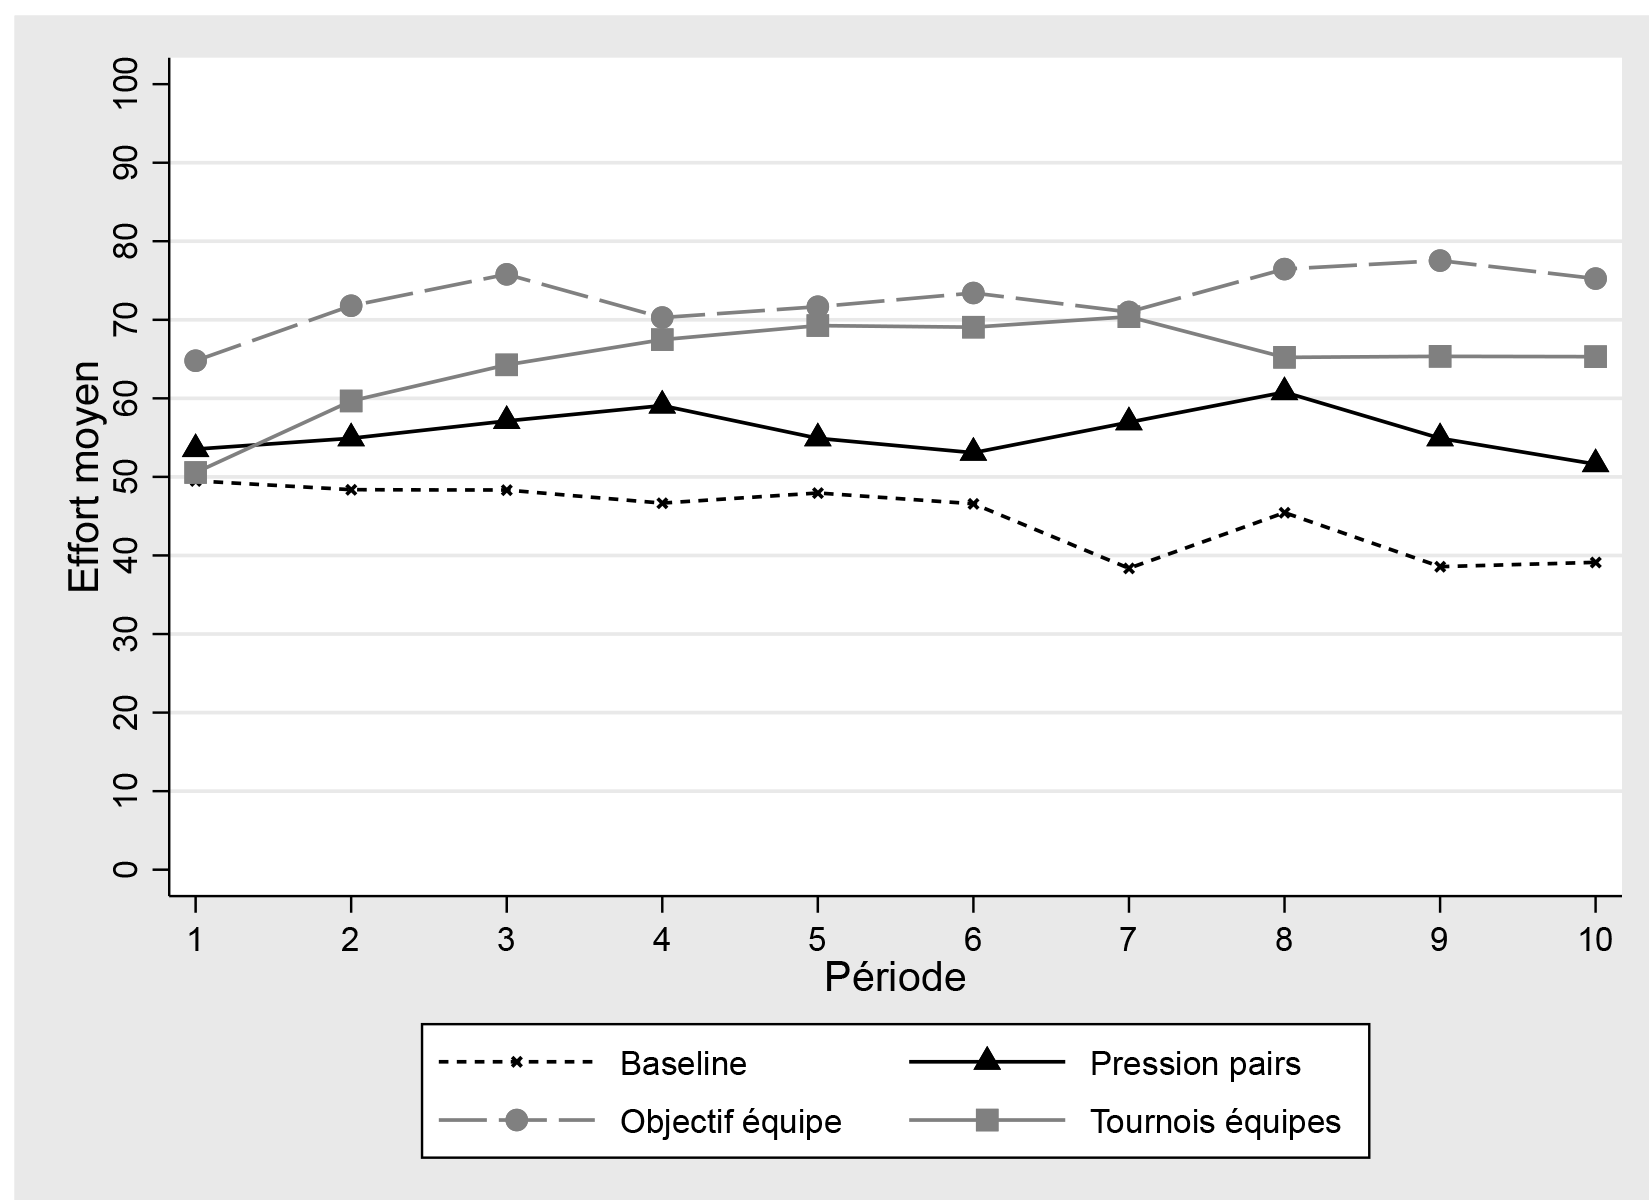
\includegraphics[height=6cm]{05_graph1.png}
\end{figure}

La figure~1 indique que l'effort moyen dans le traitement Baseline
diminue lentement au cours du temps mais reste clairement supérieur à
l'équilibre de Nash de 18,75. Ce résultat est cohérent avec les
résultats obtenus par \textcite{NalbantianSchotter1997} ainsi qu'avec
les résultats issus de la littérature sur les expériences de jeux de
contribution volontaire au financement des biens publics qui ont mis en
évidence deux régularités empiriques fortes~: 1)~les individus
contribuent en moyenne davantage que la prédiction théorique standard et
2)~le niveau moyen de contribution diminue au cours du temps lorsque le
jeu est répété à horizon fini (voir par exemple \textcite{FehrGächter2000}, \textcite{MascletNoussairTuckerVilleval2003}, \textcite{Zelmer2003}, \textcite{SeftonShuppWalker2007} et \textcite{HerrmannThoniGächter2008})\footnote{Des études ont tenté de comprendre ces résultats.
  L'explication la plus plausible repose sur la coopération
  conditionnelle, c'est-à-dire le fait que les individus seraient
  disposés à coopérer mais que cette coopération est conditionnelle à
  l'effort observé chez les autres membres du groupe, ou en fonction de
  leurs croyances concernant les décisions des autres (voir par exemple
  \textcite{KeserVanWinder2000}, \textcite{FischbacherGächter2010} et
  \textcite{ThoniVolk2018}). \textcite{FiguièresMascletWillinger2013}
  proposent une explication alternative basée sur un idéal moral kantien
  faible dans la mesure où celui-ci peut être réévalué en fonction du
  comportement passé des autres.}. La figure~1 indique aussi que le
niveau d'effort paraît plus élevé dans le traitement Pression des pairs
que dans le traitement Baseline. Enfin, l'effort se rapproche de la
solution Pareto dans les systèmes d'incitation centralisés.

Le tableau~2 fournit des statistiques descriptives concernant l'effort
moyen par traitement. Il montre que l'effort moyen dans le traitement
Objectif d'équipe (72,80) est proche de l'optimum de Pareto de 75, et
est significativement plus élevé que dans le traitement Baseline
(44,90). Un test de Mann-Whitney bilatéral sur les efforts moyens par
équipe indique que le niveau d'effort moyen dans le traitement Objectif
d'équipe est significativement plus élevé que dans le traitement
Baseline (MW bilatéral~; \emph{p}~=~0,0065). Le niveau d'effort moyen
dans le traitement Tournois entre équipes (64,66) est aussi
significativement plus élevé que dans le traitement Baseline (MW
bilatéral~; \emph{p}~=~0,016). L'effort moyen est aussi plus élevé dans
le traitement Pression des pairs (55,70) que dans le traitement
Baseline. Toutefois cette différence n'est pas statistiquement
significative (MW bilatéral~; \emph{p}~=~0,1093).

\begin{table}[h]
    \centering
    \caption{Statistiques descriptives par traitement}
\begin{tabular}{m{3.4cm}D{1cm}D{1.5cm}D{1.5cm}D{1.5cm}}
\toprule
                            & Baseline                  & Pression des pairs        & Objectif d’équipe          & Tournois entre équipes\tabularnewline
\midrule
Effort moyen                & 44,90  \varstats{24,17}   & 55,70  \varstats{23,98}   & 72,80  \varstats{22,97}    & 64,66  \varstats{26,20}\tabularnewline
Gain moyen des travailleurs & 54,29  \varstats{22,35}   & 50,11  \varstats{21,41}   & 35,58  \varstats{31,37}    & 64,18  \varstats{47,82}\tabularnewline
Profit moyen des firmes     & 474,57  \varstats{130,54} & 577,51  \varstats{110,42} & 990,88  \varstats{153,73}  & 646,78  \varstats{175,67}\tabularnewline
Richesse globale            & 908,92  \varstats{205,06} & 978,38  \varstats{163,76} & 1275,49  \varstats{191,92} & 1160,18  \varstats{209,93}\tabularnewline
Nombre de participants     & 24                        & 24                        & 24                         & 48\tabularnewline
Observations                & 240                       & 240                       & 240                        & 480\tabularnewline
\bottomrule
\end{tabular}
\notedetableau{Les nombres entre parenthèses sont des écarts types.}
\end{table}

Pour formaliser nos résultats, nous avons réalisé des régressions en
moindres carrés généralisées à effets aléatoires (RE GLS) sur les
déterminants du niveau d'effort. Nous utilisons des effets aléatoires
pour tenir compte de la dimension en panel de nos données et du fait de
l'existence d'effets fixes de traitement. Les résultats de ces
estimations sont présentés dans le tableau~3.

Ce tableau se compose de deux parties. La partie de gauche présente
des estimations sur les déterminants de l'effort. La partie de droite
réplique les estimations de la partie de gauche mais en clustérisant les
écarts types au niveau des équipes afin de contrôler les
interdépendances au sein des équipes. La colonne~1 du tableau indique
que toutes les variables de traitement ont un coefficient positif et
significatif, ce qui suggère qu'introduire un mécanisme d'incitation a
un effet positif sur le niveau d'effort par rapport au traitement de
référence de partage de revenu. La colonne~2 reproduit l'estimation~1
avec l'ajout de variables de tendance (période) et de caractéristiques
démographiques. Les effets de traitement sont robustes à l'introduction
de ces variables. La variable de tendance a un coefficient positif,
indiquant que l'effort moyen augmente au fil du temps\footnote{Notons
  toutefois que cette tendance positive cache des différences entre
  traitements. En effet, des estimations séparées par traitement
  (disponibles sur demande) révèlent une tendance positive pour les
  traitements centralisés et décentralisés, mais une tendance négative
  pour le traitement Baseline.}. La plupart des variables démographiques
sont non significatives à l'exception de la variable «Science
économiques» dont le coefficient est négatif et significatif à
10~\%\footnote{Ce résultat est cohérent avec des études antérieures
  qui ont montré que les étudiants en économie sont en moyenne plus
  enclins à adopter un comportement de passager clandestin dans les
  expériences de biens publics (\textcite{MarwellAmes1981}), et plus
  susceptibles de faire défection dans les jeux du dilemme du prisonnier
  (\textcite{FrankGilovichRegan1993}) et dans les jeux de solidarité
  (\textcite{SeltenOckenfels1998}) ou d'offrir des montants inférieurs
  dans des jeux d'ultimatum (\textcite{CarterIrons1991}). Une hypothèse
  avancée dans la littérature serait l'autosélection, suggérant que les
  individus ayant des tendances intrinsèquement égoïstes seraient plus
  susceptibles de choisir l'économie comme spécialité. Une autre
  explication alternative avance que l'enseignement de l'économie
  encouragerait les étudiants à adopter un comportement plus rationnel
  et maximisateur à l'instar de l'\emph{homo economicus} décrit dans les
  manuels de microéconomie (voir \textcite{BaumanRose2009} pour une
  discussion à ce propos).}.

\begin{table}
    \caption{Déterminants du niveau d’effort}
    \tabcolsep=2pt
    \begin{tabular}{@{}>{\raggedright}p{2cm}>{\raggedleft}p{1cm}l>{\raggedleft}p{1cm}l>{\raggedleft}p{1cm}l>{\raggedleft}p{1cm}l>{\raggedleft}p{1cm}l>{\raggedleft}p{1cm}l @{}}
    \hline
    & Tous &  & Tous &  & Tous sauf traitement & & Tous &  & Tous &  & Tous sauf traitement baseline \tabularnewline
    & & & & & & & \multicolumn{6}{c}{Avec les écarts types clusterisés} \tabularnewline
    \hline
    Var. dép.~: Niveau effort & RE GLS (1) & & RE GLS (2) & & RE GLS (3) & & & & & & & \\
    \hline
    Baseline & Réf. & & Réf. & & & & & & & & & \\
    Pression des pairs & 10,80
    \varstats{4,53} & ** & 11,01
    \varstats{4,58} & ** & Réf. & & 10,80
    \varstats{6,27} & * & 11,01
    \varstats{6,09} & * & Réf. & \\
    Objectif d'équipe & 27,90
    \varstats{4,53} & *** & 27,88
    \varstats{4,65} & *** & 16,69
    \varstats{4,73} & *** & 27,90
    \varstats{4,97} & *** & 27,88
    \varstats{4,70} & *** & 16,69
    \varstats{6,27} & *** \\
    Tournois entre équipes & 19,76
    \varstats{3,92} & *** & 19,73
    \varstats{4,11} & *** & 8,53
    \varstats{4,17} & ** & 19,76
    \varstats{4,75} & *** & 19,73
    \varstats{4,74} & *** & 8,53
    \varstats{6,25} & \\
    Période & & & 0,61
    \varstats{0,24} & ** & 1,06
    \varstats{0,26} & *** & & & 0,61
    \varstats{0,49} & & 1,06
    \varstats{0,56} & * \\
    Homme & & & --~0,17
    \varstats{3,03} & & --~0,43
    \varstats{3,49} & & & & --~0,17
    \varstats{2,35} & & --~0,43
    \varstats{2,86} & \\
    Participation antérieure & & & 3,47
    \varstats{3,69} & & 3,86
    \varstats{3,92} & & & & 3,47
    \varstats{3,57} & & 3,86
    \varstats{3,86} & \\
    Âge & & & 0,36
    \varstats{0,60} & & 0,19
    \varstats{0,77} & & & & 0,36
    \varstats{0,58} & & 0,19
    \varstats{0,88} & \\
    Sciences économiques & & & --~6,53
    \varstats{3,94} & * & --~5,93
    \varstats{4,32} & & & & --~6,53*
    \varstats{3,42} & & --~5,93
    \varstats{3,81} & \\
    Dummy Dernière période & & & --~4,39
    \varstats{2,29} & * & --~5,39
    \varstats{2,53} & ** & & & --~4,39
    \varstats{3,24} & & --~5,39
    \varstats{4,00} & \\
    Constante & 44,90
    \varstats{3,20} & *** & 35,13
    \varstats{12,71} & *** & 47,21
    \varstats{16,79} & *** & 44,90
    \varstats{3,62} & *** & 35,13
    \varstats{13,55} & ** & 47,21
    \varstats{20,91} & ** \\
    \hline
    Observations & 1200 & & 1200 & & 960 & & 1200 & & 1200 & & 960 & \\
    R-squared overall & 0,1292 & & 0,1475 & & 0,08 & & 0,1292 & & 0,1475 & &
    0,08 & \\
    Wald χ\textsuperscript{2} & 44,06 & & 56,58 & & 33,54 & & 34,28 & &
    126,18 & & 100,31 & \\ 
    \hline
    \end{tabular}
    \notedetableau{Les nombres entre parenthèses sont les écarts types. *** \emph{p}~<~0,01, ** \emph{p}~<~0,05, * \emph{p}~<~0,1.}
\end{table}

\newpage

Nous observons aussi un effet de fin de jeu, comme le montre le coefficient négatif et significatif associé à la variable dichotomique «Dernière période». La colonne~3 reproduit
l'estimation présentée dans la colonne~2 mais sur l'échantillon
restreint sans le traitement Baseline. La variable omise est alors la
variable Pression des pairs. Les variables Objectif d'équipe et Tournois
entre équipes ont un coefficient positif et significatif, montrant que
les mécanismes centralisés sont plus efficaces que le mécanisme de
Pression des pairs pour accroître le niveau d'effort. Les estimations
présentées dans la partie droite du tableau donnent des résultats
qualitativement très similaires à ceux présentés dans la partie gauche.
Une exception notable est que la variable Tournois entre équipes n'est
désormais plus significative dans l'estimation~6 après avoir clustérisé
les écarts types. Au total, nos conclusions sont présentées ci-dessous
dans le résultat~1.

% Résultat~1

\vspace{.2cm}
\begin{resultat}
a)~En l'absence de mécanisme d'incitation, le
partage des revenus induit un niveau d'effort faible mais supérieur à
celui théoriquement prévu. b)~La pression des pairs et les deux
mécanismes centralisés conduisent à des niveaux d'efforts des
travailleurs plus élevés que le traitement Baseline de partage des
revenus. c)~Les mécanismes centralisés et en particulier le mécanisme
d'objectif d'équipe génèrent des niveaux d'effort significativement plus
élevés que le mécanisme de pression des pairs.
\end{resultat}


\subsection{Analyse des sanctions dans le traitement Pression des pairs}

Dans cette sous-section, nous analysons les sanctions dans le traitement
Pression des pairs. La figure~2 montre l'évolution du nombre moyen de
points reçus au fil des périodes. Cette figure indique que le nombre de
points reçus diminue régulièrement avec le temps. Ce résultat est
cohérent avec les résultats antérieurs concernant les expériences de
biens publics avec sanction (par exemple \textcite{Nikiforakis2008}~;
\textcite{GächterRennerSefton2008}~; \textcite{MascletVilleval2008}~;
\textcite{NikiforakisEngelmann2011}~; \textcite{DickinsonMasclet2015}).
La raison souvent évoquée dans cette littérature pour expliquer cette
tendance négative est qu'après plusieurs périodes, une fois la
coopération établie au sein de l'équipe, la punition devient crédible et
n'est alors plus nécessaire pour maintenir la coopération (voir \textcite{GächterRennerSefton2008}). Cette baisse tendancielle semble davantage
résulter de la diminution du nombre de points attribués que de celle du
nombre de punisseurs, dont la proportion reste plutôt stable dans le
temps (voir figure~A1 dans l'annexe~\ref{Annexe:Éléments stats}). Il est intéressant de noter que la figure~2 montre qu'il reste un niveau de sanction substantiel
lors de la dernière période, ce qui suggère l'existence de motifs non
stratégiques pour sanctionner\footnote{Ainsi, parmi les
  24~participants du traitement Pression des pairs, 10 punissent au
  cours de la dernière période. Nous les appelons les punisseurs
  ultimes. Une description détaillée de ces punisseurs ultimes est
  présentée à l'annexe~\ref{Annexe:Éléments stats}. Nous remercions un relecteur anonyme pour
  cette suggestion utile.}.

\begin{figure}[h]
    \centering
    \caption{Évolution du nombre moyen de points reçus par travailleur}
    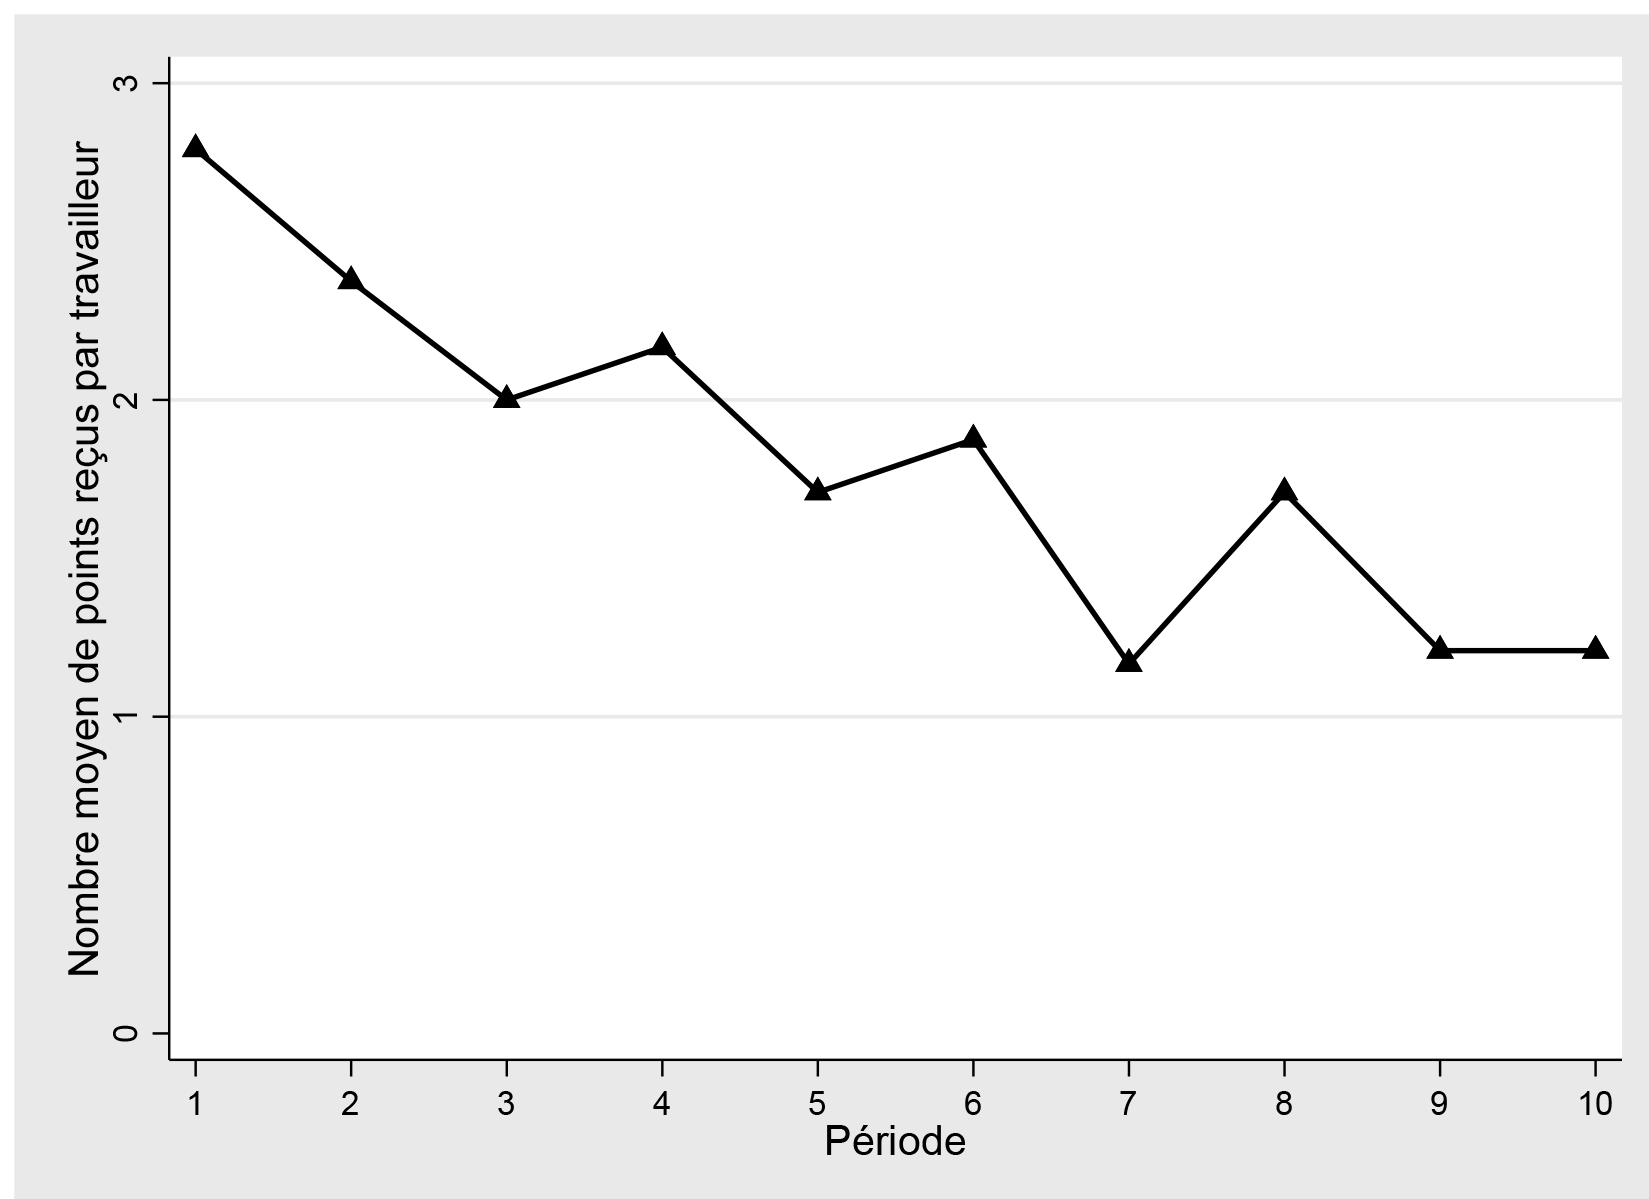
\includegraphics[height=6cm]{05_graph2.png}
\end{figure}

La figure~3 montre le nombre de points de sanction reçus par un
joueur~\emph{i} en fonction de l'écart entre l'effort du joueur~\emph{i}
et l'effort moyen des autres membres de son équipe. La figure~3
indique que davantage de points de sanction sont attribués pour des
écarts négatifs, ce qui est cohérent avec les résultats antérieurs dans
les expériences de bien public avec sanction (\textcite{FehrGächter2000}~; \textcite{MascletNoussairTuckerVilleval2003}; \textcite{HerrmannThoniGächter2008}; \textcite{MascletVilleval2008}). Mais plus
surprenant, la figure~3 indique aussi que les écarts positifs sont
également sanctionnés, bien que dans une moindre mesure. Cependant, un
tel phénomène a déjà été rapporté dans des expériences de bien public
(\textcite{FehrGächter2000}; \textcite{MascletNoussairTuckerVilleval2003}; \textcite{HerrmannThoniGächter2008}; \textcite{MascletVilleval2008}).
De telles punitions ont été classées comme «perverses» ou
«antisociales» (voir par exemple \textcite{CinyabugumaPagePutterman2006}, \textcite{HerrmannThoniGächter2008}, \textcite{NikiforakisNoussairWilkening2012}, \textcite{DenantBoemontMascletNoussair2007} et, plus récemment, \textcite{FuPutterman2018})\footnote{Des études
  ont tenté d'étudier les déterminants des punitions antisociales (voir \textcite{GächterHerrmann2009} pour une discussion détaillée).
  Certains auteurs ont mis en lumière le désir de vengeance (aveugle)
  (\textcite{DenantBoemontMascletNoussair2007}~; \textcite{Nikiforakis2008}~; \textcite{HerrmannThoniGächter2008}). D'autres études
  ont montré l'existence d'une pure volonté de nuire aux autres en
  l'absence d'avantages matériels (\emph{pure nastiness}), qui pourrait
  refléter un désir de domination (\textcite{Zizzo2003}). En outre, les
  individus peuvent manifester de l'aversion envers les coopérateurs,
  punir les non-conformistes et pénaliser les manifestations de
  générosité manifeste (\textcite{CarpenterMatthews2012}~; \textcite{Henrich2006}). D'autres études ont mis en lumière les
  différences culturelles à un niveau macro en matière de punitions
  perverses. Par exemple, \textcite{HerrmannThoniGächter2008} ont
  constaté que les sanctions antisociales ont tendance à se produire
  plus fréquemment dans les sociétés caractérisées par de faibles normes
  sociales de coopération, un faible État de droit et des démocraties
  faibles. Les sanctions antisociales semblent également être souvent
  observées dans les sociétés plus traditionnelles structurées autour de
  solides réseaux privés. Il est intéressant de noter que dans la
  littérature en gestion et économie des ressources humaines, un autre
  motif de sanction antisociale est souvent évoqué, à savoir que
  certains membres d'une équipe peuvent vouloir sanctionner les
  collaborateurs qui coopèrent, pour éviter que la firme ne révise à la
  hausse à l'avenir ses exigences telles que l'objectif à atteindre.
  Toutefois, dans le cadre de notre expérience, ce dernier motif peut
  être exclu puisque les participants étaient informés que l'objectif à
  atteindre était identique à chaque période.}.

\begin{figure}[h]
    \centering
    \caption{Points de sanction reçus et déviation à l'effort moyen des
autres}
    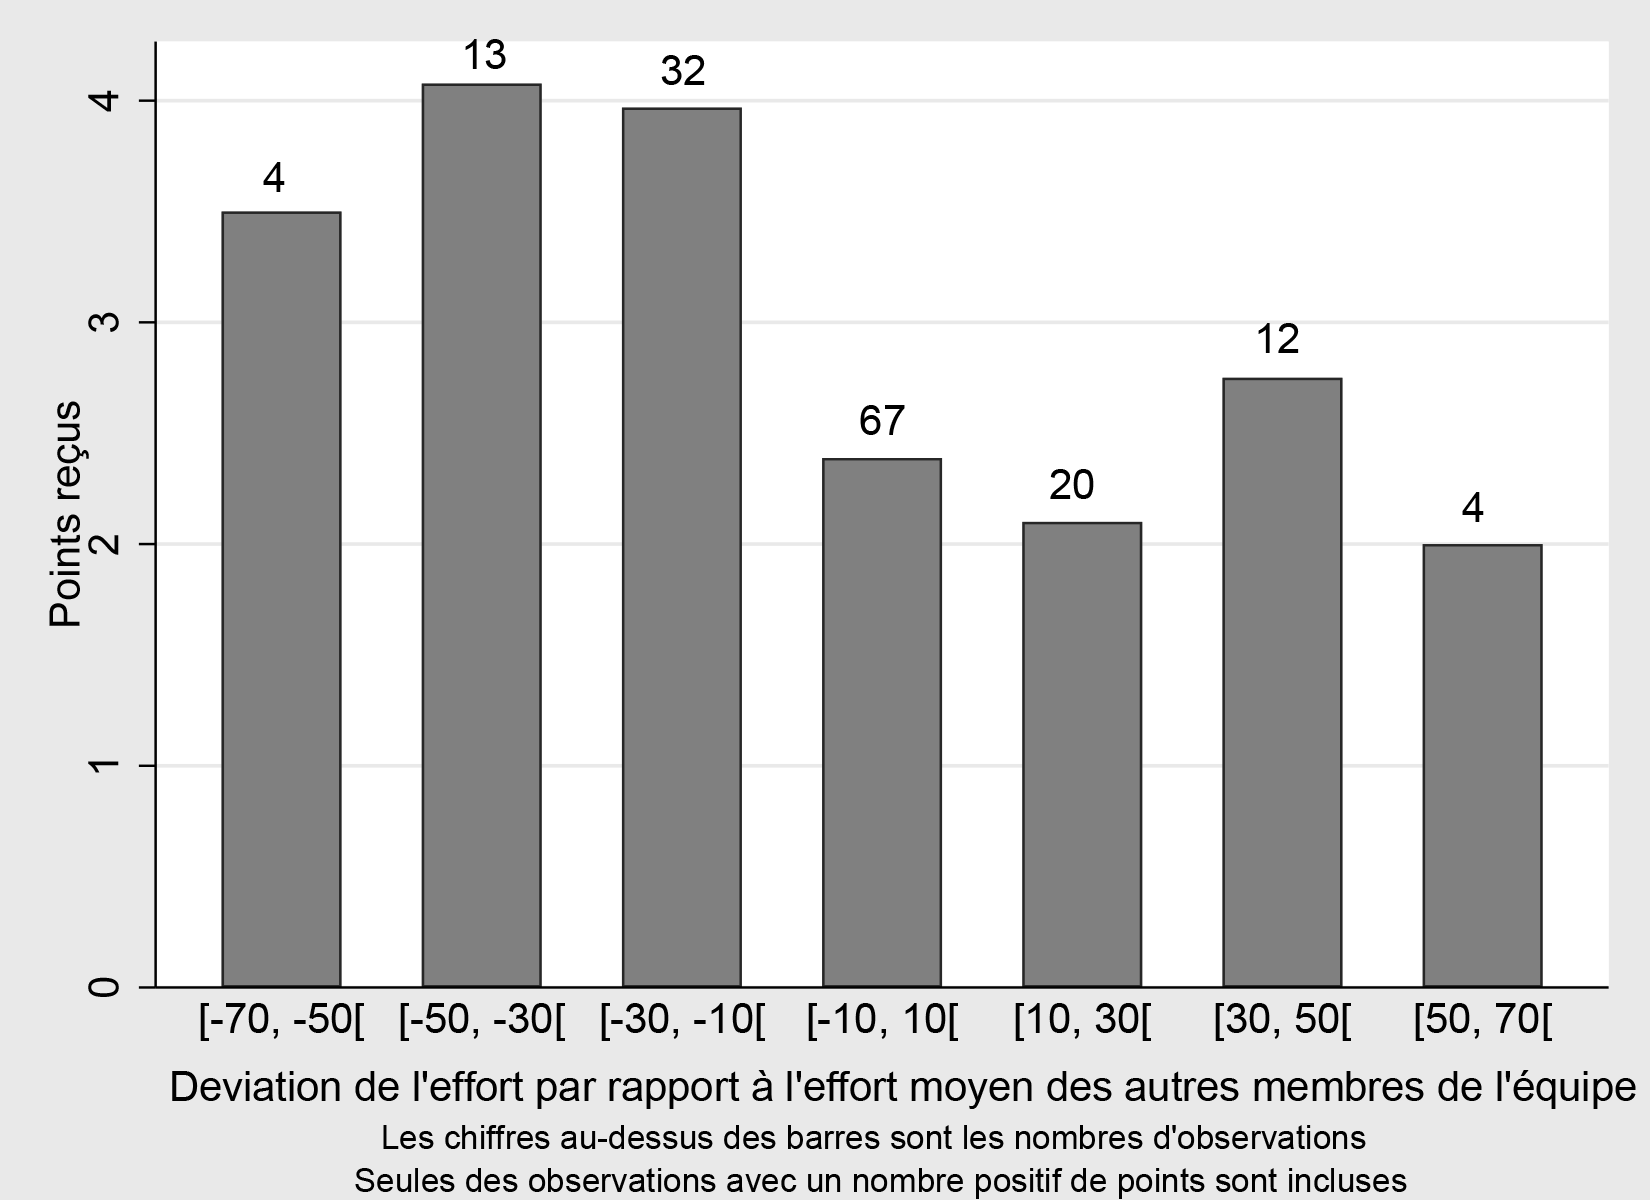
\includegraphics[height=6cm]{05_graph3.png}
\end{figure}

Le tableau~4 présente des estimations sur les déterminants des points de
sanction reçus. La variable dépendante est le nombre de points reçus. On
utilise un modèle Tobit à effet aléatoire afin de contrôler pour les
observations censurées à gauche.

\begin{table}[!ht]
    \renewcommand{\arraystretch}{1.5}
    \caption{Déterminants des points de sanction reçus}\label{tab4}
    \fontsize{8}{10}\selectfont
    \centering
    \begin{tabular}{@{}>{\raggedright}p{7cm}D{2cm}l@{}}
    \toprule
    Var. dép.~: Points de sanction reçus & \multicolumn{2}{>{\centering}p{3.5cm}}{Modèle Tobit effets aléatoires} \tabularnewline
    \midrule
    Effort moyen des autres membres de l'équipe & 0,042 \varstats{0,018} & ** \\
    Valeur absolue de déviation négative par rapport à l'effort moyen des
    autres membres de l'équipe & 0,061 \varstats{0,016} & *** \\
    Déviation positive par rapport à l'effort moyen des autres membres de
    l'équipe & 0,008 \varstats{0,017} & \\
    Période & --~0,25 \varstats{0,07} & *** \\
    Dernière période & 0,20 \varstats{0,70} & \\
    Constante & --~0,77 \varstats{1,21} & \\
    \midrule
    Observations & 240 & \\
    Non censurées & 152 & \\
    LR χ\textsuperscript{2} & 43,69 & \\
    Log Likelihood & --~416,42 &  \\
    \bottomrule
    \end{tabular}
    \notedetableau{Les chiffres entre parenthèses sont des erreurs types.
    ***~\emph{p}~\textless~0,01, **~\emph{p}~\textless~0,05,
    *~\emph{p}~\textless~0,1. La variable «Valeur absolue de déviation
    négative par rapport à l'effort moyen des autres membres de l'équipe»
    est construite comme suit~: elle prend la valeur absolue de l'écart
    négatif de l'effort du travailleur par rapport à l'effort moyen des
    autres membres de son équipe si le travailleur exerce moins d'effort que
    les autres, et zéro sinon. La variable «Déviation positive par rapport
    à l'effort moyen des autres membres de l'équipe» est construite comme
    suit~: elle prend la valeur de l'écart positif de l'effort du
    travailleur par rapport à l'effort moyen des autres au sein de son
    équipe, si le travailleur exerce un effort plus élevé que les autres, et
    zéro autrement.}
    \end{table}

La variable «Valeur absolue de déviation négative par rapport à
l'effort moyen des autres membres de l'équipe» a un coefficient positif
et significatif, indiquant que les travailleurs reçoivent davantage de
sanctions de la part de leurs pairs lorsqu'ils choisissent des efforts
inférieurs à la moyenne de leurs pairs. En revanche, la variable
«Déviation positive par rapport à l'effort moyen des autres membres de
l'équipe» n'est pas significative. La variable «Période» est négative
et significative, indiquant que le nombre de points reçus diminue au fil
du temps. La variable «Dernière période» n'est pas statistiquement
significative, ce qui montre l'absence d'effet de fin de partie. Nos
conclusions sur les comportements de sanction sont résumées dans le
résultat~2.

% Résultat~2.
\vspace{.2cm}
\begin{resultat}
a)~La plupart des points de sanction sont attribués
aux travailleurs fournissant un effort inférieur à la moyenne de leur
équipe. b)~Les sanctions diminuent avec le temps. 
\end{resultat}

\newpage

\subsection{Les gains des travailleurs}

La figure~4 présente l'évolution des gains moyens des travailleurs
par traitement.

\begin{figure}[h]
    \centering
    \caption{Évolution des gains moyens des travailleurs}
    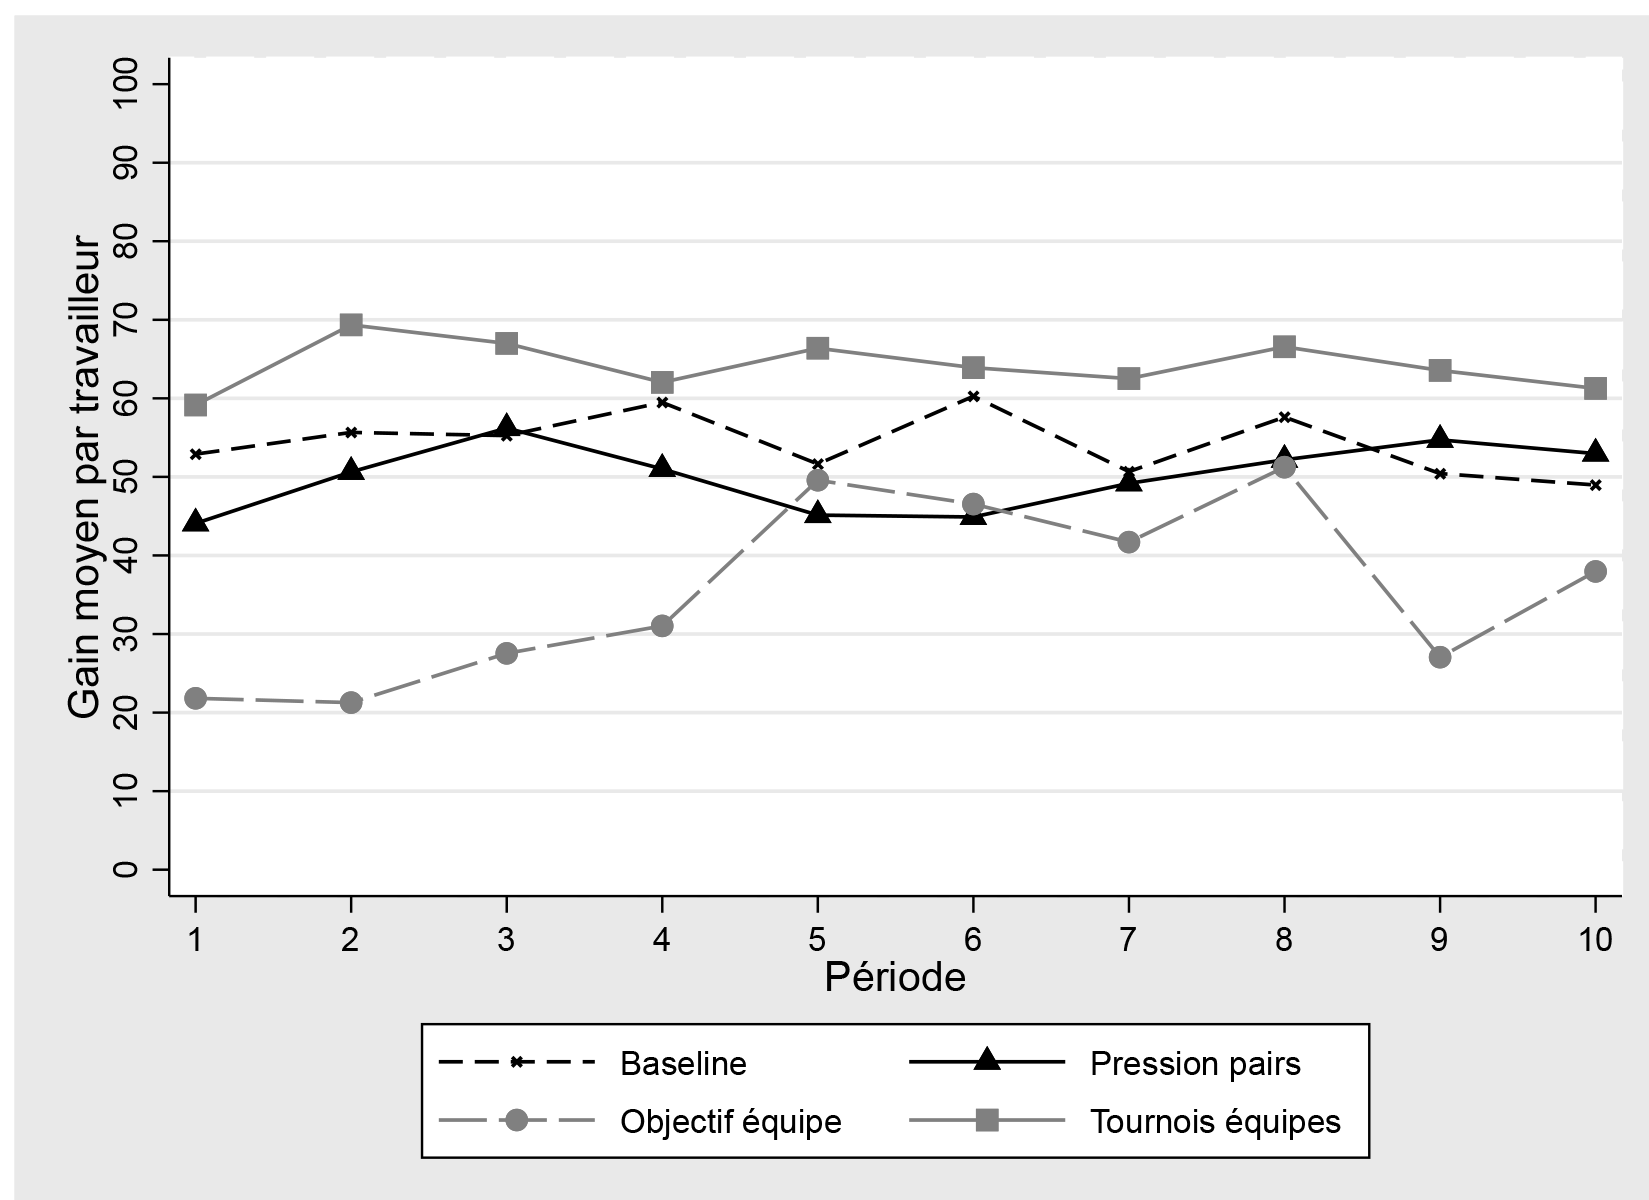
\includegraphics[height=6cm]{05_graph4.png}
\end{figure}

La figure~4 indique que le traitement Objectif d'équipe génère les
gains moyens des travailleurs les plus bas pour presque toutes les
périodes. À l'opposé, les gains sont les plus élevés dans le traitement
Tournois entre équipes. Ces résultats sont confirmés par le tableau~2.
Un test bilatéral de Mann-Whitney indique que les gains des travailleurs
sont significativement inférieurs avec le traitement Objectif d'équipe
qu'avec le traitement Baseline (\emph{p}~=~0,0065). Les gains des
travailleurs sont légèrement plus élevés dans le traitement Tournois
entre équipes que dans le traitement Baseline (\emph{p}~=~0,0547).
Enfin, selon le même test de Mann-Whitney, nous ne pouvons pas rejeter
l'hypothèse nulle selon laquelle les niveaux de gains sont les mêmes
dans le traitement Pression des pairs et dans le traitement Baseline
(\emph{p}~=~0,42). Notons que le tableau~2 fait aussi apparaître des
différences dans les écarts types de gains entre les traitements. En
particulier, l'écart type des gains des travailleurs est plus élevé dans
les systèmes d'incitation centralisés, notamment celui avec Tournois
entre équipes, comparé au traitement Baseline et à la Pression des
pairs. Cela peut s'expliquer par le dispositif de Tournois entre équipes
lui-même, qui impose des transferts entre équipes perdantes et gagnantes
à chaque période, à l'origine d'inégalités considérables de gains.

Le tableau~5 présente les résultats d'estimations sur les déterminants
des gains des travailleurs, des profits des firmes et de la richesse
totale (la somme des profits de la firme et des gains des travailleurs).

\begin{table}
    \caption{Déterminants des gains des travailleurs, des profits des firmes et de la richesse totale (RE GLS)}
\begin{tabular}{@{}L{2.4cm}D{1.8cm}L{0.5cm}D{1.5cm}L{0.5cm}D{1.5cm}L{0.5cm}@{}}
\hline
Var. dép. :              & \multicolumn{2}{>{\centering}m{1.8cm}}{Gains des travailleurs

    (1)}                 & \multicolumn{2}{>{\centering}m{1.5cm}}{Profits des firmes

    (2)}                 & \multicolumn{2}{>{\centering}m{1.5cm}}{Richesse totale

    (3)}\\\midrule
Baseline                 & Réf.                                                  & ~   & Réf.                      & ~   & Réf.                      & ~\\
Pression des pairs       & – 5,88  \varstats{4,34}                               & ~   & 102,94  \varstats{68,82}  & ~   & 69,46  \varstats{99,90}   & ~\\
Objectif d’équipe        & – 22,21  \varstats{5,64}                              & *** & 516,31  \varstats{70,04}  & *** & 366,58  \varstats{110,99} & ***\\
Tournois entre équipes   & 6,11  \varstats{4,45}                                 & ~   & 172,21  \varstats{70,55}  & **  & 251,27  \varstats{99,65}  & **\\
Période – Tendance       & 0,58  \varstats{0,46}                                 & ~   & 4,21  \varstats{6,77}     & ~   & 8,84  \varstats{7,98}     & ~\\
Homme                    & – 5,44  \varstats{3,52}                               & ~   & ~                         & ~   & ~                         & ~\\
Participation antérieure & 9,78  \varstats{6,14}                                 & ~   & ~                         & ~   & ~                         & ~\\
Âge                      & – 0,019  \varstats{0,50}                              & ~   & ~                         & ~   & ~                         & ~\\
Sciences économiques     & 4,73  \varstats{6,41}                                 & ~   & ~                         & ~   & ~                         & ~\\
Dummy Dernière période   & – 4,20  \varstats{4,59}                               & ~   & – 58,34  \varstats{51,31} & ~   & – 91,92  \varstats{65,16} & ~\\
Constante                & 53,61  \varstats{11,61}                               & *** & 457,25  \varstats{65,43}  & *** & 869,49  \varstats{96,55}  & ***\\\midrule
Observations             & 1200                                                  & ~   & 150                       & ~   & 150                       & ~\\
R-squared Overall        & 0,0951                                                & ~   & 0,5786                    & ~   & 0,3331                    & ~\\
Wald $\chi $2            & 339,94                                                & ~   & 74,98                     & ~   & 21,31                     & ~\\\bottomrule
\end{tabular}

\notedetableau{Les chiffres entre parenthèses sont des erreurs types. *** \emph{p}~<~0,01, ** \emph{p}~<~0,05, * \emph{p}~<~0,1. Les erreurs
standards sont clusterisées au niveau du groupe.}
\end{table}

La colonne~1 du tableau~5 indique que la pression des pairs n'augmente
pas significativement les gains des travailleurs. Cela peut résulter des
coûts associés aux sanctions, préjudiciables aux gains des travailleurs
et qui peuvent annuler les bénéfices d'une plus grande coopération. La
variable Tournois entre équipes est également non significative. Une
raison possible est que si ce mécanisme incite les travailleurs à
surperformer, il n'y a cependant finalement qu'une seule équipe
gagnante. Enfin, la variable Objectif d'équipe a un coefficient négatif
et significatif, indiquant que les gains des travailleurs dans ce
traitement sont significativement inférieurs à ceux obtenus dans le
traitement Baseline. Une explication possible est que plusieurs équipes
échouent à atteindre l'objectif, ce qui conduit dans ce cas à des gains
faibles. La figure~5 confirme cette intuition. Elle montre que la
proportion des équipes atteignant l'objectif dans ce traitement est
assez faible, en particulier pendant les premières périodes de jeu.
Cependant, la figure~5 indique également une évolution faible mais
positive de la proportion d'équipes qui atteignent l'objectif au cours
du temps, ce qui suggère l'absence de résignation de la part des
travailleurs. Ce constat est détaillé dans l'annexe~\ref{Annexe:Éléments stats}, dans la sous-section~\ref{Annexe:Évolution dispersion des efforts} qui étudie l'évolution de la dispersion des efforts dans le traitement Objectif d'équipe, pour les équipes qui
atteignent l'objectif, comme pour les équipes qui échouent à l'atteindre.

\begin{figure}[h]
    \centering
    \caption{Proportion d'équipes atteignant l'objectif dans le
traitement Objectif d'équipes}
    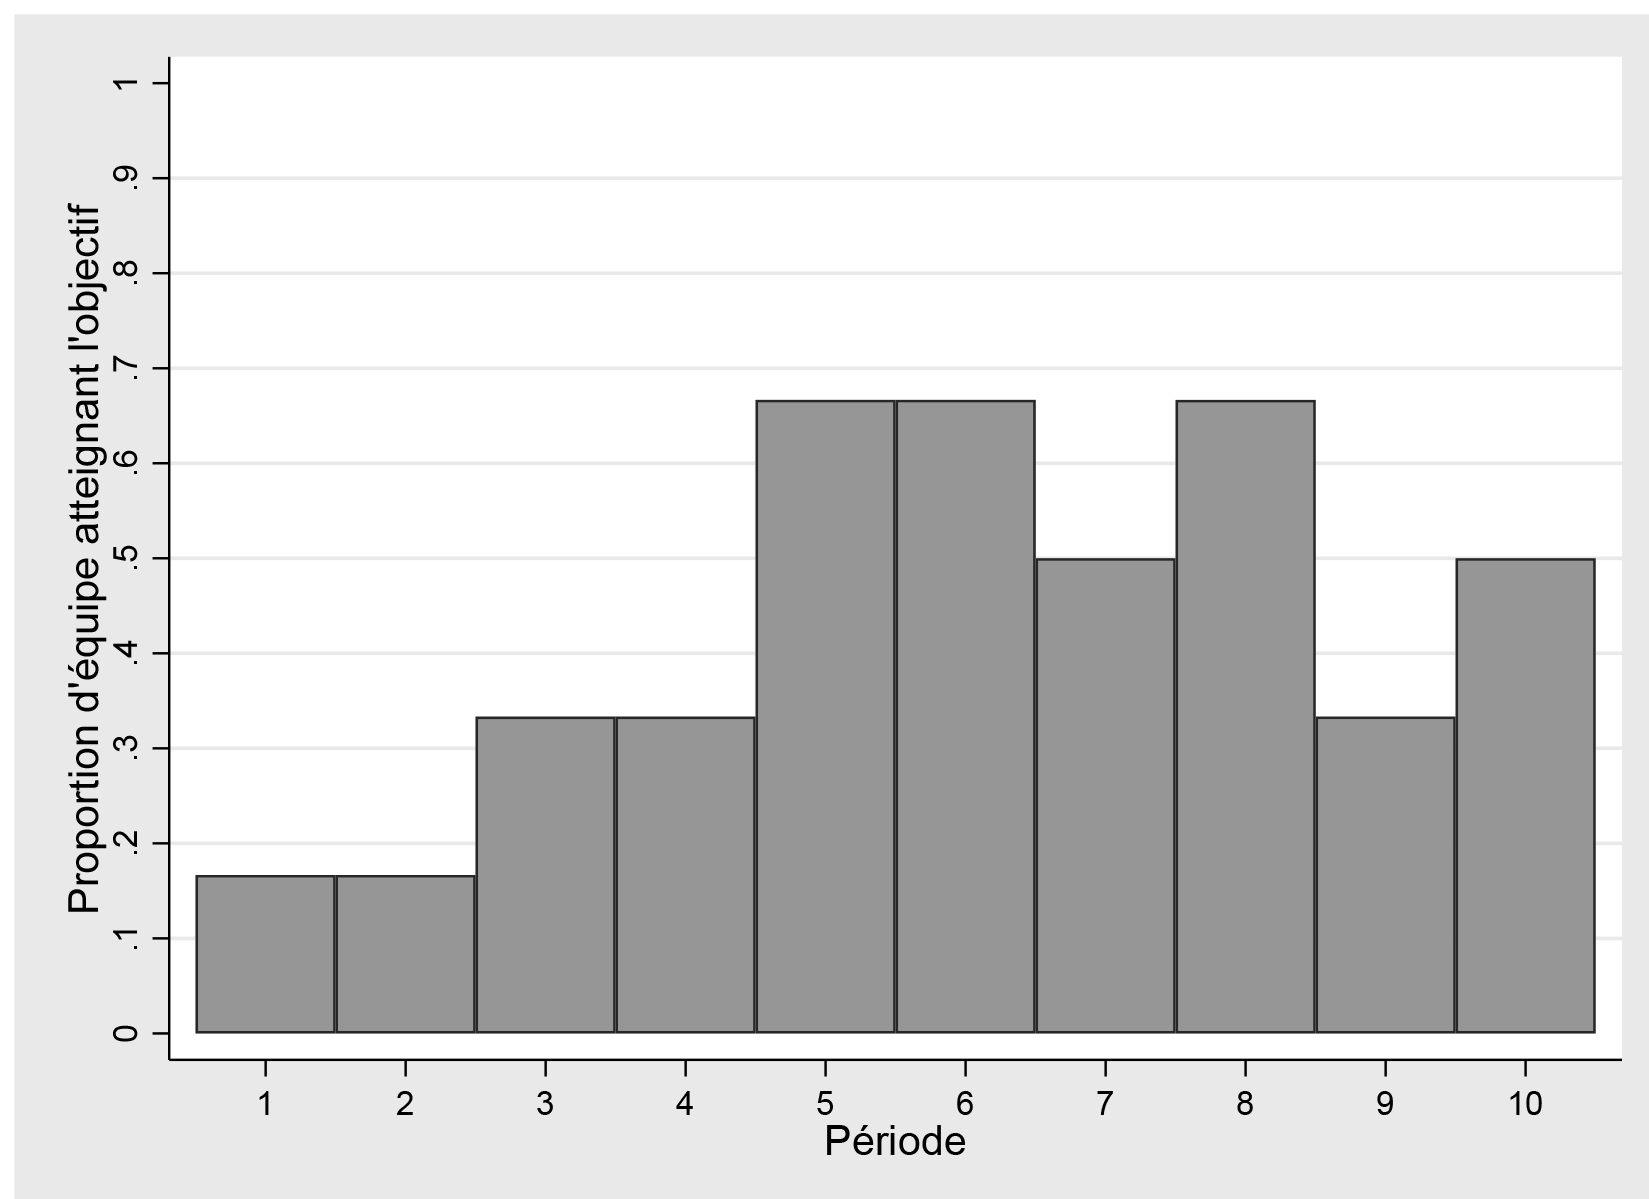
\includegraphics[height=6cm]{05_graph5.png}
\end{figure}

Au total, nos conclusions concernant les gains des travailleurs sont
résumées dans le résultat~3.

\newpage

% Résultat~3
\vspace{.2cm}
\begin{resultat}
a)~La pression des pairs n'améliore pas
significativement les gains moyens des travailleurs par rapport au
traitement Baseline, en raison du coût social des sanctions qui annule
l'effet positif de la pression par les pairs se traduisant par une
coopération accrue. b)~Le mécanisme de tournois entre équipes n'accroît
pas significativement les gains des travailleurs, par rapport au
traitement Baseline, mais augmente considérablement leur dispersion.
c)~Dans le traitement Objectif d'équipe, les gains des travailleurs sont
beaucoup plus faibles et plus dispersés que dans le traitement Baseline,
car de nombreuses équipes échouent à atteindre l'objectif.
\end{resultat}


\subsection{Les profits des firmes}

La figure~6 ci-dessous montre l'évolution du profit moyen des firmes,
par traitement. Le tableau~2 et la figure~6 montrent que les profits
des firmes sont les plus élevés dans le traitement Objectif d'équipe et
les plus faibles dans le traitement Baseline.

\begin{figure}[h]
    \centering
    \caption{Évolution du profit moyen des firmes}
    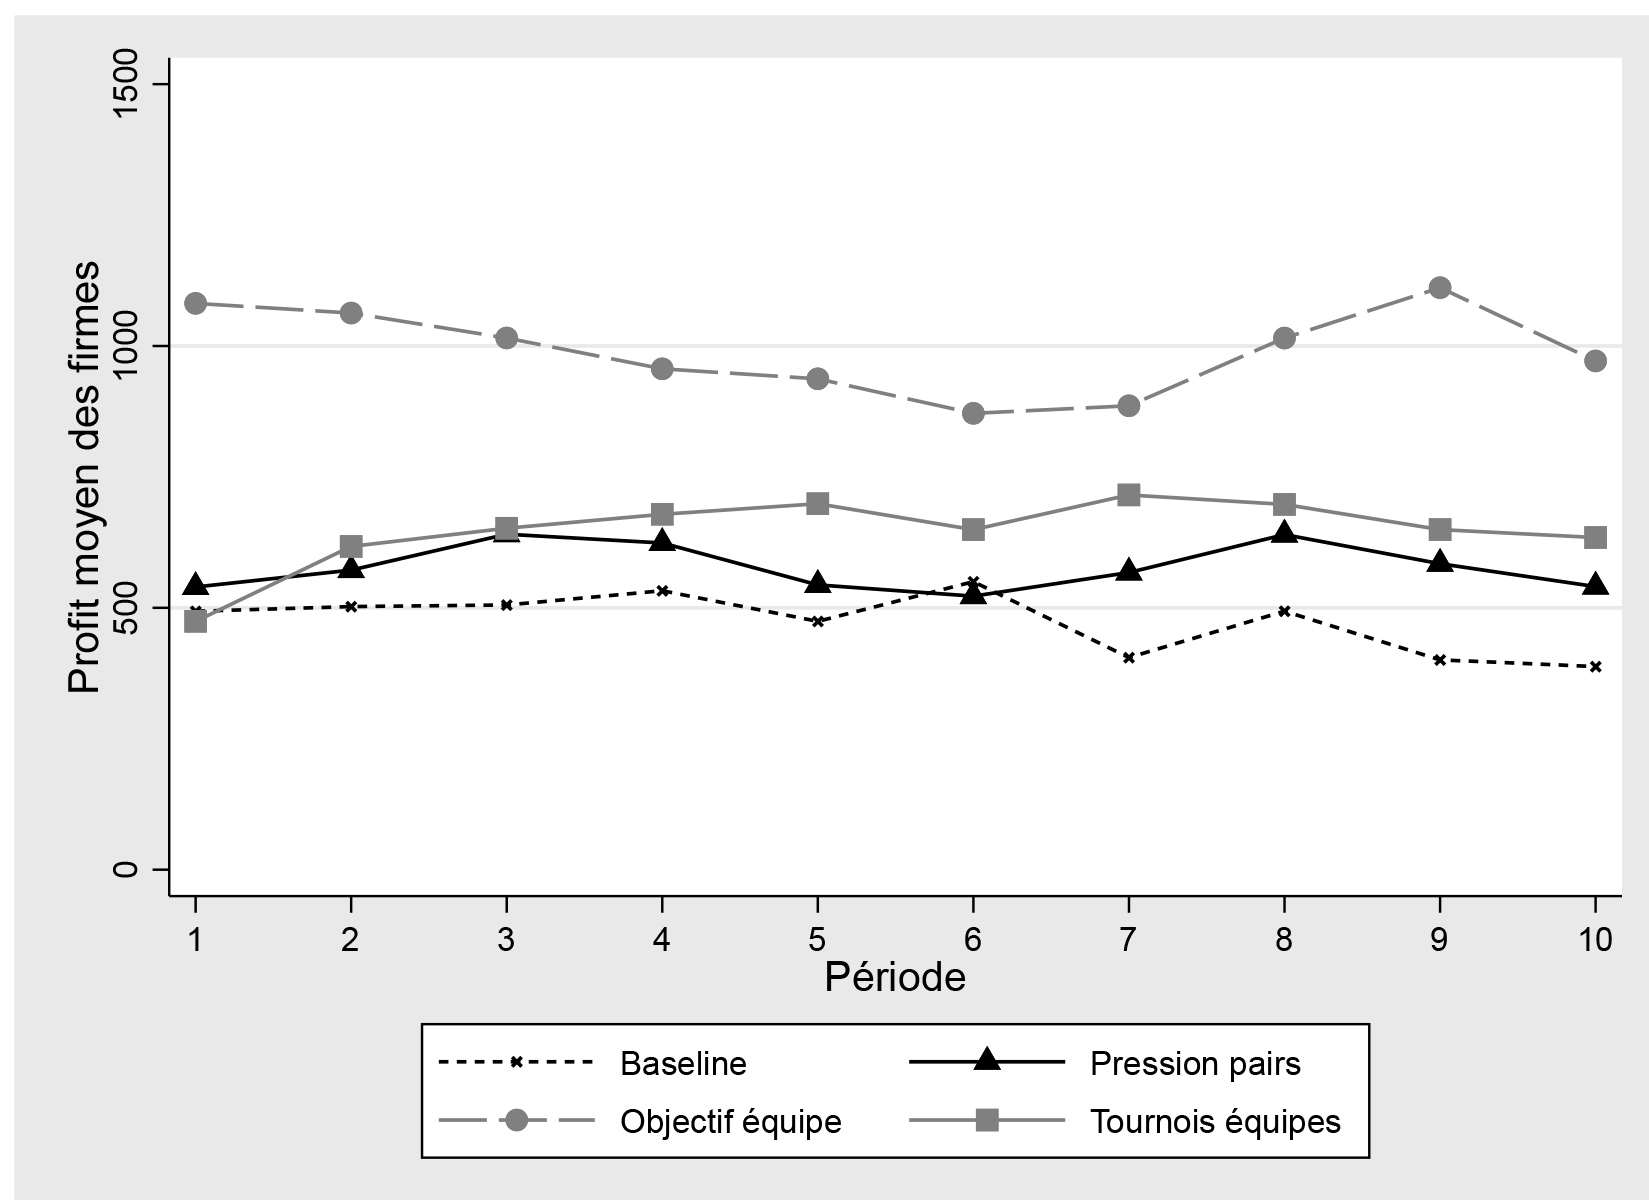
\includegraphics[height=6cm]{05_graph6.png}
\end{figure}

La colonne~2 du tableau~5 présente les résultats d'une estimation des
déterminants du profit des entreprises. Cette estimation indique que les
profits des firmes sont significativement plus élevés dans le traitement
Objectif d'équipe et, dans une moindre mesure, dans le traitement
Tournois entre équipes, comparés au traitement Baseline. La variable
Pression des pairs n'est pas significative, ce qui montre que ce
mécanisme n'améliore pas significativement les profits des firmes. Les
tests effectués sur les coefficients de la colonne~2 du tableau~5,
présentés dans la sous-section~\ref{Annexe:Significativité différences de profits} de l'annexe~\ref{Annexe:Éléments stats}, révèlent que
les profits des firmes sont significativement plus élevés dans le
traitement Objectif d'équipe que dans les traitements Pression des pairs
et Tournois entre équipes, mais qu'il n'y a pas de différence
significative de profits des firmes entre Pression des pairs et Tournois
entre équipes.

Nos conclusions concernant les profits des firmes sont présentées dans
le résultat~4.

% Résultat~4.
\vspace{.2cm}
\begin{resultat}
a)~Introduire un mécanisme centralisé augmente les
profits des firmes par rapport au traitement Baseline. b)~Les profits
des firmes sont les plus élevés avec le traitement Objectif d'équipe.
c)~La pression des pairs n'entraîne pas d'augmentation de profits des
firmes par rapport au traitement Baseline.
\end{resultat}

\subsection{À qui profite principalement l'introduction de mécanismes
(dé)centralisés~: la firme ou les travailleurs~?}

Dans cette section, nous examinons qui bénéficie principalement de
l'introduction de mécanismes (dé)centralisés. À cette fin, nous
considérons la richesse totale comme la somme des profits de la firme et
des gains des travailleurs et étudions comment elle est partagée entre
les deux parties.
Le tableau~2 plus haut montre la richesse par traitement. Il indique que
la richesse est la plus faible dans le traitement Baseline et la plus
élevée dans le traitement Objectif d'équipe, où le profit élevé des
firmes fait plus que compenser les faibles gains des travailleurs.
La colonne~3 du tableau~5 montre que la richesse totale est maximale
avec les mécanismes centralisés. Le mécanisme décentralisé de Pression
des pairs n'a pas d'effet significatif sur la richesse totale comparé au
traitement Baseline. Les tests sur les coefficients de la colonne~3 du
tableau~5, présentés dans la sous-section~\ref{Annexe:Significativité différences de profits} de l'annexe~\ref{Annexe:Éléments stats}, confirment que la richesse totale est significativement plus élevée dans
les traitements Objectif d'équipe et Tournois entre équipes que dans le
traitement Pression des pairs, mais que la différence entre les
traitements Objectif d'équipe et Tournois entre équipes n'est pas
significative.
La figure~7 montre la composition de la richesse totale par
traitement. Il indique que cette composition diffère fortement entre
traitements, soulignant les arbitrages et les aspects politiques
associés au choix d'un traitement (voir les figures~A8-A11 dans
l'annexe~\ref{Annexe:Éléments stats} pour une analyse séparée par traitement sur les évolutions de la composition de la richesse totale au fil des périodes). La
figure~7 montre qu'alors que la richesse totale est partagée presque
à égalité entre la firme et les travailleurs dans le traitement Baseline
et, dans une certaine mesure, dans les traitements Pression des pairs et
Tournois entre équipes, à l'inverse, cette répartition est nettement en
faveur de la firme dans le traitement Objectif d'équipe.

\begin{figure}[h]
    \centering
    \caption{Composition de la richesse totale}
    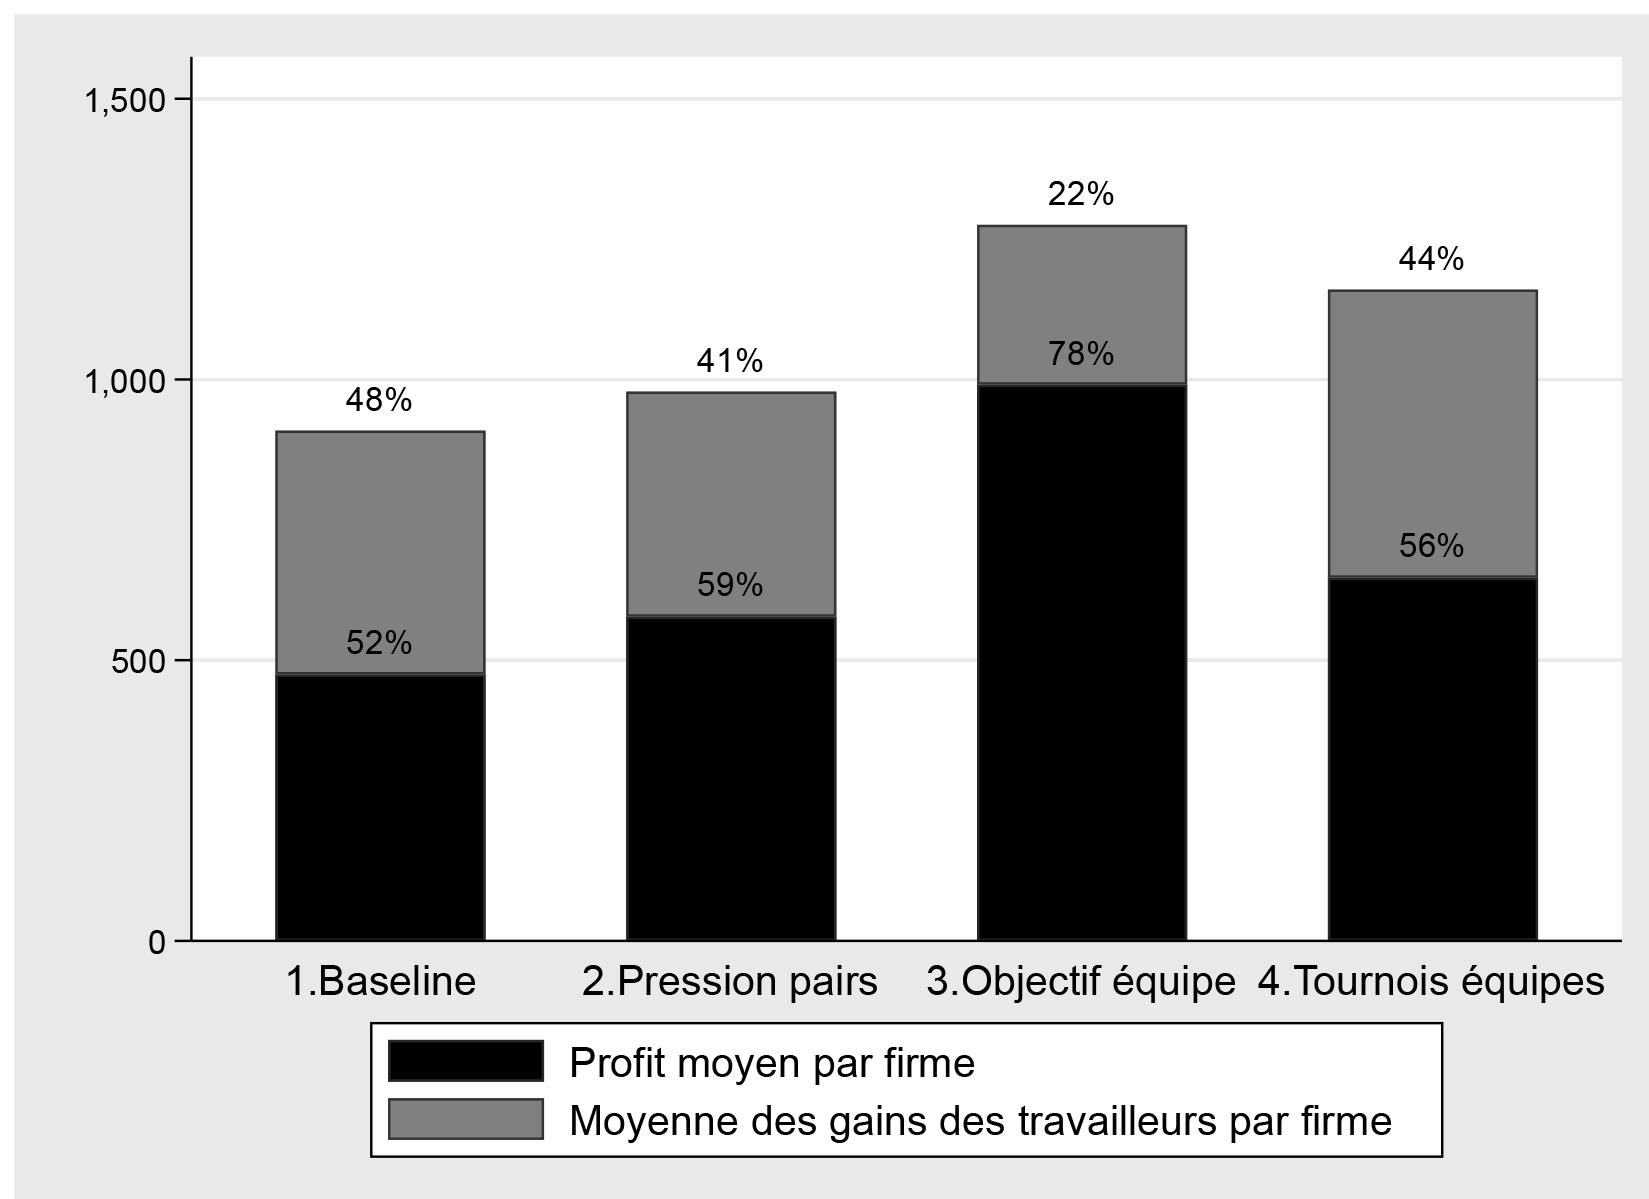
\includegraphics[height=5.5cm]{05_graph7.png}
\end{figure}

Nos principales conclusions concernant la répartition de la richesse
totale entre firme et travailleurs se résument comme suit~:

% Résultat~5.
\vspace{.2cm}
\begin{resultat}
a)~La richesse totale (c'est-à-dire la somme des
profits de la firme et des gains des travailleurs) est plus élevée avec
les mécanismes centralisés qu'avec le traitement Baseline. b)~Dans le
mécanisme avec Objectif d'équipe, les firmes captent la plus grande part
de la richesse totale. c)~La pression des pairs n'augmente pas de
manière significative la richesse totale par rapport au traitement
Baseline.
\end{resultat}


\section{Discussion et conclusion}
\label{section:discussion et conclusion}

Nous avons étudié l'efficacité et l'efficience de différents mécanismes
visant à dissuader les comportements de passager clandestin au sein
d'équipes de travail, en comparant les systèmes centralisés (basés sur
des objectifs et tournois d'équipes) et décentralisés (pression des
pairs).

Nos résultats montrent premièrement qu'en l'absence de mécanismes
d'incitation, l'effort est sujet à un phénomène de passager clandestin,
bien que moins sévère que ne le prédit la théorie.

Deuxièmement, en conformité avec les résultats obtenus précédemment dans
des expériences de contribution volontaire au financement de biens
publics avec sanction, nous observons que la pression des pairs accroît
l'effort par rapport au traitement Baseline. Toutefois, son impact reste
faible et les gains des travailleurs ne sont pas augmentés par rapport
au traitement Baseline. La raison à cela est que les coûts associés aux
sanctions annulent les gains d'une coopération accrue engendrée par la
pression des pairs.

Troisièmement, les mécanismes centralisés sont plus efficaces que la
pression des pairs pour accroître l'effort. En particulier, le mécanisme
d'objectif d'équipe conduit à un niveau d'effort proche du niveau
optimal de Pareto, mais au prix de gains plus faibles et plus inégaux
pour les travailleurs. En effet, de nombreuses équipes échouent souvent
à atteindre l'objectif. À l'opposé, ce système conduit à une forte
augmentation des profits des firmes.

Quatrièmement, la mise en place de tournois entre équipes accroît
significativement les niveaux d'effort, mais sans augmenter
significativement les gains moyens des travailleurs, et cela entraîne de
grandes inégalités de gains entre travailleurs du fait des transferts
entre équipes gagnantes et équipes perdantes.

Cinquièmement, la richesse totale est maximisée avec les mécanismes
centralisés, et en particulier avec le mécanisme d'Objectif d'équipe.
Cependant, avec ce mécanisme, la richesse est très inégalement partagée
entre la firme et les travailleurs, la première en recevant la plus
grande part.

Globalement, ces résultats mettent en lumière le fait qu'il est
important, lorsque l'on envisage la mise en place d'un système de
rémunération, de prendre en compte plusieurs dimensions dont
l'efficacité, l'efficience, mais également la manière dont la richesse
est partagée entre les parties prenantes, au risque sinon de générer des
tensions sources d'inefficiences futures. En effet, si deux mécanismes
peuvent aboutir à des niveaux similaires de richesse, l'un mettant
l'accent sur des profits plus élevés et l'autre donnant la priorité à
des gains substantiels pour les travailleurs, la décision sur le
mécanisme à mettre en œuvre peut nécessiter un arbitrage politique
nuancé\footnote{Nous remercions ici un évaluateur anonyme pour cette
  remarque pertinente.}.

Notre étude a bien sûr des limites et peut susciter certaines
interrogations. Une première interrogation porte sur la validité externe
de nos résultats. Ainsi, dans quelle mesure ceux-ci peuvent-ils
être étendus à d'autres populations et d'autres contextes du monde réel,
au-delà du laboratoire~? On peut en effet raisonnablement douter de la
possibilité d'extrapoler des résultats de laboratoire, qui constitue un
environnement pouvant être perçu comme artificiel et manquant de
réalisme (voir par exemple \textcite{BerkowitzDonnerstein1982} et
\textcite{Colquitt2008}). En outre, on peut se demander si un petit nombre
de participants, étudiants pour la plupart, sont représentatifs de
populations plus larges (\textcite{LevittList2007}, \textcite{LevittList2007-1}).
Répondre à cette question nécessite d'abord de définir la notion de
validité externe. À l'instar de \textcite{KesslerVesterlund2015} et
\textcite{LevittList2007}, il convient de distinguer entre validité
externe quantitative et qualitative. En effet, si nos résultats ne
peuvent prévoir la magnitude des effets considérés (faible validité
externe quantitative), ils peuvent néanmoins avoir une bonne validité
externe qualitative ou directionnelle, c'est-à-dire donner une certaine
indication sur la direction de l'effet considéré\footnote{Cela a été
  joliment résumé par \textcite{LevittList2007}, p.~351, dans les
  termes suivants~: «\emph{It is likely that the qualitative findings
  of the lab are generalizable, even when the quantitative magnitudes
  are not}.» La distinction entre résultats quantitatifs et qualitatifs
  est fortement liée à la question de la validité externe des résultats
  expérimentaux. Les résultats quantitatifs font référence à
  l'«ampleur» ou à la «magnitude» d'un effet tandis que les
  résultats qualitatifs font référence à la «direction» d'un effet.}.
En d'autres termes, la question n'est pas de savoir dans quelles
proportions les mécanismes centralisés surpassent le système
décentralisé mais de savoir quelle est la direction de l'effet. Le
critère d'évaluation de la validité externe doit se concentrer sur la
question de savoir si le signe de l'effet reste cohérent dans différents
environnements. De plus, notre expérience doit être considérée comme une
première étape qui appelle à être reproduite (\textcite{Camerer2015}).
Lorsqu'un effet a été reproduit dans l'environnement contrôlé du
laboratoire, et dans un cadre bien défini, son ampleur peut être alors
évaluée sur le terrain et dans le contexte souhaité. \textcite{Schram2005},
p.~232, discute de ce point en utilisant l'analogie avec les tests d'un
nouvel avion en soufflerie~: «\emph{After a theoretical design, a test}
[of a new airplane] \emph{in a wind tunnel is the stage of
laboratory experimentation. If it does not ``crash'' in this experiment,
the plane is not immediately used for the transport of passengers,
however. One will typically conduct further tests in the wind tunnel
under extreme circumstances. In addition, further testing including
``real'' flights without passengers will be conducted.~}»

Une extension naturelle de notre étude consisterait à tester si des
professionnels présenteraient un comportement similaire à la fois en
laboratoire et dans leur contexte de travail (\textcite{HarrisonList2004} appellent de telles expériences des expériences
artefactuelles de terrain de type «\emph{lab in the field}» ou
«\emph{field in the lab}»). Cela nous permettrait de vérifier si nos
résultats sont valables dans d'autres environnements, et d'accroître
ainsi leur validité externe.

Une autre piste de recherche consisterait à mener des traitements
supplémentaires visant à dissocier les effets de réputation des effets
des mécanismes incitatifs\footnote{Nous remercions un rapporteur
  anonyme pour cette suggestion.}. Par exemple, comparer nos traitements
selon que la composition des équipes reste inchangée au cours du temps
(«\emph{Partner matching}») ou qu'elle change à chaque période
(«\emph{Stranger marching}») permettrait d'identifier d'éventuels
effets réputationnels. Une autre piste d'extension consisterait
également à enrichir notre cadre théorique en considérant le rôle de
l'aversion au risque, des préférences sociales (voir \textcite{FehrSchmidt1999}) ou des intentions (\textcite{Rabin1993}). Enfin, une extension
de nos travaux consisterait à chercher à rendre la pression des pairs
plus efficace. Ainsi sa performance serait-elle améliorée si cette
pression était centralisée entre les mains d'un leader d'équipe~?

{\sloppy % Justification du texte plus "laxiste"
\printbibliography
}

\newpage

\begin{appendices}

%ANNEXES

\section{Prédictions théoriques}
\label{Annexe:Prédictions}

\subsection{Traitement Baseline}
\label{Annexe:Traitement Baseline}

\vspace{0,3cm}
Dans le traitement Baseline, le gain de chaque membre~\emph{i} de
l'équipe~\emph{j},\emph{π\textsubscript{i}}\textsubscript{,\emph{j}},
est donné par~:
\begin{equation}
    \frac{\pi_{i,j} = 1,5\left( \sum_{1}^{4}e_{i,j} + \varepsilon \right)}{4} - \left( \frac{e_{i,j}^{2}}{100} \right) + 10.
\end{equation}

Avec la condition de premier ordre~:
\begin{equation}
  \frac{\partial\pi_{i,j}}{\partial e_{i,j}} = \frac{1,5}{4} - \frac{2e_{i,j}}{100} = 0.
\end{equation}

On déduit facilement des équations~(A1) et (A2) que les gains de
\emph{i} sont maximisés pour l'effort \(e_{ij}^{*} = 18,75\), qui
correspond à l'équilibre de Nash de ce jeu. Cet effort est en dessous du
niveau d'effort Pareto-optimal de 75. Le jeu étant répété un nombre fini
de fois, le seul équilibre parfait en sous-jeux du jeu, consiste pour
tous les joueurs à fournir un effort \(e_{ij}^{*} = 18,75\) à chaque
période.

Les prédictions théoriques précédentes reposent sur l'hypothèse standard
que les individus poursuivent uniquement leur intérêt matériel
personnel, étant dépourvus de préférences sociales. Or plusieurs
résultats empiriques suggèrent que cette hypothèse ne se vérifie pas
toujours. Par exemple, dans un contexte similaire de jeu d'effort avec
partage de revenus, \textcite{NalbantianSchotter1997} observent que le
niveau d'effort se maintient au-dessus du niveau de l'équilibre de Nash
tout en diminuant toutefois au cours du temps. Ces résultats sont
également cohérents avec la littérature sur les expériences de biens
publics qui a documenté deux fortes régularités empiriques~: 1)~le fait
que les individus contribuent plus que ce que prédit le modèle théorique
standard au bien public~; et 2)~que cette contribution moyenne diminue
au cours du temps lorsque le jeu est répété sur un horizon fini (voir \textcite{Ledyard1995}, \textcite{Andreoni1995}, \textcite{Croson1996}, \textcite{KeserVanWinder2000}, \textcite{FehrGächter2000}, \textcite{MascletNoussairTuckerVilleval2003}, \textcite{HerrmannThoniGächter2008}, \textcite{KriegSamek2017}). La littérature propose trois explications majeures à ces
phénomènes~: les effets d'apprentissage (\textcite{Andreoni1988})\footnote{L'hypothèse d'effets d'apprentissage postule que
  les contributions initiales élevées proviennent de la confusion et des
  erreurs des sujets, diminuant progressivement à mesure qu'ils
  identifient la possibilité d'obtenir des gains plus élevés avec des
  contributions réduites. Toutefois l'hypothèse d'effets d'apprentissage
  semble incompatible avec l'«effet de \emph{restart}» (voir \textcite{Andreoni1988}).}, les comportements stratégiques (\textcite{KrepsMilgromRobertsWilson1982})\footnote{L'hypothèse de comportement stratégique, ancrée
  dans l'hypothèse du «\emph{crazy player}» (\textcite{KrepsMilgromRobertsWilson1982}), ou l'absence de connaissance commune de la rationalité,
  postule que si les acteurs rationnels croient qu'il existe un
  \emph{crazy player} dans le groupe, contribuant positivement au cours
  de la période~1, alors il devient rationnel pour eux d'adopter une
  stratégie coopérative au début, en diversifiant les stratégies au fur
  et à mesure de la progression du jeu répété. Cependant, les résultats
  d'\textcite{Andreoni1988} tendent à remettre en question cette hypothèse
  en tant qu'explication plausible de la diminution de la contribution
  moyenne.} et la coopération conditionnelle (\textcite{FischbacherGächterFehr2001}). Alors que les résultats empiriques suggèrent que
l'apprentissage ou les comportements stratégiques ne jouent qu'un rôle
limité dans l'explication de la baisse du niveau de contribution, la
plupart des études ont concentré leur attention sur le rôle joué par la
coopération conditionnelle, c'est-à-dire le fait que les individus
conditionnent leurs comportements sur l'observation du comportement des
autres, ou sur leurs croyances concernant le comportement des autres,
dans des jeux de bien public simultanés et répétés de manière finie (par
exemple \textcite{KeserVanWinder2000}, \textcite{FischbacherGächterFehr2001}, \textcite{Croson2007} et \textcite{FischbacherGächter2010}).
D'autres travaux ont avancé l'hypothèse de coopération conditionnelle
imparfaite (voir \textcite{FischbacherGächter2010}). Enfin d'autres
études (\textcite{FiguièresMascletWillinger2013}~; \textcite{MascletDickinson2019}) proposent des modèles de comportement avec une
motivation morale kantienne faible, avec l'idée que les agents révisent
à la hausse ou à la baisse leur idéal moral selon la contribution des
autres (voir \textcite{BrekkeKverndokkNyborg2003}).

À partir de cette littérature, nous pouvons raisonnablement énoncer la
conjecture suivante~:

\vspace{0,2cm}
H1~: \emph{Les effets combinés d'une motivation morale faible et d'une
réciprocité conditionnelle conduisent à une baisse de l'effort au cours
du temps}.

\subsection{Traitement avec Pression des pairs}

Le traitement avec Pression des pairs est similaire au traitement
Baseline, sauf qu'après le choix de l'effort, une deuxième étape est
ajoutée où chaque membre de l'équipe observe les niveaux d'effort de ses
équipiers et peut utiliser son revenu forfaitaire Ω (fixé à 10 dans
l'expérience) pour leur attribuer des points de sanction. La sanction
est coûteuse à la fois pour le joueur sanctionné et pour celui qui
sanctionne. Plus précisément, si le travailleur~\emph{i} attribue
\emph{p\textsubscript{izj}}~points de sanction au travailleur~\emph{z},
cela réduit les gains du travailleur~\emph{i} de
\emph{p\textsubscript{izj}} et ceux du travailleur~\emph{z} de
3\emph{p\textsubscript{izj}}. Le travailleur~\emph{i} ne peut utiliser
plus que son revenu forfaitaire~Ω pour sanctionner ses trois
coéquipiers. Ainsi~: \(\sum_{z \neq i}^{}p_{izj} \leq \Omega\). Dans le
cadre de l'expérience, les gains ne peuvent être strictement négatifs.
Pour chaque période, le gain final de chaque travailleur est donné par
l'équation~:
\begin{equation}
    \pi_{i,j} = \max\left( 1,5\frac{\left( \sum_{1}^{4}{e_{ij} + \varepsilon} \right)}{4} - \frac{e_{ij}^{2}}{100} + 10 - \sum_{i \neq z}^{}p_{izj} - 3\sum_{z \neq i}^{}p_{zij},0 \right).
\end{equation}

Par induction à rebours, l'équilibre parfait en sous-jeux est
$e_{ij}^{*}=18,75$, $p_{izj}=~0$. En effet, personne n'est incité à
sanctionner en seconde étape dans la mesure où sanctionner est coûteux.
Anticipant cela, les travailleurs minimisent leur effort lors de la
première étape. L'équilibre parfait unique du sous-jeu est donc celui
d'un faible niveau d'effort (\(e_{ij}^{*} = 18,75\)) et aucune sanction
attribuée. Puisque le jeu est un jeu répété à horizon fini, les
prédictions théoriques s'appliquent à l'ensemble des périodes.

Toutefois, à l'instar du traitement Baseline, nous pouvons relâcher
l'hypothèse d'individus autocentrés et considérer les prédictions des
modèles basés sur l'hypothèse de coopération conditionnelle imparfaite
(\textcite{FischbacherGächterFehr2001}~; \textcite{FischbacherGächter2010}) et/ou la faible motivation morale (\textcite{FiguièresMascletWillinger2013}~; \textcite{MascletDickinson2019}). Dans ces
modèles, il existe des situations où les coopérateurs conditionnels
peuvent être incités à punir, ce qui rend la décision de punition
crédible et conduit à un niveau d'effort plus élevé. Sur la base de
cette littérature, nous pouvons donc formuler l'hypothèse suivante H2.

\vspace{0,2cm}
H2~: \emph{Sous certaines conditions et sous l'hypothèse de coopération
conditionnelle et/ou d'une motivation morale faible, les individus
peuvent être incités à sanctionner en seconde étape du jeu, rendant la
menace de sanction crédible, ce qui peut faire émerger la coopération en
première étape du jeu.}

\subsection{Mécanisme centralisé~: Objectif d'équipe}

Le traitement avec Objectif d'équipe est similaire au traitement
Baseline, sauf que le revenu total des équipes,
1,5\emph{Y\textsubscript{j}}, est comparé à un objectif exogène
\(R_{T}^{*}\). La fonction de gain des travailleurs est maintenant
donnée par~:
\begin{equation}
  \left\{ \begin{array}{r}
{\ \pi}_{i} = 1,5\frac{\left( \sum_{1}^{4}e_{ij} + \varepsilon \right)}{4} - \frac{e_{ij}^{2}}{100 + \Omega} \quad \text{si}\ 1,5Y_{j} \geq R_{T}^{*} \\
\pi_{i} = \max\left( 0,B - \frac{e_{ij}^{2}}{100} \right) + \Omega \quad \text{sinon.}
\end{array} \right.\  
\end{equation}

Ce jeu a plusieurs équilibres de Nash, y compris un équilibre de Nash
avec un niveau d'effort minimal,
\emph{e\textsubscript{i}}\textsubscript{,\emph{j}}\emph{~}=~0,
$\forall\emph{i}$, qui garantit aux travailleurs un faible revenu fixe~\emph{B}
(car la production de l'équipe est inférieure à l'objectif) plus le
revenu forfaitaire~Ω~: \emph{B}~+~Ω~\textgreater~0. Ce jeu possède aussi
un équilibre de Nash correspondant à la solution de Pareto. C'est le cas
pour des valeurs spécifiques de paramètres~\emph{B} et \(R_{T}^{*}\).
Ainsi, dans notre expérience, avec \emph{B~}=~7,5 et
\(R_{T}^{*} = 450\), le niveau d'effort Pareto-optimal
\emph{e\textsubscript{ij}}~=~\emph{e}\textsuperscript{*}~=~75 est un
équilibre de Nash.

Pour trouver cet équilibre de Nash en reprenant l'approche de Nalbantian
et Schotter, notons \(P\left( e_{ij},\sum_{z \neq i}^{}e_{z,j} \right)\)
la probabilité qu'une équipe atteigne l'objectif, en fonction de
l'effort du travailleur~\emph{i} et des efforts des autres membres de
son équipe \emph{z}~≠~\emph{i}\footnote{Comme le revenu forfaitaire~Ω
  n'a pas d'influence sur les décisions des travailleurs dans
  l'hypothèse standard, il sera omis dans la suite du raisonnement.}.
Cette probabilité peut être exprimée par~:
\begin{equation}
   P\left( e_{i,j},\sum_{z \neq i}^{}e_{z,j} \right) = \frac{e_{i,j} + \sum_{z \neq i}^{}{e_{z,j} - 260}}{80}.
\end{equation}

Avec comme dérivée~:
\begin{equation}
    P'\left( e_{i,j},\sum_{z \neq i}^{}e_{z,j} \right) = \frac{1}{80}.
\end{equation}

Où \emph{e\textsubscript{i}}\textsubscript{,\emph{j}} est dans
l'intervalle [260,~340]\footnote{Un équilibre de Nash correspondant à
  un niveau d'effort de Pareto de tous les travailleurs de l'équipe est
  nécessairement inclus dans l'intervalle [260,~340], car la somme
  des efforts de Pareto vaut 4~×~75~=~300 et $\varepsilon$ est entre --~40
  and +~40. \emph{P} est différentiable partout lorsque la somme des
  efforts des travailleurs est dans l'intervalle [260,~340]. Aux
  deux limites de l'intervalle, la différentielle doit être interprétée
  comme la dérivée droite à 260 et la dérivée gauche à 340.}.
L'équation~(A6) est la dérivée de l'équation~(A5) par rapport à
\emph{e\textsubscript{i}}\textsubscript{,\emph{j}}. L'équation~(A5)
s'écrit à partir du raisonnement suivant.

Soit \emph{I~(condition)} la fonction indicatrice, qui vaut zéro si la
condition est fausse, et un si elle est vraie. La probabilité pour
l'équipe~\emph{j} d'atteindre l'objectif, pour des niveaux d'effort
donnés des quatre travailleurs de l'équipe, est égale à l'intégrale de
la fonction indicatrice d'atteinte de l'objectif, sur la distribution de
probabilité du choc aléatoire de production~$\varepsilon$, les niveaux
d'efforts des travailleurs étant donnés~:
\begin{equation}
    P\left( e_{i,j},\sum_{z \neq i}^{}e_{z,j} \right) = \int_{- 40}^{+ 40}{I\left( \left( e_{i,j} + \sum_{z \neq i}^{}e_{z,j} + \varepsilon \right) > 300 \right) \times \frac{d\varepsilon}{80}}.
\end{equation}

Lorsque la valeur du choc aléatoire est comprise entre --~40 et
l'objectif de 4~×~75~=~300\footnote{Voir note précédente.} moins la
somme des efforts des travailleurs de l'équipe, alors l'objectif n'est
pas atteint et la fonction indicatrice vaut 0. Lorsque la valeur du choc
aléatoire est comprise entre l'objectif 300 moins la somme des efforts
des travailleurs de l'équipe et +~40, alors l'objectif est atteint et la
fonction indicatrice vaut 1. Ce raisonnement permet de décomposer
l'intégrale de l'équation~(A7) comme suit~:
\begin{align}
P\left( e_{i,j},\sum_{z \neq i}^{}e_{z,j} \right) &= \int_{- 40}^{300 - \left( e_{i,j} + \sum_{z \neq i}^{}e_{z,j} \right)}{0 \times \frac{d\varepsilon}{80} + \int_{300 - \left( e_{i,j} + \sum_{z \neq i}^{}e_{z,j} \right)}^{+ 40}{1 \times \frac{d\varepsilon}{80}}} \nonumber \\
&= 0 + \frac{40\  - \left( 300 - \left( e_{i,j} + \sum_{z \neq i}^{}e_{z,j} \right) \right)}{80} \\
&= \frac{e_{i} + \sum_{j \neq i}^{}e_{j} - 260}{80}.\nonumber
\end{align}
Ce qui justifie l'équation~(A5). L'équation~(A5) permet d'écrire
l'expression du gain $\pi_{i,j}$ du
travailleur~\emph{i} de l'équipe~\emph{j}, comme une fonction de son
effort \emph{e\textsubscript{i}}\textsubscript{,\emph{j}}, les efforts
des autres travailleurs de l'équipe \(\sum_{z \neq i}^{}e_{z,j}\) étant
considérés comme fixes. Elle peut s'écrire comme la somme pondérée de la
probabilité que l'objectif ne soit pas atteint, multipliée par le gain
du travailleur lorsque son revenu est \emph{B}, plus la probabilité que
l'objectif soit atteint, multiplié par l'espérance conditionnelle du
gain du travailleur, sachant que l'objectif de l'équipe est atteint.
Cette espérance conditionnelle du gain du travailleur dépend elle-même
de l'espérance conditionnelle de la production de l'équipe sachant
l'objectif atteint, qui prend l'expression suivante tirée de
l'équation~(8) de Nalbantian et Schotter~:
\begin{equation}
    E\left( Y_{j}|Y_{j} \geq Y^{*} \right) = \frac{\left( e_{i,j} + \sum_{z \neq i}^{}{e_{z,j} + Y^{*} + 40} \right)}{2}.
\end{equation}

Cette expression peut être obtenue comme suit.

La définition de la production de l'équipe \emph{Y\textsubscript{j}}
permet d'écrire~:
\begin{equation}
    E\left( Y_{j}|Y_{j} \geq Y^{*} \right) = E\left( \left( \varepsilon + e_{i,j} + \sum_{z \neq i}^{}e_{z,j} \right)|Y_{j} \geq Y^{*} \right).
\end{equation}

L'espérance étant un opérateur linéaire et les espérances des efforts
des travailleurs étant égales à leurs valeurs, puisque les efforts des
travailleurs sont considérés comme fixes, nous pouvons écrire~:
\begin{equation}
    E\left( Y_{j}|Y_{j} \geq Y^{*} \right) = E\left( \varepsilon|Y_{j} \geq Y^{*} \right) + e_{i,j} + \sum_{z \neq i}^{}e_{z,j}.
\end{equation}

La loi inconditionnelle de $\varepsilon$ est une variable aléatoire uniforme
dont le support est [--~40,~+~40]. Il s'ensuit que la loi
conditionnelle de $\varepsilon$, sachant \(Y_{j} \geq Y^{*}\), est une
variable aléatoire uniforme, dont le support est
\(\left\lbrack Y^{*} - e_{i,j} - \sum_{z \neq i}^{}e_{z,j},\  + 40 \right\rbrack,\)
et l'espérance mathématique conditionnelle se trouve au milieu de
l'intervalle. Par suite~:
\begin{equation}
    E\left( \varepsilon|Y_{j} \geq Y^{*} \right) = \frac{40 + Y^{*} - e_{i,j} - \sum_{z \neq i}^{}e_{z,j}}{2}.
\end{equation}

Et
\begin{align}
E\left( Y_{j}|Y_{j} \geq Y^{*} \right) &= \frac{40 + Y^{*} - e_{i,j} - \sum_{z \neq i}^{}e_{z,j}}{2} + e_{i,j} + \sum_{z \neq i}^{}e_{z,j} \nonumber \\
 &= \frac{40 + Y^{*} + e_{i,j} + \sum_{z \neq i}^{}e_{z,j}}{2}.
\end{align}

L'expression de l'espérance du gain $\pi_{i,j}$ du travailleur~\emph{i} peut maintenant s'écrire de la façon suivante~:
\begin{multline}
\pi_{i,j}\left( e_{i,j},\sum_{z \neq i}^{}e_{z,j} \right) = \\
    \left( 1 - P\left( e_{i,j},\sum_{z \neq i}^{}e_{z,j} \right) \right)\left( B - \frac{e_{i,j}^{2}}{100} \right) \\
    + P\left( e_{i,j},\sum_{z \neq i}^{}e_{z,j} \right)\left( \left( \frac{1,5}{4} \right)E\left( Y_{j}|Y_{j} > Y^{*} \right) - \frac{e_{i,j}^{2}}{100} \right).
\end{multline}

Qui peut être réécrite~:
\begin{multline}
\pi_{i,j}\left( e_{i,j},\sum_{z \neq i}^{}e_{z,j} \right) = \\
\left( 1 - P\left( e_{i,j},\sum_{z \neq i}^{}e_{z,j} \right) \right)B \\
+ P\left( e_{i,j},\sum_{z \neq i}^{}e_{z,j} \right)\left( \frac{1,5}{4} \right)\left( \frac{40 + Y^{*} + e_{i,j} + \sum_{z \neq i}^{}e_{z,j}}{2} \right) - \frac{e_{i,j}^{2}}{100}.
\end{multline}

Nous pouvons réarranger le côté droit de l'équation comme Nalbantian et
Schotter~:
\begin{multline}
\pi_{i,j}\left( e_{i,j},\sum_{z \neq i}^{}e_{z,j} \right) = \\
B + P\left( e_{i,j},\sum_{z \neq i}^{}e_{z,j} \right)\left\lbrack \frac{\left( \frac{1,5}{4} \right)\left( 40 + Y^{*} + e_{i,j} + \sum_{z \neq i}^{}e_{z,j} \right)}{2} - B \right\rbrack - \frac{e_{i,j}^{2}}{100}.
\end{multline}

Avec la condition de premier ordre suivante~:
\begin{multline}
   \frac{\partial\pi_{i,j}}{\partial e_{i,j}} = - P^{'}(.)B + P^{'}(.)\left\lbrack \frac{1,5}{4}\frac{\left( 40 + Y^{*} + e_{i,j} + \sum_{z \neq i}^{}e_{z,j} \right)}{2} \right\rbrack \\
   + P(.)\left( \frac{1,5}{4 \times 2} \right) - \frac{2e_{i,j}}{100} = 0.
\end{multline}

Nous utilisons l'équation~(A17) ci-dessus pour évaluer si et dans
quelles conditions concernant \emph{B}, le niveau d'effort
Pareto-optimal
\emph{e\textsubscript{i}}\textsubscript{,\emph{j}}~=~\emph{e}\textsuperscript{*}~=~75
peut être un équilibre de Nash. Formellement, cela équivaut à trouver la
valeur de \emph{B} pour laquelle l'équation ci-dessus est vraie si
\emph{e\textsubscript{i}}\textsubscript{,\emph{j}}~=~\emph{e}\textsuperscript{*}~=~75
$\forall\emph{i}$.

Si les conditions du premier ordre sont satisfaites pour
\emph{e\textsubscript{i}}\textsubscript{,\emph{j}}~=~\emph{e}\textsuperscript{*}~=~75
$\forall\emph{i}$ dans l'équation (A17), en prenant les valeurs de \emph{P}(.)
et $P^{'}$(.) d'après les équations~(A5) et A6, et en remplaçant
\emph{Y}\textsuperscript{~*} et
\emph{e\textsubscript{i}}\textsubscript{,\emph{j}} par leurs valeurs
numériques, on trouve~:
\begin{multline}
- \frac{B}{80} + \frac{1}{80}\left\lbrack \frac{1,5}{4}\frac{(40 + 300 + 4 \times 75)}{2} \right\rbrack \\
+ \frac{4 \times 75 - 260}{80} \times 0,1875 - \frac{2 \times 75}{100} = 0.
\end{multline}

D'où~:
\begin{equation}
    \emph{B}~=~7,5.
\end{equation}

Ainsi, dans notre expérience, l'équilibre optimal de Pareto
\emph{e\textsubscript{i}}\textsubscript{,\emph{j}}~=~\emph{e}\textsuperscript{*}~=~75
est un équilibre de Nash pour une valeur de \emph{B} fixée à 7,5.

L'équilibre de Nash (\emph{e}\textsuperscript{*}~=~75) correspondant à
la solution Pareto dominante est supérieur à l'équilibre non coopératif.
On peut donc raisonnablement penser que les joueurs considèrent cet
équilibre Pareto dominant comme un point focal. Même si la sélection des
points focaux peut être quelque peu arbitraire, des résultats empiriques
existants ont montré que la coopération peut émerger dans un contexte
analogue. Ainsi, \textcite{NalbantianSchotter1997} observent que
l'effort est plus élevé dans un traitement similaire («\emph{target
based schemes forcing contracts}») par rapport au traitement de base
avec partage des revenus, même si le niveau d'effort tend à diminuer au
fil du temps. Ils expliquent cette dernière constatation par le fait
qu'un risque élevé est associé, pour ce traitement, à l'équilibre
efficace, ce qui conduit les joueurs à préférer au risque de la
coopération, la sécurité d'une stratégie plus opportuniste. Sur ces
bases, notre hypothèse pour ce traitement s'exprime comme suit~:

\vspace{0,2cm}
H3. \emph{L'effort moyen est plus élevé dans le traitement avec objectif
d'équipe que dans le traitement de base mais il diminue avec le temps}.

\subsection{Mécanisme centralisé~: Tournois entre équipes}

Dans le traitement Tournois entre équipes, l'objectif à atteindre est
fixé de manière endogène. Plus précisément, chaque équipe est en
compétition avec l'autre équipe de la même firme et l'équipe ayant la
production la plus élevée reçoit un transfert de \emph{TR} de l'autre
équipe. Notons \emph{Y}\textsubscript{1} et \emph{Y}\textsubscript{2}
les productions des équipes~1 et 2. Le gain d'un membre de l'équipe~1
est donné par~:
\begin{gather}
\pi_{i,1}\left( Y_{1},Y_{2},e_{i,1} \right) = \frac{{1,5\ Y}_{1} + TR}{4} - \frac{e_{i,1}^{2}}{100} + \Omega\
\quad \text{si} \hspace{2pt} Y_{1} > Y_{2} \nonumber \\
\pi_{i,1}\left( Y_{1},Y_{2},e_{i,1} \right) = \max\left( \frac{{1,5\ Y}_{1} - TR}{4} - \frac{e_{i,1}^{2}}{100},\ 0 \right) + \Omega\
\quad \text{si} \hspace{2pt} Y_{1} < Y_{2}.
\end{gather}

En cas de production égale, il n'y a pas de transfert entre les deux
équipes.

On peut montrer que pour une valeur spécifique de transfert \emph{TR}, à
savoir pour \emph{TR~}=~180, le niveau d'effort Pareto-optimal pour les
travailleurs, \emph{e}\textsuperscript{*}~=~75, est un équilibre de Nash
de ce jeu.

Pour démontrer cela, supposons que tous les membres de chaque équipe
choisissent un niveau d'effort de \emph{e}\textsuperscript{*}~=~75 et
vérifions qu'aucun travailleur n'est incité à s'écarter de cet équilibre
de Nash. Compte tenu de ces choix, le revenu attendu pour chaque équipe
est de 450 et la probabilité que chaque équipe remporte le transfert est
de 0,5.

Considérons maintenant qu'un travailleur~\emph{i} dévie marginalement de
niveau d'effort. En augmentant légèrement son effort, cela augmentera la
probabilité de gagner le tournoi de
\(\frac{\partial Pr(.)}{\partial e_{i,j}}\) où \emph{Pr}(.) est la
probabilité que l'équipe à laquelle appartient le travailleur~\emph{i}
remporte le tournoi.

Le gain pour le travailleur de gagner le tournoi est
\(\left\lbrack \frac{(2.TR)}{4} \right\rbrack + \frac{\left( \frac{\partial R_{Tj}}{\partial e_{i,j}} \right)}{4}\).
Le premier terme correspond à la différence entre gagner le transfert et
le perdre, 2\emph{TR}, divisé par le nombre de travailleurs dans
l'équipe~; le deuxième terme est la part du travailleur~\emph{i} dans le
revenu marginal généré pour l'équipe. Le coût marginal d'un changement
d'effort est 2\emph{e\textsubscript{i}}\textsubscript{,\emph{j}}~/100.

Par conséquent, le travailleur~\emph{i} ne s'écartera pas de l'équilibre
de Nash si la condition suivante est satisfaite~:
\begin{equation}
    \frac{\partial Pr(.)}{\partial e_{i,j}}.\left\lbrack \frac{(2.TR)}{4} \right\rbrack + \frac{\left( \frac{\partial R_{Tj}}{\partial e_{i,j}} \right)}{4} = \frac{2e_{i,j}}{100}.
\end{equation}

Il est clair que
\(\left( \frac{\partial R_{Tj}}{\partial e_{i,j}} \right) = 1,5.\) Par
suite, pour trouver la valeur de \emph{TR} pour laquelle cette équation
est vraie, nous devons estimer
\(\frac{\partial Pr(.)}{\partial e_{i,j}}\) pour
\emph{e\textsubscript{i}}\textsubscript{,\emph{j}}~=~\emph{e}\textsuperscript{*}
$\forall\emph{i}$, sachant que pour cette valeur \emph{Pr}(.)~=~0,5, puisque le
jeu est symétrique.

Pour trouver \(\frac{\partial Pr(.)}{\partial e_{i,j}}\) à
\emph{e\textsubscript{i}}\textsubscript{,\emph{j}}~=~\emph{e}\textsuperscript{*},
$\forall\emph{i}$, nous devons estimer la valeur de la probabilité que
l'équipe~G\textsubscript{1} gagne quand le travailleur~\emph{i} augmente
son effort de façon infinitésimale de
\emph{de\textsubscript{i}}\textsubscript{,\emph{j}}, ce que nous notons
\emph{Pr}(.~+~\emph{de\textsubscript{i}}\textsubscript{,\emph{j}}).
Cette valeur peut être calculée comme suit\footnote{Dans
  l'équation~(A25), la différentielle \emph{dy} est utilisée pour
  intégrer sur la distribution uniforme du choc aléatoire concernant la
  production du groupe~G\textsubscript{2}, \emph{dx} est utilisée pour
  intégrer sur la distribution uniforme du choc aléatoire concernant la
  production du groupe~G\textsubscript{1}.}~:
\begin{equation}
    \Pr\left( . + de_{i,j} \right) = \int_{- 40}^{+ 40 - de_{i,j}}{\frac{1}{80}\left( \int_{- 40}^{x + de_{i,j}}\frac{1}{80}dy \right)}dx + \int_{+ 40 - de_{i,j}}^{+ 40}{\frac{1}{80}dx}.
\end{equation}

Le premier terme correspond à la situation où
l'équipe~G\textsubscript{2} a une probabilité de gagner car la
production de l'équipe~G\textsubscript{1} est en dessous de
\(4 \times e_{i,j}^{*} + 40\). Le deuxième terme correspond à la
situation où l'équipe~G\textsubscript{1} est sûre de gagner car sa
production est au-dessus de \(4 \times e_{i,j}^{*} + 40\), et ne peut
pas être atteinte par l'équipe~G\textsubscript{2}. L'expression peut
s'écrire comme suit~:
\begin{gather*}
\Pr\left( . + de_{i,j} \right) = \frac{1}{80^{2}}\int_{- 40}^{+ 40 - de_{i,j}}\left( \int_{- 40}^{x + de_{i,j}}{dy} \right)dx + \frac{1}{80}de_{i,j} \\
\Pr\left( . + de_{i,j} \right) = \frac{1}{80^{2}}\int_{- 40}^{+ 40 - de_{i,j}}\left( x + de_{i,j} + 40 \right)dx + \frac{1}{80}de_{i,j} \\
\Pr\left( . + de_{i,j} \right) = \frac{1}{80^{2}}\left\lbrack \frac{x^{2}}{2} + x\left( de_{i,j} + 40 \right)\right\rbrack_{- 40}^{+ 40 - de_{i,j}} + \frac{1}{80}de_{i,j}
\end{gather*}
\begin{multline}
\Pr\left( . + de_{i,j} \right) = \frac{1}{80^{2}}\left\lbrack \left( \frac{\left( 40 - de_{i,j} \right)^{2}}{2} + \left( \left( 40 - de_{i,j} \right)\left( de_{i,j} + 40 \right) \right) \right)— \right\rbrack \\
+ \frac{1}{80}de_{i,j}.  
\end{multline}

Comme nous effectuons un calcul du premier ordre, les termes du second
ordre en \(de_{i,j}^{2}\) peuvent être ignorés.

L'équation devient donc~:
\begin{multline}
\Pr\left( . + de_{i,j} \right) = \frac{1}{80^{2}}\left\lbrack \left( \frac{40^{2} - 2\times40de_{i,j}}{2} + 40^{2} \right) - \left( \frac{40^{2}}{2} - 40de_{i,j} - 40^{2} \right) \right\rbrack \\
+ \frac{1}{80}de_{i,j}.
\end{multline}

Ce qui peut s'écrire~:
\begin{equation}
    \Pr\left( . + de_{i,j} \right) = \frac{1}{80^{2}}\left\lbrack 2\times40^{2} \right\rbrack + \frac{1}{80}de_{i,j} = 0,5 + \frac{de_{i,j}}{80}.
\end{equation}

Maintenant nous pouvons calculer~:
\begin{equation}
    \left( \frac{\partial Pr(.)}{\partial e_{i,j}} \right)de_{i,j} = \Pr\left( . + de_{i,j} \right) - \Pr(.) = 0,5 + \frac{de_{i,j}}{80} - 0,5 = \frac{de_{i,j}}{80}.
\end{equation}

Donc~:
\begin{equation}
    \left( \frac{\partial Pr(.)}{\partial e_{i,j}} \right) = \frac{1}{80}.
\end{equation}

La substitution de cette valeur dans l'équation~(A21) donne la valeur de
\emph{TR} pour qui \emph{e}\textsuperscript{*}~=~75 est un équilibre de
Nash~:
\[
\emph{TR}~=~180.
\]
Dans notre expérience, la valeur de \emph{TR} dans ce traitement est
fixée à 180 pour assurer que \emph{e}\textsuperscript{*}~=~75 est un
équilibre de Nash.

Sur la base de ces prédictions et des résultats de \textcite{NalbantianSchotter1997} pour un traitement similaire, nous anticipons que l'effort des travailleurs sera plus élevé dans le traitement Tournois entre équipes que dans les autres traitements. Notre prédiction est résumée comme suit~:

\vspace{0.2cm}
H4~: \emph{Le traitement Tournois entre équipes conduit à un niveau
d'effort moyen le plus élevé parmi les traitements}.

\section{Instructions pour les participants à l'expérience}
\label{Annexe:Instructions}

\subsection{Instructions pour le traitement Baseline}

Vous participez à une expérience économique financée par le Centre de
recherches en économie et management de l'Université de Rennes~1. Vous
gagnerez une somme d'argent dont le montant dépendra des décisions que
vous prendrez et des décisions que prendront les autres joueurs.

Il est interdit de communiquer avec d'autres joueurs sous peine
d'exclusion de la session et des gains. Si vous avez des questions,
levez la main. Nous y répondrons en privé.

Durant l'expérience, vos gains sont calculés en jetons. À la fin de
l'expérience, votre gain total en jetons est converti en euros au taux
de 1~euro~=~45~jetons.

À votre gain en jetons converti en euros s'ajoute un forfait de 4~euros.
Vos gains vous sont payés à la fin de l'expérience. Vous seul êtes
informé de la somme que vous avez gagnée.

Au début de l'expérience, les joueurs sont répartis en groupes de
quatre, tirés au hasard. Vous êtes donc avec trois autres joueurs. Ce
groupe correspond à une équipe de production. Vous ne savez pas quels
joueurs font partie de votre groupe. L'expérience consiste en
10~périodes rémunérées. Toutes les périodes sont identiques. Les groupes
restent inchangés durant l'expérience.

Au début de chaque période apparaît un écran où vous devez choisir un
niveau d'effort, sous la forme d'un nombre compris entre 0 et 100,
représentant votre contribution à la production de votre groupe. Dans
l'exemple d'écran ci-dessous, un effort de 60 est choisi.

\vspace{0,2cm}
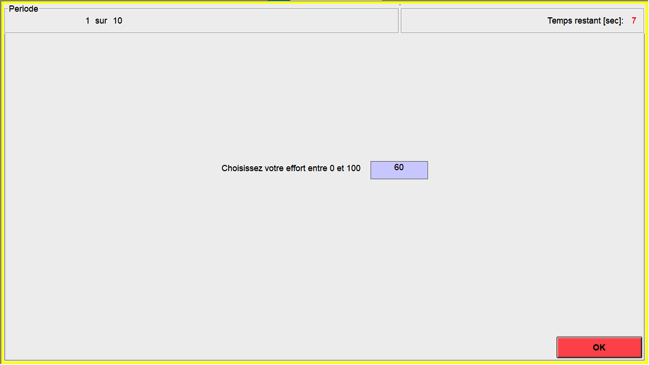
\includegraphics[width = 0.9\textwidth]{05_fig1-annexII.png}

\vspace{0,2cm}
Validez votre choix en cliquant sur «OK». Vous passez à la suite quand
tous les joueurs de votre groupe ont validé leur choix.

\vspace{0,3cm}
\ul{Information sur la somme et la moyenne des efforts des autres
joueurs de votre groupe}

\vspace{0,2cm}
L'écran suivant affiche la somme et la moyenne des efforts choisis par
les trois autres joueurs de votre groupe. L'écran ci-dessous montre un
exemple où la somme des efforts choisis par les trois autres joueurs de
votre groupe est de 140, soit un effort moyen de 140/3~=~46,67 de la
part des trois autres joueurs de votre groupe.

\vspace{0,2cm}
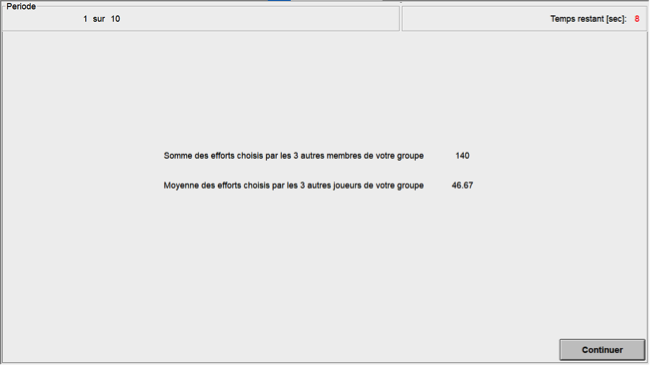
\includegraphics[width = 0.9\textwidth]{05_fig2-annexII.png}
\vspace{0,2cm}

Cliquez sur «Continuer» pour passer à la suite.

\vspace{0,3cm}
\ul{Calcul de votre gain pour la période}

\vspace{0,2cm}
\emph{Votre revenu de production}

\vspace{0,2cm}
Dès que vous-même et les autres joueurs de votre groupe avez validé vos
choix d'effort, l'ordinateur les additionne pour calculer la «Somme des
efforts du groupe». Puis, l'ordinateur tire un nombre entre --~40 et
+~40 au hasard, correspondant à un «Choc aléatoire» qui affecte la
production du groupe. Chaque nombre entre --~40 et +~40 a une même
chance d'être tiré. La «Somme des efforts du groupe» plus ce choc
aléatoire est la «Production totale du groupe», multipliée par 1,5
pour donner le «Revenu total du groupe». Le «Revenu de production»
de chaque joueur vaut un quart du revenu total du groupe.

Par exemple, si vous choisissez un effort de 60 et que la somme des
efforts des autres joueurs de votre groupe est de 140, alors la somme
des efforts du groupe vaut 60~+~140~=~200. Si le choc aléatoire est de
--~40, la production totale du groupe vaut 200~--~40~=~160, le revenu
total du groupe 1,5~×~160~=~240 et votre revenu de production, de même
que celui des trois autres joueurs du groupe, vaut 240/4 =~60.

L'expression de votre revenu de production est~:
\begin{center}
\noindent\fbox{\parbox{\linewidth-2\fboxrule-2\fboxsep}{\centering{Revenu de production \par
=~[1,5~×~(Somme des efforts du groupe~+~Choc aléatoire entre --~40 et
+~40)~/~4]}}}
\end{center}

Votre revenu de production est calculé par l'ordinateur.
\vspace{0,2cm}

\emph{Votre coût de production}

\vspace{0,2cm}
À l'effort que vous choisissez correspond un coût de production, donné
dans le tableau~A ci-dessous.

\newpage

{\centering Tableau A.\par}

{\tabletextsize
\begin{longtable}[]{@{}
  >{\centering\arraybackslash}p{(\columnwidth - 10\tabcolsep) * \real{0.1358}}
  >{\centering\arraybackslash}p{(\columnwidth - 10\tabcolsep) * \real{0.1975}}|
  >{\centering\arraybackslash}p{(\columnwidth - 10\tabcolsep) * \real{0.1358}}
  >{\centering\arraybackslash}p{(\columnwidth - 10\tabcolsep) * \real{0.1975}}|
  >{\centering\arraybackslash}p{(\columnwidth - 10\tabcolsep) * \real{0.1358}}
  >{\centering\arraybackslash}p{(\columnwidth - 10\tabcolsep) * \real{0.1975}}@{}}
\toprule
\begin{minipage}[b]{\linewidth}\centering
Effort choisi
\end{minipage} & \begin{minipage}[b]{\linewidth}\centering
Coût de production
\end{minipage} & \begin{minipage}[b]{\linewidth}\centering
Effort choisi
\end{minipage} & \begin{minipage}[b]{\linewidth}\centering
Coût de production
\end{minipage} & \begin{minipage}[b]{\linewidth}\centering
Effort choisi
\end{minipage} & \begin{minipage}[b]{\linewidth}\centering
Coût de production
\end{minipage} \\
\midrule
0 & 0,00 & 34 & 11,56 & 68 & 46,24 \\
1 & 0,01 & 35 & 12,25 & 69 & 47,61 \\
2 & 0,04 & 36 & 12,96 & 70 & 49,00 \\
3 & 0,09 & 37 & 13,69 & 71 & 50,41 \\
4 & 0,16 & 38 & 14,44 & 72 & 51,84 \\
5 & 0,25 & 39 & 15,21 & 73 & 53,29 \\
6 & 0,36 & 40 & 16,00 & 74 & 54,76 \\
7 & 0,49 & 41 & 16,81 & 75 & 56,25 \\
8 & 0,64 & 42 & 17,64 & 76 & 57,76 \\
9 & 0,81 & 43 & 18,49 & 77 & 59,29 \\
10 & 1,00 & 44 & 19,36 & 78 & 60,84 \\
11 & 1,21 & 45 & 20,25 & 79 & 62,41 \\
12 & 1,44 & 46 & 21,16 & 80 & 64,00 \\
13 & 1,69 & 47 & 22,09 & 81 & 65,61 \\
14 & 1,96 & 48 & 23,04 & 82 & 67,24 \\
15 & 2,25 & 49 & 24,01 & 83 & 68,89 \\
16 & 2,56 & 50 & 25,00 & 84 & 70,56 \\
17 & 2,89 & 51 & 26,01 & 85 & 72,25 \\
18 & 3,24 & 52 & 27,04 & 86 & 73,96 \\
19 & 3,61 & 53 & 28,09 & 87 & 75,69 \\
20 & 4,00 & 54 & 29,16 & 88 & 77,44 \\
21 & 4,41 & 55 & 30,25 & 89 & 79,21 \\
22 & 4,84 & 56 & 31,36 & 90 & 81,00 \\
23 & 5,29 & 57 & 32,49 & 91 & 82,81 \\
24 & 5,76 & 58 & 33,64 & 92 & 84,64 \\
25 & 6,25 & 59 & 34,81 & 93 & 86,49 \\
26 & 6,76 & 60 & 36,00 & 94 & 88,36 \\
27 & 7,29 & 61 & 37,21 & 95 & 90,25 \\
28 & 7,84 & 62 & 38,44 & 96 & 92,16 \\
29 & 8,41 & 63 & 39,69 & 97 & 94,09 \\
30 & 9,00 & 64 & 40,96 & 98 & 96,04 \\
31 & 9,61 & 65 & 42,25 & 99 & 98,01 \\
32 & 10,24 & 66 & 43,56 & 100 & 100,00 \\
33 & 10,89 & 67 & 44,89 & ~ & ~ \\
\bottomrule
\end{longtable}
}

Par exemple, un effort de 10 vous coûte 1~jeton, un effort de 50,
25~jetons, un effort de 100, 100~jetons. Le coût croît plus que
proportionnellement avec l'effort. Ainsi, un effort de 100 coûte plus du
double du coût d'un effort de 50. En résumé~:

\begin{center}
\noindent\fbox{\parbox{\linewidth-2\fboxrule-2\fboxsep}{\centering{Coût de production~=~Coût associé dans le tableau~A à l'effort choisi}}}
\end{center}

Par exemple, un effort de 60 coûte 36~jetons.
\vspace{0,2cm}

\emph{Votre gain pour la période}

\vspace{0,2cm}
Votre gain de production égale votre revenu de production moins votre
coût de production. Votre gain pour la période vaut la somme de ce gain
de production et d'une dotation additionnelle de 10~jetons. En reprenant
les formules précédentes on obtient~:

\begin{center}
\noindent\fbox{\parbox{\linewidth-2\fboxrule-2\fboxsep}{\centering{Gain pour la période
=~Gain de production~+~10
=~Revenu de production~--~Coût de production~+~10
=~[(1,5~×~(Somme des efforts du groupe~+~Choc aléatoire entre --~40 et
+~40)~/~4)
--~Coût de production]~+~10}}}
\end{center}

À noter que votre gain de production est toujours positif ou nul, car si
votre coût de production dépasse votre revenu de production, votre gain
de production est fixé à zéro par l'ordinateur. De ce fait, votre gain
pour la période est toujours supérieur ou égal à 10, du fait de votre
dotation additionnelle de 10~jetons.

Dans l'exemple précédent où vous choisissez un effort de 60 et votre
revenu de production égale aussi 60, votre coût de production vaut 36
d'après le tableau~A, et votre gain de production 60~--~36~=~24~jetons.
En ajoutant 10~jetons additionnels, votre gain pour la période est de
34~jetons.

Votre gain pour la période est calculé par l'ordinateur et restitué à
l'écran~:
\vspace{0,2cm}

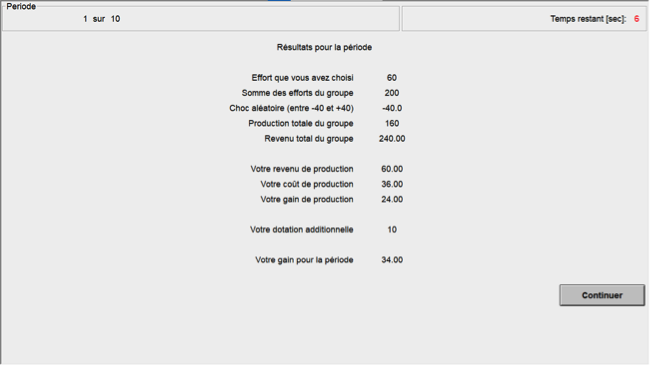
\includegraphics[width = 0.9\textwidth]{05_fig3-annexII.png}

\vspace{0,2cm}
Cliquez sur «Continuer» pour passer à la suite.

\vspace{0,3cm}

\ul{Calcul de votre gain pour l'ensemble de l'expérience}

\vspace{0,2cm}
Votre gain total en jetons pour l'ensemble de l'expérience est égal à la
somme de vos gains pour chacune des 10~périodes de l'expérience. À la
fin du jeu apparaît un écran de synthèse vous indiquant pour les
10~périodes votre gain pour chaque période et le cumul des gains de la
période et des périodes précédentes. Le cumul de vos gains à l'issue de
la dixième période correspond à votre gain total en jetons à l'issue de
l'expérience.

\subsection{Instructions pour le traitement Pression des pairs}

Vous participez à une expérience économique financée par le Centre de
recherches en économie et management de l'Université de Rennes~1. Vous
gagnerez une somme d'argent dont le montant dépendra des décisions que
vous prendrez et des décisions que prendront les autres joueurs.

Il est interdit de communiquer avec d'autres joueurs sous peine
d'exclusion de la session et des gains. Si vous avez des questions,
levez la main. Nous y répondrons en privé.

Durant l'expérience, vos gains sont calculés en jetons. À la fin de
l'expérience, votre gain total en jetons est converti en euros au taux
de 1~euro~=~45~jetons.

À votre gain en jetons converti en euros s'ajoute un forfait de 4~euros.
Vos gains vous sont payés à la fin de l'expérience. Vous seul êtes
informé de la somme que vous avez gagnée.

Au début de l'expérience, les joueurs sont répartis en groupes de
quatre, tirés au hasard. Vous êtes donc avec trois autres joueurs. Ce
groupe correspond à une équipe de production. Vous ne savez pas quels
joueurs font partie de votre groupe. L'expérience consiste en
10~périodes rémunérées. Toutes les périodes sont identiques. Les groupes
restent inchangés durant l'expérience.

Chaque période comprend deux étapes. Ces instructions présentent le
déroulement de la première étape, puis celui de la seconde.
\vspace{0,2cm}

• Première étape

\vspace{0,2cm}
Au début de la première étape apparaît un écran où vous devez choisir un
niveau d'effort, sous la forme d'un nombre compris entre 0 et 100,
représentant votre contribution à la production de votre groupe. Dans
l'exemple d'écran ci-dessous, un effort de 60 est choisi.

\vspace{0,2cm}

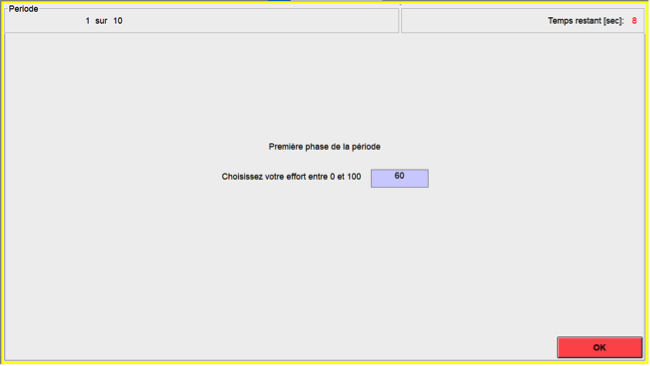
\includegraphics[width = 0.9\textwidth]{05_fig4-annexII.png}

Validez votre choix en cliquant sur «OK». Vous passez à la suite quand
tous les joueurs de votre groupe ont validé leur choix.
\vspace{0,3cm}

\newpage

\ul{Information sur les efforts des autres joueurs}

\vspace{0,2cm}
L'écran suivant affiche les efforts choisis par les autres joueurs de
votre groupe dans un ordre aléatoire qui change à chaque période.
L'écran ci-dessous, montre un exemple où ces trois autres joueurs ont
choisi des efforts de 20, 40 et 80.

\vspace{0,2cm}

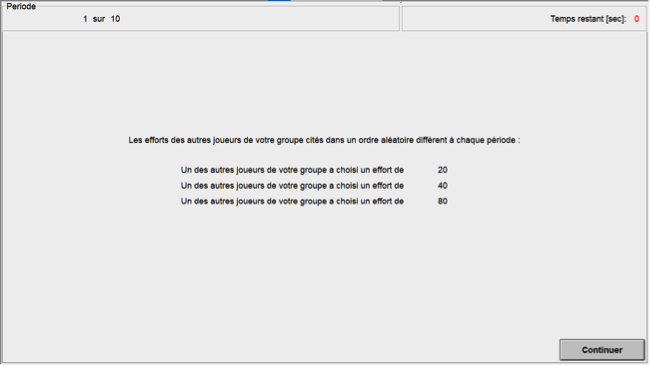
\includegraphics[width = 0.9\textwidth]{05_fig5-annexII.png}

Cliquez sur «Continuer» pour passer à la suite.
\vspace{0,3cm}

\ul{Calcul de votre gain initial après la première étape}

\vspace{0,2cm}

\emph{Votre revenu de production}

\vspace{0,2cm}
Dès que vous-même et les autres joueurs de votre groupe avez validé vos
choix d'effort, l'ordinateur les additionne pour calculer la «Somme des
efforts du groupe». Puis, l'ordinateur tire un nombre entre --~40 et
+~40 au hasard, correspondant à un «Choc aléatoire» qui affecte la
production du groupe. Chaque nombre entre --~40 et +~40 a une même
chance d'être tiré. La «Somme des efforts du groupe» plus ce choc
aléatoire est la «Production totale du groupe», multipliée par 1,5
pour donner le «Revenu total du groupe». Le «Revenu de production»
de chaque joueur vaut un quart du revenu total du groupe.

Par exemple, si vous choisissez un effort de 60 et que la somme des
efforts des autres joueurs de votre groupe est de 140, alors la somme
des efforts du groupe vaut 60~+~140~=~200. Si le choc aléatoire est de
--~40, la production totale du groupe vaut 200~--~40~=~160, le revenu
total du groupe 1,5~×~160~=~240 et votre revenu de production, de même
que celui des trois autres joueurs du groupe, vaut 240/4 =~60.

L'expression de votre revenu de production est~:
\begin{center}
\noindent\fbox{\parbox{\linewidth-2\fboxrule-2\fboxsep}{\centering{Revenu de production \par
=~[1,5~×~(Somme des efforts du groupe~+~Choc aléatoire entre --~40 et
+~40)~/~4]}}}
\end{center}

Votre revenu de production est calculé par l'ordinateur.
\vspace{0,2cm}

\emph{Votre coût de production}

\vspace{0,2cm}
À l'effort que vous choisissez correspond un coût de production, donné
dans le tableau~A ci-dessous.

\vspace{0,2cm}
{\centering Tableau A.\par}

{\tabletextsize
\begin{longtable}[]{@{}
  >{\centering\arraybackslash}p{(\columnwidth - 10\tabcolsep) * \real{0.1358}}
  >{\centering\arraybackslash}p{(\columnwidth - 10\tabcolsep) * \real{0.1975}}|
  >{\centering\arraybackslash}p{(\columnwidth - 10\tabcolsep) * \real{0.1358}}
  >{\centering\arraybackslash}p{(\columnwidth - 10\tabcolsep) * \real{0.1975}}|
  >{\centering\arraybackslash}p{(\columnwidth - 10\tabcolsep) * \real{0.1358}}
  >{\centering\arraybackslash}p{(\columnwidth - 10\tabcolsep) * \real{0.1975}}@{}}
\toprule
\begin{minipage}[b]{\linewidth}\centering
Effort choisi
\end{minipage} & \begin{minipage}[b]{\linewidth}\centering
Coût de production
\end{minipage} & \begin{minipage}[b]{\linewidth}\centering
Effort choisi
\end{minipage} & \begin{minipage}[b]{\linewidth}\centering
Coût de production
\end{minipage} & \begin{minipage}[b]{\linewidth}\centering
Effort choisi
\end{minipage} & \begin{minipage}[b]{\linewidth}\centering
Coût de production
\end{minipage} \\
\midrule
\endhead
\bottomrule
\endlastfoot
0 & 0,00 & 34 & 11,56 & 68 & 46,24 \\
1 & 0,01 & 35 & 12,25 & 69 & 47,61 \\
2 & 0,04 & 36 & 12,96 & 70 & 49,00 \\
3 & 0,09 & 37 & 13,69 & 71 & 50,41 \\
4 & 0,16 & 38 & 14,44 & 72 & 51,84 \\
5 & 0,25 & 39 & 15,21 & 73 & 53,29 \\
6 & 0,36 & 40 & 16,00 & 74 & 54,76 \\
7 & 0,49 & 41 & 16,81 & 75 & 56,25 \\
8 & 0,64 & 42 & 17,64 & 76 & 57,76 \\
9 & 0,81 & 43 & 18,49 & 77 & 59,29 \\
10 & 1,00 & 44 & 19,36 & 78 & 60,84 \\
11 & 1,21 & 45 & 20,25 & 79 & 62,41 \\
12 & 1,44 & 46 & 21,16 & 80 & 64,00 \\
13 & 1,69 & 47 & 22,09 & 81 & 65,61 \\
14 & 1,96 & 48 & 23,04 & 82 & 67,24 \\
15 & 2,25 & 49 & 24,01 & 83 & 68,89 \\
16 & 2,56 & 50 & 25,00 & 84 & 70,56 \\
17 & 2,89 & 51 & 26,01 & 85 & 72,25 \\
18 & 3,24 & 52 & 27,04 & 86 & 73,96 \\
19 & 3,61 & 53 & 28,09 & 87 & 75,69 \\
20 & 4,00 & 54 & 29,16 & 88 & 77,44 \\
21 & 4,41 & 55 & 30,25 & 89 & 79,21 \\
22 & 4,84 & 56 & 31,36 & 90 & 81,00 \\
23 & 5,29 & 57 & 32,49 & 91 & 82,81 \\
24 & 5,76 & 58 & 33,64 & 92 & 84,64 \\
25 & 6,25 & 59 & 34,81 & 93 & 86,49 \\
26 & 6,76 & 60 & 36,00 & 94 & 88,36 \\
27 & 7,29 & 61 & 37,21 & 95 & 90,25 \\
28 & 7,84 & 62 & 38,44 & 96 & 92,16 \\
29 & 8,41 & 63 & 39,69 & 97 & 94,09 \\
30 & 9,00 & 64 & 40,96 & 98 & 96,04 \\
31 & 9,61 & 65 & 42,25 & 99 & 98,01 \\
32 & 10,24 & 66 & 43,56 & 100 & 100,00 \\
33 & 10,89 & 67 & 44,89 & ~ & ~ \\
\end{longtable}
}

Par exemple, un effort de 10 vous coûte 1 jeton, un effort de 50,
25~jetons, un effort de 100, 100~jetons. Le coût croît plus que
proportionnellement avec l'effort. Ainsi, un effort de 100 coûte plus du
double du coût d'un effort de 50. En résumé~:

\begin{center}
\noindent\fbox{\parbox{\linewidth-2\fboxrule-2\fboxsep}{\centering{Coût de production~=~Coût associé dans le tableau~A à l'effort choisi}}}
\end{center}

Par exemple, un effort de 60 coûte 36~jetons.

\vspace{0,2cm}
\emph{Votre gain initial après la première étape}

\vspace{0,2cm}
Votre gain de production égale votre revenu de production moins votre
coût de production. Votre gain initial à l'issue de la première étape
vaut la somme de ce gain de production et d'une dotation additionnelle
de 10~jetons. En reprenant les formules précédentes on obtient~:

\begin{center}
\noindent\fbox{\parbox{\linewidth-2\fboxrule-2\fboxsep}{\centering{Gain pour la période
=~Gain de production~+~10
=~Revenu de production~--~Coût de production~+~10
=~[(1,5~×~(Somme des efforts du groupe~+~Choc aléatoire entre --~40 et
+~40)~/~4)
--~Coût de production]~+~10}}}
\end{center}

À noter que votre gain de production est toujours positif ou nul, car si
votre coût de production dépasse votre revenu de production, votre gain
de production est fixé à zéro par l'ordinateur. De ce fait, votre gain
initial après la première étape est toujours supérieur ou égal à 10, du
fait de votre dotation additionnelle de 10~jetons.

Dans l'exemple précédent où vous choisissez un effort de 60 et votre
revenu de production égale aussi 60, votre coût de production vaut 36
d'après le tableau~A, et votre gain de production 60~--~36~=~24~jetons.
En ajoutant 10~jetons additionnels, votre gain pour la période est de
34~jetons.

Votre gain initial après la première étape est calculé par l'ordinateur
et restitué à l'écran~:

\vspace{0,2cm}

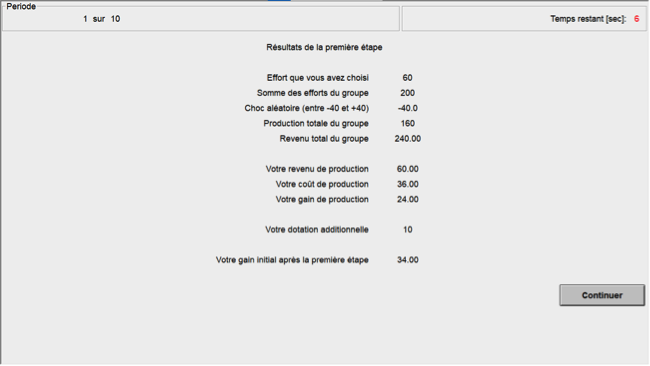
\includegraphics[width = 0.9\textwidth]{05_fig6-annexII.png}

Cliquez sur «Continuer» pour passer à la suite.
\vspace{0,2cm}

•~~Seconde étape

\vspace{0,2cm}
Dans cette seconde étape, vous, comme les autres joueurs du groupe,
pouvez utiliser tout ou partie de vos 10~jetons additionnels pour
réduire les gains des trois autres joueurs de votre groupe en leur
attribuant des points de désapprobation.

Un écran apparaît où vous devez saisir les points de désapprobation que
vous attribuez aux autres joueurs de votre groupe, comme dans l'exemple
ci-dessous~:

\vspace{0,2cm}

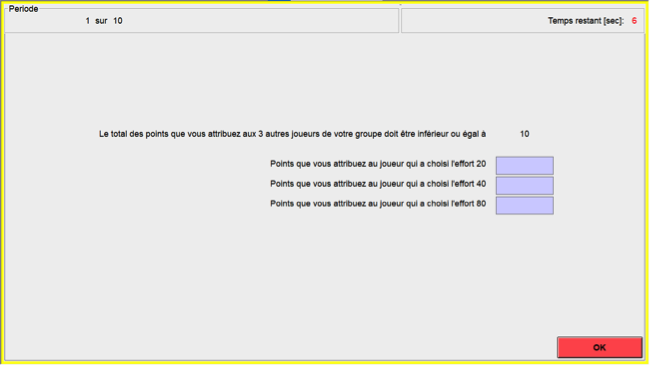
\includegraphics[width = 0.9\textwidth]{05_fig7-annexII.png}

L'ordre d'affichage des efforts des autres joueurs est aléatoire et
varie d'une période à l'autre. C'est donc sur la seule base des efforts
choisis lors de la première étape de cette période que vous décidez des
points que vous leur attribuez. Le nombre total de points attribués aux
trois autres joueurs doit être inférieur ou égal à 10. Validez votre
choix en cliquant sur «OK».
\vspace{0,2cm}

\ul{Gains à l'issue de la seconde étape}

\vspace{0,2cm}
Vous réduisez le gain des autres joueurs du triple du nombre de points
de désapprobation que vous leur attribuez. Si vous attribuez 0~point à
un joueur, vous ne changez pas son gain, si vous lui attribuez 1~point,
vous réduisez son gain de 3~jetons, de 6~jetons si vous lui attribuez
2~points et ainsi de suite.

Attribuer des points aux autres joueurs vous coûte en jetons le total
des points que vous attribuez, ce total ne pouvant dépasser 10~jetons.
Par exemple, attribuer 2~points à chacun des trois autres joueurs vous
coûte 6~jetons. Vous ne pourriez attribuer 5~points à chacun des trois
autres joueurs car cela représenterait 15~points, au-dessus du maximum
de 10.

Votre gain est aussi diminué du triple de nombre total de points de
désapprobation que vous recevez de la part des autres joueurs. Si vous
recevez 0~point, votre gain est inchangé, si vous recevez 1~point, il
baisse de 3~jetons, si vous recevez 2~points, il baisse de 6~jetons,
etc.

Par exemple, si votre gain initial à l'issue de la première étape est de
34~jetons, et si lors de la seconde étape vous attribuez 2~points à
chacun des trois autres joueurs, et si vous recevez des autres joueurs
3~points au total, votre gain final sera de
34~--~3~×~2~--~3~×~3~=~19~jetons.

Plus généralement, votre gain pour la période est calculé de la façon
suivante~:

\begin{center}
\noindent\fbox{\parbox{\linewidth-2\fboxrule-2\fboxsep}{\centering{Gain pour la période
=~Gain initial~--~Nombre total de points attribué~--~3~×~Nombre total de
points reçus}}}
\end{center}

Les points que vous recevez peuvent annuler votre gain mais non le
rendre négatif~: si votre nombre de points reçus dépasse le tiers de
votre gain initial moins le nombre de points que vous attribuez, alors
votre gain pour la période sera considéré comme nul.

Le calcul est fait par l'ordinateur et affiché à l'écran~:

\vspace{0,2cm}

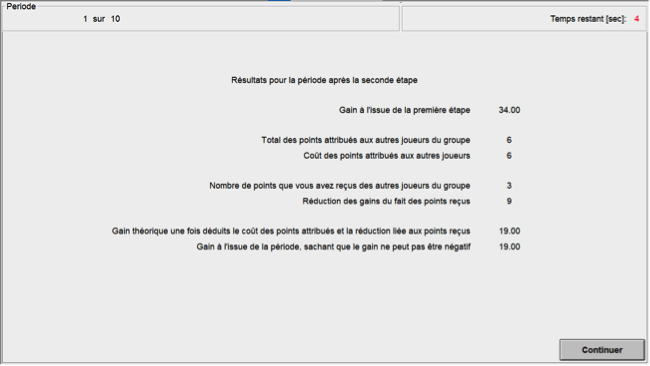
\includegraphics[width = 0.9\textwidth]{05_fig8-annexII.png}

Cliquez sur «Continuer» pour passer à la suite.
\vspace{0,2cm}

\ul{Calcul de votre gain pour l'ensemble de l'expérience}

\vspace{0,2cm}
Votre gain total en jetons pour l'ensemble de l'expérience égale la
somme de vos gains pour chacune des 10~périodes de l'expérience. À la
fin du jeu apparaît un écran de synthèse vous indiquant pour les
10~périodes votre gain pour chaque période et le cumul des gains de la
période et des périodes précédentes. Le cumul de vos gains à l'issue de
la dixième période correspond à votre gain total en jetons à l'issue de
l'expérience.

\subsection{Instructions pour le traitement Objectif d'équipe}

Vous participez à une expérience économique financée par le Centre de
recherches en économie et management de l'Université de Rennes~1. Vous
gagnerez une somme d'argent dont le montant dépendra des décisions que
vous prendrez et des décisions que prendront les autres joueurs.

Il est interdit de communiquer avec d'autres joueurs sous peine
d'exclusion de la session et des gains. Si vous avez des questions,
levez la main. Nous y répondrons en privé.

Durant l'expérience, vos gains sont calculés en jetons. À la fin de
l'expérience, votre gain total en jetons est converti en euros au taux
de 1~euro~=~45~jetons.

À votre gain en jetons converti en euros s'ajoute un forfait de 4~euros.
Vos gains vous sont payés à la fin de l'expérience. Vous seul êtes
informé de la somme que vous avez gagnée.

Au début de l'expérience, les joueurs sont répartis en groupes de
quatre, tirés au hasard. Vous êtes donc avec trois autres joueurs. Ce
groupe correspond à une équipe de production. Vous ne savez pas quels
joueurs font partie de votre groupe. L'expérience consiste en
10~périodes rémunérées. Toutes les périodes sont identiques. Les groupes
restent inchangés durant l'expérience.

Au début de chaque période apparaît un écran où vous devez choisir un
niveau d'effort, sous la forme d'un nombre compris entre 0 et 100,
représentant votre contribution à la production de votre groupe. Dans
l'exemple d'écran ci-dessous, un effort de 60 est choisi.

\vspace{0,2cm}

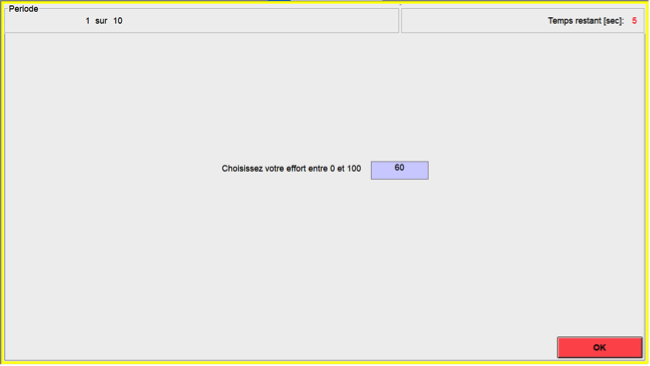
\includegraphics[width = 0.9\textwidth]{05_fig9-annexII.png}

Validez votre choix en cliquant sur «OK». Vous passez à la suite quand
tous les joueurs de votre groupe ont validé leur choix.
\vspace{0,2cm}

\ul{Information sur les efforts des autres joueurs}

\vspace{0,2cm}
L'écran suivant affiche les efforts choisis par les autres joueurs de
votre groupe dans un ordre aléatoire qui change à chaque période.
L'écran ci-dessous montre un exemple où ces trois autres joueurs ont
choisi des efforts de 20, 40 et 80.

\vspace{0,2cm}

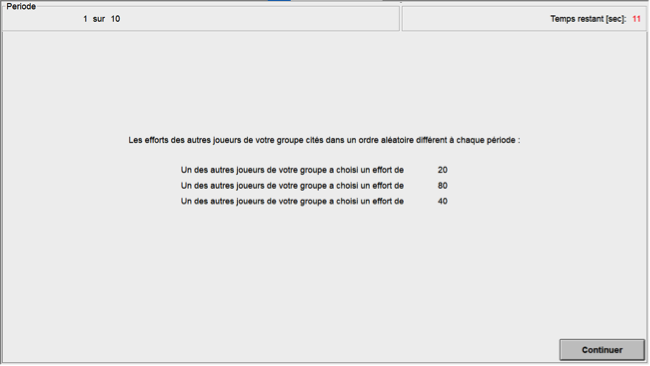
\includegraphics[width = 0.9\textwidth]{05_fig10-annexII.png}

Cliquez sur «Continuer» pour passer à la suite.
\vspace{0,2cm}

\ul{Calcul de votre gain pour la période}

\vspace{0,2cm}
\emph{Votre revenu de production}

\vspace{0,2cm}
Dès que vous-même et les autres joueurs de votre groupe avez validé vos
choix d'effort, l'ordinateur les additionne pour calculer la «Somme des
efforts du groupe». Puis, l'ordinateur tire un nombre entre --~40 et
+~40 au hasard, correspondant à un «Choc aléatoire» qui affecte la
production du groupe. Chaque nombre entre --~40 et +~40 a une même
chance d'être tiré. La «Somme des efforts du groupe» plus ce choc
aléatoire est la «Production totale du groupe», multipliée par 1,5
pour donner le «Revenu total du groupe». Le «Revenu de production»
de chaque joueur vaut un quart du revenu total du groupe.

Si le revenu total du groupe est supérieur ou égal à un seuil fixé à
450~jetons, alors votre revenu de production est égal au quart du revenu
total du groupe. Sinon, votre revenu de production égale un montant
minimal fixe de 7,5~jetons.

Par exemple, si vous choisissez un effort de 60 et les autres joueurs de
votre groupe 20, 40 et 80, la somme des efforts du groupe vaut
60~+~20~+~40~+~80~=~200. Si le choc aléatoire est de --~40, la
production totale du groupe vaut 200~--~40~=~160 et le revenu total du
groupe 1,5~×~160~=~240. Le revenu total du groupe étant inférieur au
seuil de 450, votre revenu de production, de même que celui des trois
autres joueurs du groupe, vaut 7,5~jetons.

Si vous choisissez toujours un effort de 60 mais les autres joueurs de
votre groupe 40, 80 et 100, la somme des efforts du groupe vaut
60~+~40~+~80~+~100~=~280. Si le choc aléatoire est cette fois de +~40,
la production totale du groupe vaut 280~+~40~=~320 et le revenu total du
groupe 1,5~×~320~=~480. Le revenu total du groupe étant supérieur au
seuil de 450, votre revenu de production, de même que celui des trois
autres joueurs du groupe, vaut 480/4~=~120~jetons.

L'expression de votre revenu de production est~:

\begin{center}
\noindent\fbox{\parbox{\linewidth-2\fboxrule-2\fboxsep}{\centering{
    \emph{Si le revenu total du groupe est supérieur ou égal à 450, alors~:}

\vspace{.2cm}

Revenu de production
=~[1,5~×~(Somme des efforts du groupe~+~Choc aléatoire entre --~40 et
+~40)/4]

\vspace{.2cm}

\emph{Si le revenu total du groupe est inférieur à 450, alors~:}

\vspace{.2cm}

Revenu de production~=~7,5
Votre revenu de production est calculé par l'ordinateur.}}}
\end{center}

\emph{Votre coût de production}

\vspace{0,2cm}
À l'effort que vous choisissez correspond un coût de production, donné
dans le tableau~A ci-dessous.

\vspace{0,2cm}
{\centering Tableau A.\par}

{\tabletextsize
\begin{longtable}[]{@{}
  >{\centering\arraybackslash}p{(\columnwidth - 10\tabcolsep) * \real{0.1358}}
  >{\centering\arraybackslash}p{(\columnwidth - 10\tabcolsep) * \real{0.1975}}|
  >{\centering\arraybackslash}p{(\columnwidth - 10\tabcolsep) * \real{0.1358}}
  >{\centering\arraybackslash}p{(\columnwidth - 10\tabcolsep) * \real{0.1975}}|
  >{\centering\arraybackslash}p{(\columnwidth - 10\tabcolsep) * \real{0.1358}}
  >{\centering\arraybackslash}p{(\columnwidth - 10\tabcolsep) * \real{0.1975}}@{}}
\toprule
\begin{minipage}[b]{\linewidth}\centering
Effort choisi
\end{minipage} & \begin{minipage}[b]{\linewidth}\centering
Coût de production
\end{minipage} & \begin{minipage}[b]{\linewidth}\centering
Effort choisi
\end{minipage} & \begin{minipage}[b]{\linewidth}\centering
Coût de production
\end{minipage} & \begin{minipage}[b]{\linewidth}\centering
Effort choisi
\end{minipage} & \begin{minipage}[b]{\linewidth}\centering
Coût de production
\end{minipage} \\
\midrule
\endhead
\bottomrule
\endlastfoot
0 & 0,00 & 34 & 11,56 & 68 & 46,24 \\
1 & 0,01 & 35 & 12,25 & 69 & 47,61 \\
2 & 0,04 & 36 & 12,96 & 70 & 49,00 \\
3 & 0,09 & 37 & 13,69 & 71 & 50,41 \\
4 & 0,16 & 38 & 14,44 & 72 & 51,84 \\
5 & 0,25 & 39 & 15,21 & 73 & 53,29 \\
6 & 0,36 & 40 & 16,00 & 74 & 54,76 \\
7 & 0,49 & 41 & 16,81 & 75 & 56,25 \\
8 & 0,64 & 42 & 17,64 & 76 & 57,76 \\
9 & 0,81 & 43 & 18,49 & 77 & 59,29 \\
10 & 1,00 & 44 & 19,36 & 78 & 60,84 \\
11 & 1,21 & 45 & 20,25 & 79 & 62,41 \\
12 & 1,44 & 46 & 21,16 & 80 & 64,00 \\
13 & 1,69 & 47 & 22,09 & 81 & 65,61 \\
14 & 1,96 & 48 & 23,04 & 82 & 67,24 \\
15 & 2,25 & 49 & 24,01 & 83 & 68,89 \\
16 & 2,56 & 50 & 25,00 & 84 & 70,56 \\
17 & 2,89 & 51 & 26,01 & 85 & 72,25 \\
18 & 3,24 & 52 & 27,04 & 86 & 73,96 \\
19 & 3,61 & 53 & 28,09 & 87 & 75,69 \\
20 & 4,00 & 54 & 29,16 & 88 & 77,44 \\
21 & 4,41 & 55 & 30,25 & 89 & 79,21 \\
22 & 4,84 & 56 & 31,36 & 90 & 81,00 \\
23 & 5,29 & 57 & 32,49 & 91 & 82,81 \\
24 & 5,76 & 58 & 33,64 & 92 & 84,64 \\
25 & 6,25 & 59 & 34,81 & 93 & 86,49 \\
26 & 6,76 & 60 & 36,00 & 94 & 88,36 \\
27 & 7,29 & 61 & 37,21 & 95 & 90,25 \\
28 & 7,84 & 62 & 38,44 & 96 & 92,16 \\
29 & 8,41 & 63 & 39,69 & 97 & 94,09 \\
30 & 9,00 & 64 & 40,96 & 98 & 96,04 \\
31 & 9,61 & 65 & 42,25 & 99 & 98,01 \\
32 & 10,24 & 66 & 43,56 & 100 & 100,00 \\
33 & 10,89 & 67 & 44,89 & ~ & ~ \\
\end{longtable}
}

Par exemple, un effort de 10 vous coûte 1~jeton, un effort de 50,
25~jetons, un effort de 100, 100~jetons. Le coût croît plus que
proportionnellement avec l'effort. Ainsi, un effort de 100 coûte plus du
double du coût d'un effort de 50. En résumé~:

\begin{center}
\noindent\fbox{\parbox{\linewidth-2\fboxrule-2\fboxsep}{\centering{Coût de production~=~Coût associé dans le tableau~A à l'effort choisi}}}
\end{center}

Par exemple, un effort de 60 coûte 36~jetons.
\vspace{.2cm}

\emph{Votre gain pour la période}

\vspace{.2cm}
Votre gain de production égale votre revenu de production moins votre
coût de production. Votre gain pour la période vaut la somme de ce gain
de production et d'une dotation additionnelle de 10~jetons. En reprenant
les formules précédentes on obtient~:

\newpage

\begin{center}
\noindent\fbox{\parbox{\linewidth-2\fboxrule-2\fboxsep}{\centering{
Gain pour la période
=~Gain de production~+~10 \par
=~Revenu de production~--~Coût de production~+~10~=

\vspace{.2cm}
\emph{Si le revenu total du groupe est supérieur ou égal à 450, alors~:}

\vspace{.2cm}
[(1,5~×~(Somme des efforts du groupe~+~Choc aléatoire entre --~40 et
+~40)/4)
--~Coût de production]~+~10

\vspace{.2cm}
\emph{Si le revenu total du groupe est inférieur à 450, alors~:}

\vspace{.2cm}
[7,5~--~Coût de production]~+~10}}}
\end{center}

À noter~: votre gain de production est toujours positif ou nul, car si
votre coût de production dépasse votre revenu de production, votre gain
de production est fixé à zéro par l'ordinateur. De ce fait, votre gain
pour la période est toujours supérieur ou égal à 10, du fait de votre
dotation additionnelle de 10~jetons.

Dans le premier exemple précédent où vous choisissez un effort de 60 et
où le revenu total de votre groupe est égal à 240, en dessous du seuil
de 450, votre revenu de production est fixé à 7,5. Votre coût de
production, égal à 36 d'après le tableau~A, dépasse votre revenu de
production de 7,5. Par suite, l'ordinateur fixe votre gain de production
à 0. En ajoutant 10~jetons additionnels, votre gain pour la période est
de 10~jetons.

Dans le second exemple précédent où vous choisissez toujours un effort
de 60 mais où le revenu total de votre groupe est égal à 480, en dessus
du seuil de 450, votre revenu de production vaut le quart du revenu du
groupe, soit 120. Votre coût de production est égal à 36 d'après le
tableau~A. Par suite, votre gain de production vaut 120~--~36~=~84. En
ajoutant 10~jetons additionnels, votre gain pour la période est de
94~jetons.

Votre gain pour la période est calculé par l'ordinateur et restitué à
l'écran~:

\vspace{0,2cm}

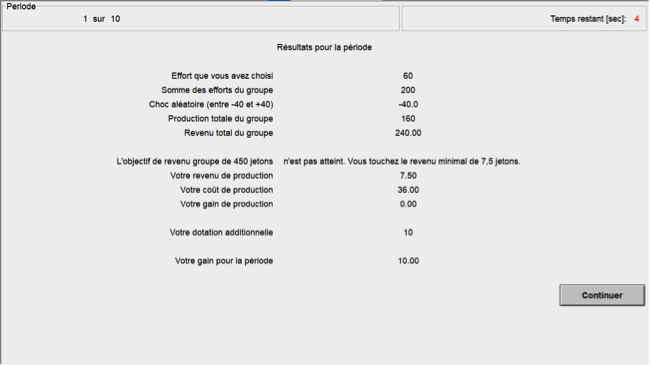
\includegraphics[width = 0.9\textwidth]{05_fig11-annexII.png}

Cliquez sur «Continuer» pour passer à la suite.

\vspace{.2cm}
\ul{Calcul de votre gain pour l'ensemble de l'expérience}

\vspace{.2cm}
Votre gain total en jetons pour l'ensemble de l'expérience égale la
somme de vos gains pour chacune des 10~périodes de l'expérience. À la
fin du jeu apparaît un écran de synthèse vous indiquant pour les
10~périodes votre gain pour chaque période et le cumul des gains de la
période et des périodes précédentes. Le cumul de vos gains à l'issue de
la dixième période correspond à votre gain total en jetons à l'issue de
l'expérience.

\subsection{Instructions pour le traitement Tournois entre équipes}

Vous participez à une expérience économique financée par le Centre de
recherches en économie et management de l'Université de Rennes~1. Vous
gagnerez une somme d'argent dont le montant dépendra des décisions que
vous prendrez et des décisions que prendront les autres joueurs.

Il est interdit de communiquer avec d'autres joueurs sous peine
d'exclusion de la session et des gains. Si vous avez des questions,
levez la main. Nous y répondrons en privé.

Durant l'expérience, vos gains sont calculés en jetons. À la fin de
l'expérience, votre gain total en jetons est converti en euros au taux
de 1~euro~=~45~jetons.

À votre gain en jetons converti en euros s'ajoute un forfait de 4~euros.
Vos gains vous sont payés à la fin de l'expérience. Vous seul êtes
informé de la somme que vous avez gagnée.

Au début de l'expérience, les joueurs sont répartis en groupes de
quatre, tirés au hasard. Vous êtes donc avec trois autres joueurs. Ce
groupe correspond à une équipe de production. Vous ne savez pas quels
joueurs font partie de votre groupe. L'expérience consiste en
10~périodes rémunérées. Toutes les périodes sont identiques. Les groupes
restent inchangés durant l'expérience.

À chaque période, les résultats de votre groupe sont comparés à ceux
d'un groupe concurrent qui reste le même pendant toute l'expérience. Le
groupe vainqueur de cette comparaison reçoit 180~jetons du groupe
vaincu.

Au début de chaque période apparaît un écran où vous devez choisir un
niveau d'effort, sous la forme d'un nombre compris entre 0 et 100,
représentant votre contribution à la production de votre groupe. Dans
l'exemple d'écran ci-dessous, un effort de 60 est choisi.

\vspace{0,2cm}

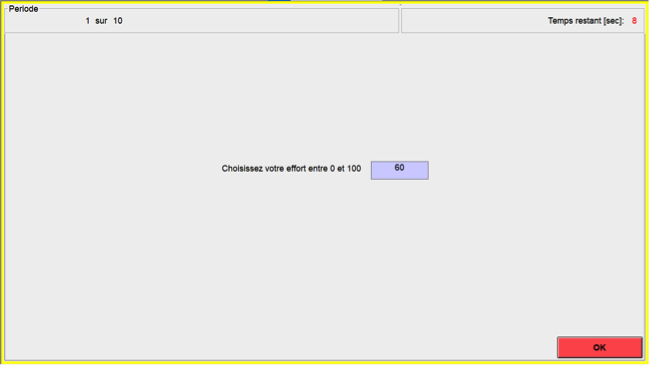
\includegraphics[width = 0.9\textwidth]{05_fig12-annexII.png}

Validez votre choix en cliquant sur «OK». Vous passez à la suite quand
tous les joueurs de votre groupe ont validé leur choix.

\vspace{.2cm}
\ul{Information sur les efforts des autres joueurs}

\vspace{.2cm}
L'écran suivant affiche les efforts choisis par les autres joueurs de
votre groupe dans un ordre aléatoire qui change à chaque période.
L'écran ci-dessous, montre un exemple où ces trois autres joueurs ont
choisi des efforts de 20, 40 et 80.

\vspace{0,2cm}

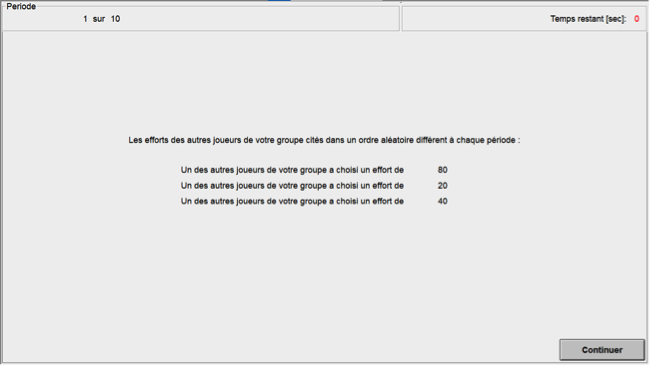
\includegraphics[width = 0.9\textwidth]{05_fig13-annexII.png}

Cliquez sur «Continuer» pour passer à la suite.

\vspace{.2cm}
\ul{Calcul de votre gain pour la période}

\vspace{.2cm}
\emph{Votre revenu de production}

\vspace{.2cm}
Dès que vous-même et les autres joueurs de votre groupe avez validé vos
choix d'effort, l'ordinateur les additionne pour calculer la «Somme des
efforts du groupe». Puis, l'ordinateur tire un nombre entre --~40 et
+~40 au hasard, correspondant à un «Choc aléatoire» qui affecte la
production du groupe. Chaque nombre entre --~40 et +~40 a une même
chance d'être tiré. La «Somme des efforts du groupe» plus ce choc
aléatoire est la «Production totale du groupe», multipliée par 1,5
pour donner le «Revenu total du groupe». Le «Revenu de production»
de chaque joueur vaut un quart du revenu total du groupe.

Le revenu total de votre groupe est comparé à celui du groupe qui est le
concurrent du vôtre pendant toute l'expérience. S'il est supérieur à
celui du concurrent, celui-ci transfère à votre groupe 180~jetons qui
s'ajoutent au revenu total de votre groupe. S'il est inférieur, votre
groupe lui transfère 180~jetons qui se déduisent du revenu total de
votre groupe. En cas d'égalité, aucun transfert n'a lieu.

Le «Revenu de production» de chaque joueur vaut un quart du revenu
total du groupe après transfert.

Par exemple, si vous choisissez un effort de 60 et les autres joueurs de
votre groupe 20, 40 et 80, la somme des efforts du groupe vaut
60~+~20~+~40~+~80~=~200. Si le choc aléatoire est de --~40, la
production totale du groupe vaut 200~--~40~=~160 et le revenu total du
groupe 1,5~×~160~=~240.

Si, dans cet exemple, le groupe concurrent a un revenu total supérieur à
240, donc supérieur au vôtre, votre groupe lui transfère 180~jetons qui
se déduisent du revenu total de votre groupe~: il ne reste donc que
240~--~180~=~60~jetons à répartir entre les quatre joueurs de votre
groupe. D'où pour chacun un revenu individuel de production de
60/4~=~15~jetons.

Si, dans cet exemple, le groupe concurrent a un revenu total inférieur à
240, donc inférieur au vôtre, il transfère à votre groupe 180~jetons qui
s'ajoutent au revenu total de votre groupe~: il y a donc
240~+~180~=~420~jetons à répartir entre les quatre joueurs de votre
groupe. D'où pour chacun un revenu individuel de production de
420/4~=~105~jetons.

L'expression générale de votre revenu de production est la suivante~:

\begin{center}
\noindent\fbox{\parbox{\linewidth-2\fboxrule-2\fboxsep}{\centering{Revenu de production =~[(1,5~×~(Somme des efforts du groupe~+~Choc aléatoire de production
entre --~40 et +~40)~+~180)/4]

\emph{si le revenu total de votre groupe est supérieur à celui du groupe
concurrent}

\vspace{.3cm}
Revenu de production
=~[(1,5~×~(Somme des efforts du groupe~+~Choc aléatoire de production
entre --~40 et +~40)~--~180)/4]

\emph{si le revenu total de votre groupe est inférieur à celui du groupe
concurrent}}}}
\end{center}


\vspace{.2cm}
Votre revenu de production est calculé par l'ordinateur.

\vspace{.3cm}
\emph{Votre coût de production}

\vspace{.2cm}
À l'effort que vous choisissez correspond un coût de production, donné
dans le tableau~A ci-dessous.

\vspace{0,2cm}
{\centering Tableau A.\par}

{\tabletextsize
\begin{longtable}[]{@{}
  >{\centering\arraybackslash}p{(\columnwidth - 10\tabcolsep) * \real{0.1358}}
  >{\centering\arraybackslash}p{(\columnwidth - 10\tabcolsep) * \real{0.1975}}|
  >{\centering\arraybackslash}p{(\columnwidth - 10\tabcolsep) * \real{0.1358}}
  >{\centering\arraybackslash}p{(\columnwidth - 10\tabcolsep) * \real{0.1975}}|
  >{\centering\arraybackslash}p{(\columnwidth - 10\tabcolsep) * \real{0.1358}}
  >{\centering\arraybackslash}p{(\columnwidth - 10\tabcolsep) * \real{0.1975}}@{}}
\toprule
\begin{minipage}[b]{\linewidth}\centering
Effort choisi
\end{minipage} & \begin{minipage}[b]{\linewidth}\centering
Coût de production
\end{minipage} & \begin{minipage}[b]{\linewidth}\centering
Effort choisi
\end{minipage} & \begin{minipage}[b]{\linewidth}\centering
Coût de production
\end{minipage} & \begin{minipage}[b]{\linewidth}\centering
Effort choisi
\end{minipage} & \begin{minipage}[b]{\linewidth}\centering
Coût de production
\end{minipage} \\
\midrule
\endhead
\bottomrule
\endlastfoot
0 & 0,00 & 34 & 11,56 & 68 & 46,24 \\
1 & 0,01 & 35 & 12,25 & 69 & 47,61 \\
2 & 0,04 & 36 & 12,96 & 70 & 49,00 \\
3 & 0,09 & 37 & 13,69 & 71 & 50,41 \\
4 & 0,16 & 38 & 14,44 & 72 & 51,84 \\
5 & 0,25 & 39 & 15,21 & 73 & 53,29 \\
6 & 0,36 & 40 & 16,00 & 74 & 54,76 \\
7 & 0,49 & 41 & 16,81 & 75 & 56,25 \\
8 & 0,64 & 42 & 17,64 & 76 & 57,76 \\
9 & 0,81 & 43 & 18,49 & 77 & 59,29 \\
10 & 1,00 & 44 & 19,36 & 78 & 60,84 \\
11 & 1,21 & 45 & 20,25 & 79 & 62,41 \\
12 & 1,44 & 46 & 21,16 & 80 & 64,00 \\
13 & 1,69 & 47 & 22,09 & 81 & 65,61 \\
14 & 1,96 & 48 & 23,04 & 82 & 67,24 \\
15 & 2,25 & 49 & 24,01 & 83 & 68,89 \\
16 & 2,56 & 50 & 25,00 & 84 & 70,56 \\
17 & 2,89 & 51 & 26,01 & 85 & 72,25 \\
18 & 3,24 & 52 & 27,04 & 86 & 73,96 \\
19 & 3,61 & 53 & 28,09 & 87 & 75,69 \\
20 & 4,00 & 54 & 29,16 & 88 & 77,44 \\
21 & 4,41 & 55 & 30,25 & 89 & 79,21 \\
22 & 4,84 & 56 & 31,36 & 90 & 81,00 \\
23 & 5,29 & 57 & 32,49 & 91 & 82,81 \\
24 & 5,76 & 58 & 33,64 & 92 & 84,64 \\
25 & 6,25 & 59 & 34,81 & 93 & 86,49 \\
26 & 6,76 & 60 & 36,00 & 94 & 88,36 \\
27 & 7,29 & 61 & 37,21 & 95 & 90,25 \\
28 & 7,84 & 62 & 38,44 & 96 & 92,16 \\
29 & 8,41 & 63 & 39,69 & 97 & 94,09 \\
30 & 9,00 & 64 & 40,96 & 98 & 96,04 \\
31 & 9,61 & 65 & 42,25 & 99 & 98,01 \\
32 & 10,24 & 66 & 43,56 & 100 & 100,00 \\
33 & 10,89 & 67 & 44,89 & ~ & ~ \\
\end{longtable}
}

Par exemple, un effort de 10 vous coûte 1~jeton, un effort de 50,
25~jetons, un effort de 100, 100~jetons. Le coût croît plus que
proportionnellement avec l'effort. Ainsi, un effort de 100 coûte plus du
double du coût d'un effort de 50. En résumé~:

\begin{center}
\noindent\fbox{\parbox{\linewidth-2\fboxrule-2\fboxsep}{\centering{
    Coût de production~=~Coût associé dans le tableau~A à l'effort choisi}}}
\end{center}

Par exemple, un effort de 60 coûte 36~jetons.

\vspace{.2cm}
\emph{Votre gain pour la période}

\vspace{.2cm}
Votre gain de production égale votre revenu de production moins votre
coût de production. Votre gain pour la période vaut la somme de ce gain
de production et d'une dotation additionnelle de 10~jetons. En reprenant
les formules précédentes on obtient~:

\begin{center}
\noindent\fbox{\parbox{\linewidth-2\fboxrule-2\fboxsep}{\centering{
Gain pour la période
=~Gain de production~+~10 \par
=~Revenu de production~--~Coût de production~+~10 \par
=~[(1,5~×~(Somme des efforts du groupe~+~Choc aléatoire de production \par
entre --~40 et +~40)~+~180)/4] --~Coût de production)~+~10

\emph{si le revenu total de votre groupe est supérieur à celui du groupe
concurrent}

\vspace{.2cm}
=~[(1,5~×~(Somme des efforts du groupe~+~Choc aléatoire de production \par
entre --~40 et +~40)~--~180)/4]~--~Coût de production)~+~10

\emph{si le revenu total de votre groupe est inférieur à celui du groupe
concurrent}}}}
\end{center}

À noter~: votre gain de production est toujours positif ou nul, car si
votre coût de production dépasse votre revenu de production, votre gain
de production est fixé à zéro par l'ordinateur. De ce fait, votre gain
pour la période est toujours supérieur ou égal à 10, du fait de votre
dotation additionnelle de 10~jetons.

Dans le premier exemple précédent, où vous choisissez un effort de 60 et
où le revenu total de votre groupe de 240 est inférieur à celui du
groupe concurrent, votre revenu de production est réduit à
(240~--~180)/4~=~60/4~=~15~jetons du fait du transfert de 180~jetons au
groupe concurrent. Votre coût de production résultant de votre effort de
60 vaut 36 d'après le tableau~A. Comme votre revenu de production de 15
est inférieur à votre coût de production de 36, votre gain de production
est ramené à 0. Avec 10~jetons additionnels, votre gain pour la période
est de 10~jetons.

Dans le second exemple précédent, où vous choisissez un effort de 60 et
où le revenu total de votre groupe de 240 est supérieur à celui du
groupe concurrent, votre revenu de production est porté à
(240~+~180)/4~=~420/4~=~105~jetons grâce au transfert de 180~jetons du
groupe concurrent. Votre coût de production résultant de votre effort de
60 vaut 36 d'après le tableau~A~: votre gain de production est égal à la
différence entre votre revenu de production de 105 et votre coût de
production de 36, soit 69. Avec 10~jetons additionnels, votre gain pour
la période est de 79~jetons.

% \newpage

Votre gain pour la période est calculé par l'ordinateur et restitué à
l'écran~:

\vspace{.3cm}

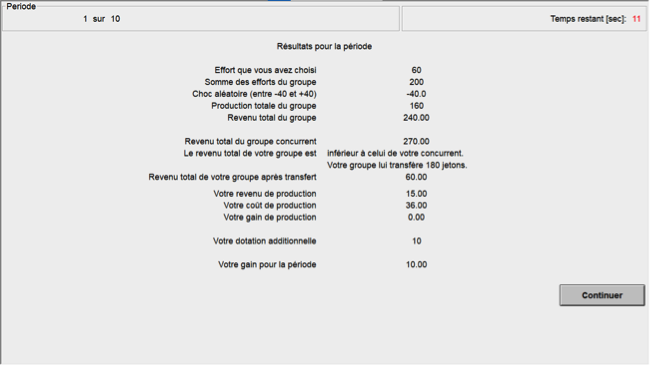
\includegraphics[width = 0.9\textwidth]{05_fig14-annexII.png}

Cliquez sur «Continuer» pour passer à la suite.

\vspace{.3cm}
\ul{Calcul de votre gain pour l'ensemble de l'expérience}

\vspace{.2cm}
Votre gain total en jetons pour l'ensemble de l'expérience égale la
somme de vos gains pour chacune des 10~périodes de l'expérience. À la
fin du jeu apparaît un écran de synthèse vous indiquant pour les
10~périodes votre gain pour chaque période et le cumul des gains de la
période et des périodes précédentes. Le cumul de vos gains à l'issue de
la dixième période correspond à votre gain total en jetons à l'issue de
l'expérience.

\section{Questionnaire post-expérience --\\ pour tous les traitements}
\label{Annexe:Questionnaire}

\subsection{Questions concernant les caractéristiques sociodémographiques des participants}

--~\emph{Quel âge avez-vous~?}

--~\emph{Quel est votre genre~?} Masculin / Féminin

--~\emph{Le français est-il votre langue maternelle~?} Oui / Non

--~\emph{Êtes-vous un(e) étudiant(e) étranger(ère)~?} Oui / Non / Je ne suis
pas étudiant(e)/Je préfère ne pas répondre

--~\emph{Quel est votre niveau d'étude~?} Licence~1 / Licence~2 /
Licence 3 / Master 1 / Master 2 / \textgreater Master / Autres

--~\emph{Quelle est votre discipline actuelle~?} Sciences économiques /
Administration sociale et économique / Droit / Gestion / Sciences
politiques / Littérature / Chimie / Physique / Médecine / Autres

--~\emph{Quelle université ou école fréquentez-vous~?} Université /
École de commerce / École d'ingénieur / Autres

--~\emph{À combien de session(s) expérimentale(s) rémunérée(s) avez-vous
participé avant cette session~?} Jamais / Une / Deux ou plus


\subsection{Questions concernant le jeu (questions ouvertes)}

\emph{--~Les règles du jeu vous ont-elles paru claires~?}

\emph{--~Quelle a été votre stratégie de jeu~?}

\emph{--~À votre avis, quel est le but de cette expérience~?}

\section{Éléments statistiques supplémentaires}
\label{Annexe:Éléments stats}

Les éléments statistiques supplémentaires concernent les points
suivants~:

1.~Significativité des différences de caractéristiques démographiques
entre participants aux différents traitements.

2.~Analyse statistique du comportement de sanction dans le traitement
avec Pression des pairs.

3.~Évolution de la dispersion des efforts au sein des équipes, dans le
traitement avec Objectif d'équipe.

4.~Significativité des différences de profits des firmes et du revenu
total entre traitements.

5.~Évolution de la composition de la richesse totale au fil du temps par
traitement.


\subsection{Significativité des différences de caractéristiques
démographiques entre participants aux différents traitements}
\label{Annexe:Significativité différences}

%Tableau A1

{\centering \textsc{Tableau A1} -- \emph{Résultats des tests sur les différences sociodémographiques\\ entre traitements}\par}

\begin{table}[h!]
% \caption{Résultats des tests sur les différences sociodémographiques\\ entre traitements}
\label{tab_A1}
\centering
\begin{tabular}{p{4.2cm}D{1cm}D{1.2cm}D{1.670cm}D{1cm}}
\toprule
    & Genre* & Participation* & Sciences économiques* & Âge\textsuperscript{≠} \tabularnewline
\midrule
Baseline \emph{vs} Pression pairs & 0,371 & 1,000 & 0,666 & 0,5905 \tabularnewline
Baseline \emph{vs} Objectif d'équipe & 0,770 & 0,048 & 0,416 & 0,8892 \tabularnewline
Baseline \emph{vs} Tournois entre équipes & 0,803 & 0,007 & 0,196 & 0,8978 \tabularnewline
Pression pairs \emph{vs} Objectif d'équipe & 0,760 & 0,137 & 1,000 & 0,4223 \tabularnewline
Pression pairs \emph{vs} Tournois entre équipes & 0,439 & 0,023 & 0,759 & 0,3103 \tabularnewline
Objectif d'équipe \emph{vs} Tournois entre équipes & 0,803 & 0,794 & 1,000 & 0,9416 \tabularnewline
\bottomrule
\end{tabular}
\notedetableau{*~Test exact de Fisher~; χ\textsuperscript{2} tests
donnent des résultats qualitativement similaires.
\textsuperscript{≠}~\emph{t}-test.}
\end{table}


\subsection{Analyse statistique du comportement de sanction\\ dans le
traitement avec Pression des pairs}
\label{Annexe:Analyse statist comport}

\vspace{.2cm}
Dans un premier temps, nous présentons les statistiques sur l'évolution
de la proportion de punisseurs au fil du temps. Ensuite, nous présentons
une analyse comparée des caractéristiques et du comportement des
punisseurs ultimes (c'est-à-dire ceux qui punissent lors de la dernière
période du jeu) et de ceux qui ne sont pas punisseurs ultimes.

\begin{figure}[h]
    \centering
    \caption{Évolution de la proportion de punisseurs au fil du temps}
    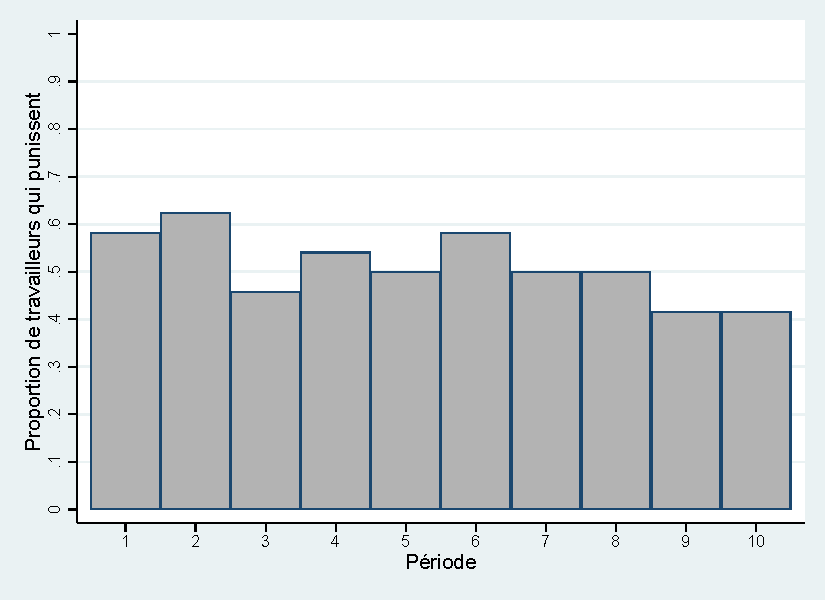
\includegraphics[height=6cm]{05_graphA1.pdf}
\end{figure}

La figure~A1 présente l'évolution de la proportion de punisseurs au
cours du temps. Il indique que cette proportion est plutôt stable. La
différence de proportion de punisseurs entre les cinq premières périodes
et les cinq dernières n'est pas significative selon un test de Fisher
non paramétrique (\emph{p}~=~0,439).

Parmi les 24~participants ayant joué le traitement Pression des pairs,
10 punissent lors de la période~10. Nous les appelons punisseurs
ultimes. Il est intéressant de mieux comprendre ces punisseurs ultimes
puisqu'ils ne punissent pas pour des raisons stratégiques, c'est-à-dire
en vue de favoriser une coopération future. Une explication possible est
que ces punisseurs ultimes sont motivés par des raisons non
stratégiques, telles que la réciprocité, la vengeance aveugle
(\textcite{Nikiforakis2004}~; \textcite{DenantBoemontMascletNoussair2007}), voire une pure volonté de nuire aux autres (\emph{pure
nastiness}) ou un désir de domination (\textcite{Zizzo2003}~; \textcite{CinyabugumaPagePutterman2004}, \textcite{CinyabugumaPagePutterman2006}). D'autres travaux antérieurs ont étudié la relation entre les émotions et la volonté de punir, et en
particulier comment la colère accompagne l'application d'une punition
coûteuse dans les interactions bilatérales (\textcite{BosmanVanWinden2002}~; \textcite{BenShakharBornsteinHopfensitzVanWinden2007}) ou dans des jeux de bien
public avec sanction (voir par exemple \textcite{JoffilyMascletNoussairVilleval2014}~; \textcite{DickinsonMasclet2015}). Ces études mesurent les
émotions au moyen d'auto-évaluations ou en utilisant des mesures
électrophysiologiques de l'excitation émotionnelle.

Les tableaux~A2 et A3 présentent des statistiques descriptives
concernant les efforts, les points attribués et les données
démographiques pour les 10~punisseurs ultimes et les autres punisseurs,
respectivement.

\vspace{0.2cm}
{\centering \textsc{Tableau A2} -- \emph{Statistiques descriptives concernant les punisseurs ultimes}\par}
\begin{table}[h!]
% \caption{Statistiques descriptives concernant les punisseurs ultimes}
\label{tab_A2}
\centering
\begin{tabular}{p{2.8cm}D{1.2cm}D{1.2cm}D{1.2cm}D{1cm}D{1cm}}
\toprule
& Observations & Moyenne & Écart type & Min & Max \tabularnewline
\midrule
Effort & 100 & 58,13 & 20,69 & 10 & 100 \tabularnewline
Points attribués & 100 & 2,1 & 2,35 & 0 & 9 \tabularnewline
Genre & 10 & 0,1 & 0,32 & 0 & 1 \tabularnewline
Participation précédente & 10 & 0 & 0 & 0 & 0 \tabularnewline
Sciences économiques & 10 & 0,1 & 0,32 & 0 & 1 \tabularnewline
Âge & 10 & 21,1 & 1,73 & 18 & 24 \tabularnewline
\bottomrule
\end{tabular}
\end{table}

\vspace{0.2cm}
{\centering \textsc{Tableau A3} -- \emph{Statistiques descriptives concernant les non-punisseurs ultimes}\par}
\begin{table}[h!]
% \caption{Statistiques descriptives concernant les non-punisseurs ultimes}
\label{tab_A3}
\centering
\begin{tabular}{p{2.8cm}D{1.2cm}D{1.2cm}D{1.2cm}D{1cm}D{1cm}}
\toprule
& Observations & Moyenne & Écart type & Min & Max \tabularnewline
\midrule
Effort & 140 & 53,96 & 26,02 & 0 & 100 \tabularnewline
Points attribués & 140 & 1,62 & 2,47 & 0 & 10 \tabularnewline
Genre & 14 & 0,43 & 0,51 & 0 & 1 \tabularnewline
Participation précédente & 14 & 0,14 & 0,36 & 0 & 1 \tabularnewline
Sciences économiques & 14 & 0,21 & 0,43 & 0 & 1 \tabularnewline
Âge & 14 & 20,86 & 2,68 & 18 & 27 \tabularnewline
\bottomrule
\end{tabular}
\end{table}

Le tableau~A4 présente les résultats de tests statistiques afin de
vérifier s'il existe ou pas des différences d'effort, de points
attribués et de caractéristiques démographiques entre les punisseurs
ultimes et les autres. Ce tableau indique l'absence de différences
significatives entre ces différents punisseurs. Autrement dit, il semble
que les punisseurs ultimes ne sont pas significativement différents des
autres punisseurs.

\vspace{0.2cm}
{\centering \textsc{Tableau A4} -- \emph{Significativité des différences entre punisseurs ultimes et les autres}\par}
\begin{table}[h!]
% \caption{Significativité des différences entre punisseurs ultimes et
% les autres}
\label{tab_A4}
\centering
\begin{tabular}{m{2.2cm}D{0.5cm}D{1.1cm}D{0.75cm}D{1.4cm}D{1.6cm}D{0.6cm}}
\toprule
& Effort & Points attribués\textsuperscript{≠} & Genre* & Participation précédente* & Sciences économiques* & Âge\textsuperscript{≠} \tabularnewline
\midrule
Punisseurs ultimes \emph{vs} Autres & 0,18 & 0,13 & 0,17 & 0,49 & 0,44 & 0,80 \tabularnewline
\bottomrule
\end{tabular}
\notedetableau{*~Test exact de Fisher~; \textsuperscript{≠}~\emph{t}-test.}
\end{table}

\begin{figure}[h]
    \centering
    \caption{Évolution du nombre moyen de points attribués par les punisseurs ultimes}
    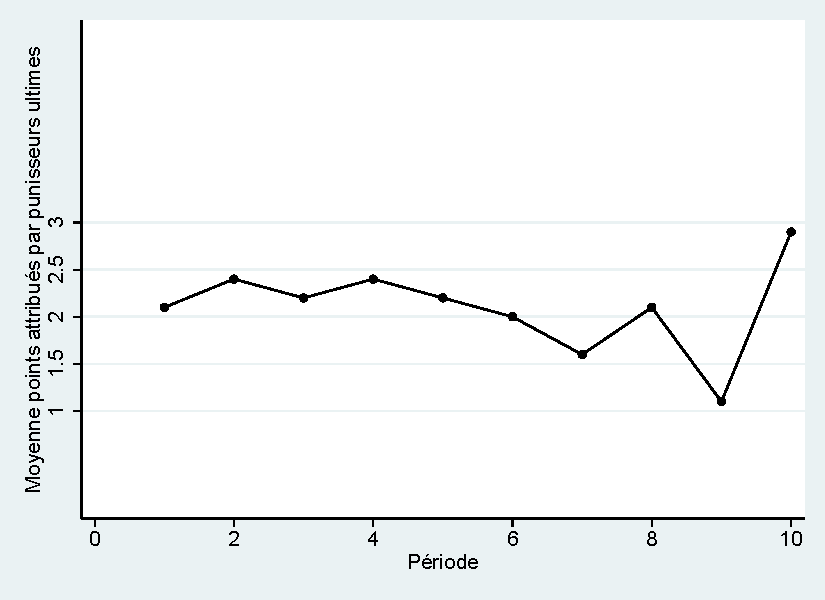
\includegraphics[height=6cm]{05_graphA2.pdf}
\end{figure}

La figure~A2 montre l'évolution du nombre moyen de points de sanction
attribués par les punisseurs ultimes. On note d'abord une légère baisse
du niveau moyen de punition, puis une forte hausse lors de la période
finale, qui pourrait être interprétée comme un effet de fin de partie.
Les punisseurs ultimes attribuent en moyenne 2,9~points lors de la
période~10.

\begin{figure}[h]
    \centering
    \caption{Évolution du nombre moyen de points attribués par les non-punisseurs ultimes}
    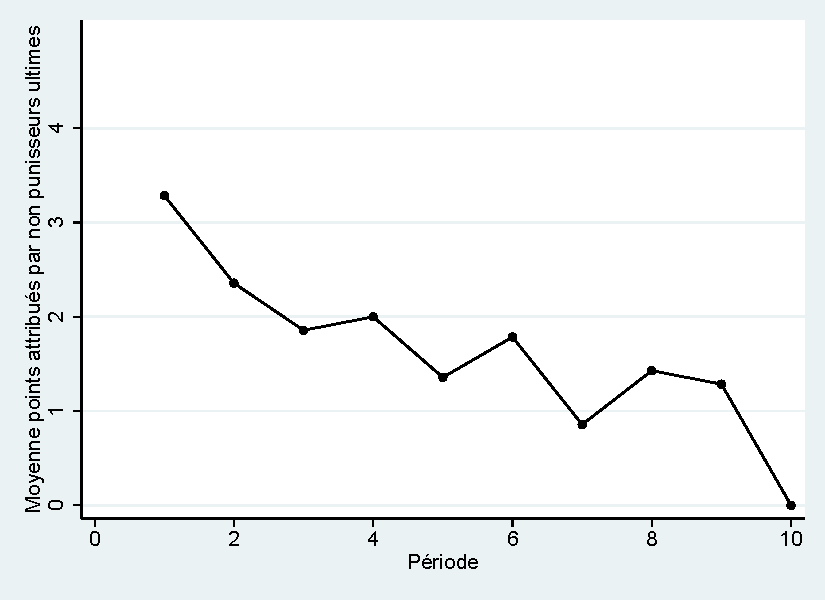
\includegraphics[height=6cm]{05_graphA3.pdf}
\end{figure}

La figure~A3 présente l'évolution du nombre moyen de points attribués
par ceux qui ne sont pas punisseurs ultimes. Elle fait apparaître une
tendance négative.

\newpage

\subsection{Évolution de la dispersion des efforts au sein des équipes, dans
le traitement avec Objectif d'équipe}
\label{Annexe:Évolution dispersion des efforts}

L'analyse de la dispersion de l'effort et de son évolution dans le temps
est présentée graphiquement, à l'aide de boîtes à moustaches. Cette
analyse est réalisée séparément pour les équipes qui parviennent à
atteindre l'objectif et pour les équipes qui ne parviennent pas à
atteindre cet objectif. À noter que les équipes qui réussissent ou
échouent à atteindre l'objectif peuvent changer d'une période à l'autre.

La figure~A4 montre l'évolution de la dispersion des efforts des
travailleurs des équipes qui atteignent l'objectif fixé par
l'entreprise.

\begin{figure}[h!]
    \centering
    \caption{Évolution de la dispersion des efforts, dans l'ensemble des équipes qui atteignent l'objectif}
    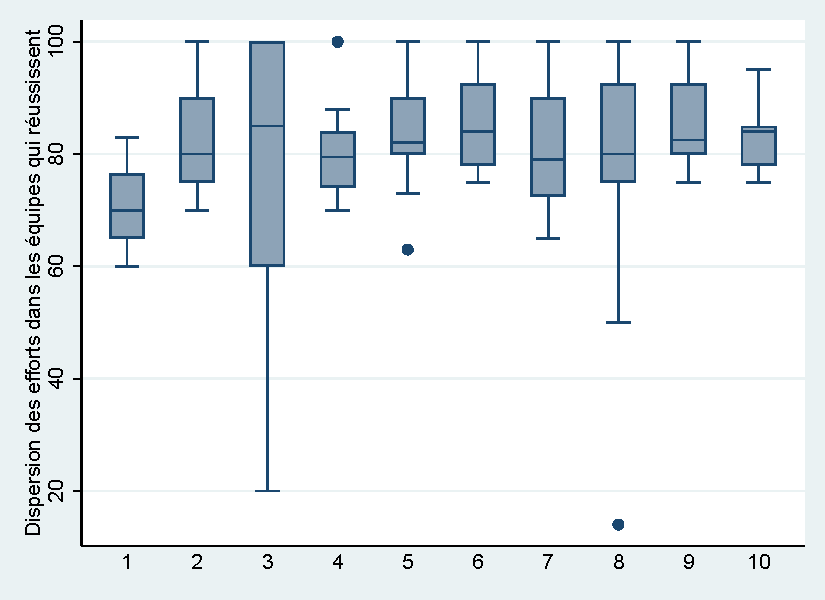
\includegraphics[height=6cm]{05_graphA4.pdf}
\notedetableau{Les boîtes à moustaches indiquent les quartiles. La ligne
au milieu de chaque case correspond à la médiane. La limite inférieure
de chaque case correspond au premier quartile et la limite supérieure au
troisième quartile. La moustache inférieure est égale au maximum entre
le minimum de la distribution et le premier quartile moins 1,5~fois la
différence entre le troisième et le premier quartile. La moustache la
plus élevée est égale au minimum entre le maximum de la distribution et
le troisième quartile plus 1,5~fois la différence entre le troisième et
le premier quartile. Les points correspondent aux valeurs extrêmes, soit
sous la moustache inférieure, soit au-dessus de la moustache supérieure.
Ils correspondent aux valeurs aberrantes, c'est-à-dire des points de
données qui se situent à une distance significative des autres valeurs
de l'échantillon.}
\end{figure}

La figure~A4 ne montre aucune tendance claire de réduction de la
dispersion des efforts parmi les travailleurs des équipes qui atteignent
l'objectif.
La figure~A5 présente plus en détail l'évolution de la dispersion des
efforts entre les travailleurs au sein de chaque équipe lorsque celle-ci
atteint l'objectif.

\begin{figure}[h]
    \centering
    \caption{Évolution de la dispersion des efforts, au sein de chacune des équipes lorsqu'elles atteignent l'objectif}
    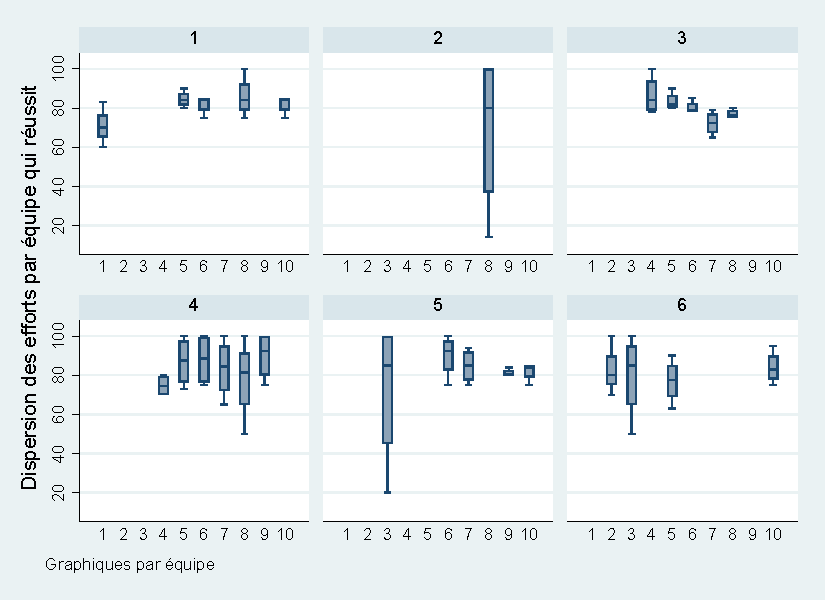
\includegraphics[height=6cm]{05_graphA5.pdf}
\end{figure}

La figure~A5 ne présente pas non plus de tendance claire à la
réduction de la dispersion des efforts des travailleurs, au sein des
équipes qui atteignent l'objectif.
La figure~A6 montre l'évolution de la dispersion des efforts entre
les travailleurs de toutes les équipes qui n'atteignent pas l'objectif.
Elle indique que le niveau de dispersion des efforts est relativement
élevé dans les équipes qui échouent à atteindre l'objectif contrairement
aux équipes qui réussissent (figure~A4). À noter que les équipes qui
échouent peuvent manquer d'atteindre l'objectif malgré des efforts
relativement élevés de leurs membres, en raison d'un choc de production
aléatoire négatif. La figure ne montre pas de réduction de la
dispersion des efforts ni d'indice de découragement des travailleurs.

\begin{figure}[h]
    \centering
    \caption{Évolution de la dispersion des efforts, dans l'ensemble des équipes qui n'atteignent pas l'objectif}
    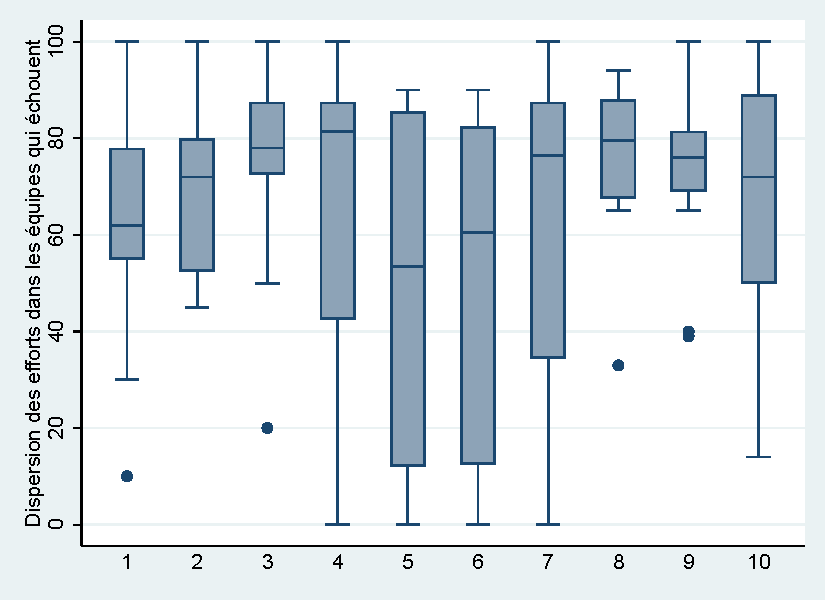
\includegraphics[height=6cm]{05_graphA6.pdf}
\notedetableau{Les boîtes à moustaches indiquent les quartiles. La ligne
au milieu de chaque case correspond à la médiane. La limite inférieure
de chaque case correspond au premier quartile et la limite supérieure au
troisième quartile. La moustache inférieure est égale au maximum entre
le minimum de la distribution et le premier quartile moins 1,5~fois la
différence entre le troisième et le premier quartile. La moustache la
plus élevée est égale au minimum entre le maximum de la distribution et
le troisième quartile plus 1,5~fois la différence entre le troisième et
le premier quartile. Les points correspondent aux valeurs extrêmes, soit
sous la moustache inférieure, soit au-dessus de la moustache supérieure.
Ils correspondent aux valeurs aberrantes, c'est-à-dire des points de
données qui se situent à une distance significative des autres valeurs
de l'échantillon.}
\end{figure}

La figure~A7 analyse plus en détail l'évolution de la dispersion des
efforts entre les travailleurs au sein de chaque équipe dès lors
qu'elles n'atteignent pas l'objectif. Elle indique également davantage de
dispersion que dans le cas des équipes qui atteignent l'objectif
(figure~A5). Cette figure ne montre aucune tendance à la réduction de
la dispersion des efforts dans les équipes qui échouent à atteindre
l'objectif.

\begin{figure}[h]
    \centering
    \caption{Évolution de la dispersion des efforts, au sein de chacune des équipes lorsqu'elles n'atteignent pas l'objectif}
    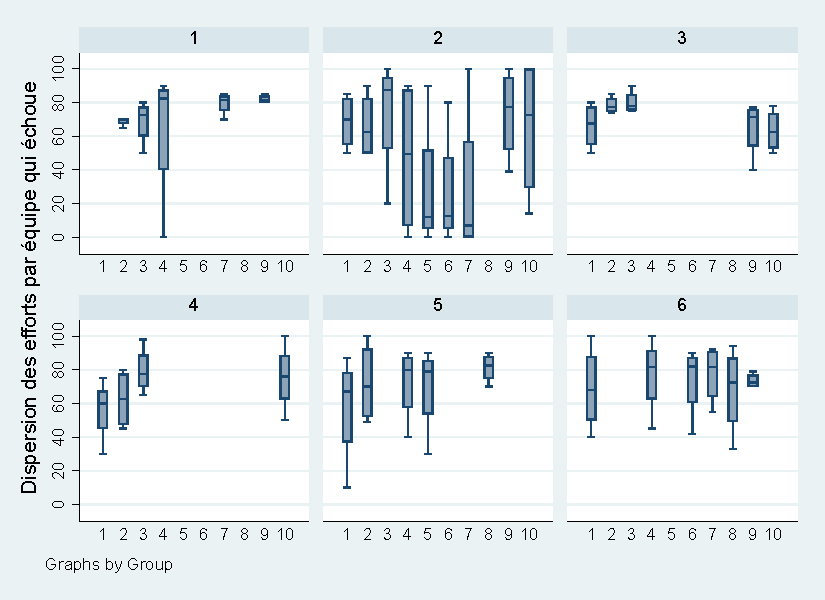
\includegraphics[height=6cm]{05_graphA7.pdf}
\end{figure}

\subsection{Significativité des différences de profits des firmes\\ et du revenu total entre traitements}
\label{Annexe:Significativité différences de profits}

\vspace{0.2cm}
{\centering \textsc{Tableau A5} -- \emph{Significativité des différences de coefficients de régression entre traitements}\par}
\begin{table}[h!]
% \caption{Significativité des différences de coefficients de régression entre traitements}
\label{tab_A5}
\centering
\begin{tabular}{m{2.6cm}D{2.3cm}D{2.3cm}D{2.3cm}}
\toprule
& Pression pairs \emph{vs} Objectif équipe & Pression pairs \emph{vs} Tournois équipes & Objectif équipe \emph{vs} Tournois équipes \tabularnewline
\midrule
Profit des firmes & 0,0000 & 0,2423 & 0,0000 \tabularnewline
Richesse totale & 0,0004 & 0,0075 & 0,1669 \tabularnewline
\bottomrule
\end{tabular}
\notedetableau{Test d'égalité des coefficients de régression.}
\end{table}

\subsection{Évolution de la répartition de la richesse totale\\ entre
l'entreprise et les travailleurs au fil du temps par traitement}
\label{Annexe:Évolution répartition}

\begin{figure}[h]
    \centering
    \caption{Évolution de la répartition de la richesse totale dans le
traitement Baseline}
    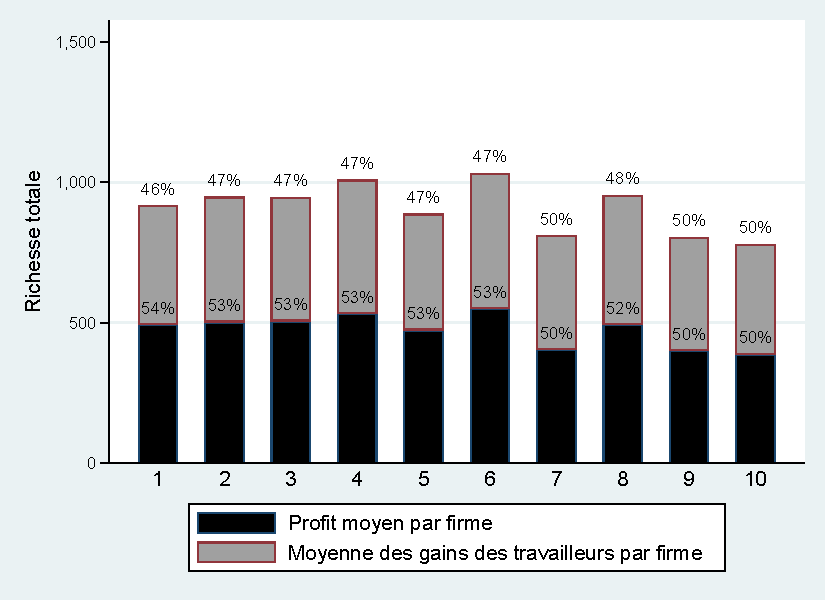
\includegraphics[height=6cm]{05_graphA8.pdf}
\end{figure}

\vspace{0.2cm}
La figure~A8 indique l'évolution de la répartition de la richesse
totale entre l'entreprise et les travailleurs au cours du temps dans le
traitement Baseline. Le partage de la richesse produite est relativement
égalitaire autour de 50~\% et ce ratio demeure stable au cours du temps.

\begin{figure}[h]
    \centering
    \caption{Évolution de la répartition de la richesse totale dans le traitement Pression des pairs}
    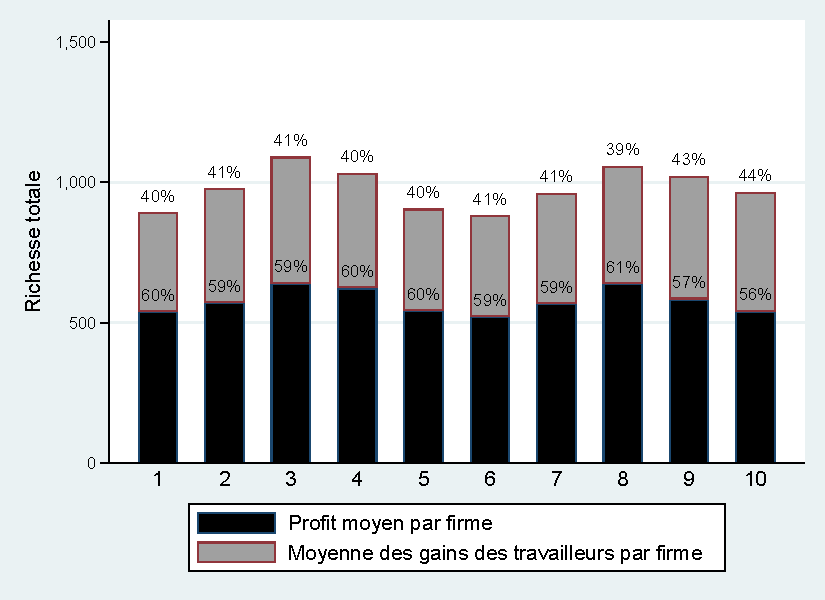
\includegraphics[height=6cm]{05_graphA9.pdf}
\end{figure}

La figure~A9 indique l'évolution de la répartition de la richesse
totale entre l'entreprise et les travailleurs au cours du temps dans le
traitement Pression des pairs. Le partage de la richesse produite est
légèrement en faveur de l'entreprise et ce ratio varie entre 56 et
61~\%. Ce ratio demeure assez stable au cours du temps.

\begin{figure}[h]
    \centering
    \caption{Évolution de la répartition de la richesse totale dans le traitement Objectif d'équipe}
    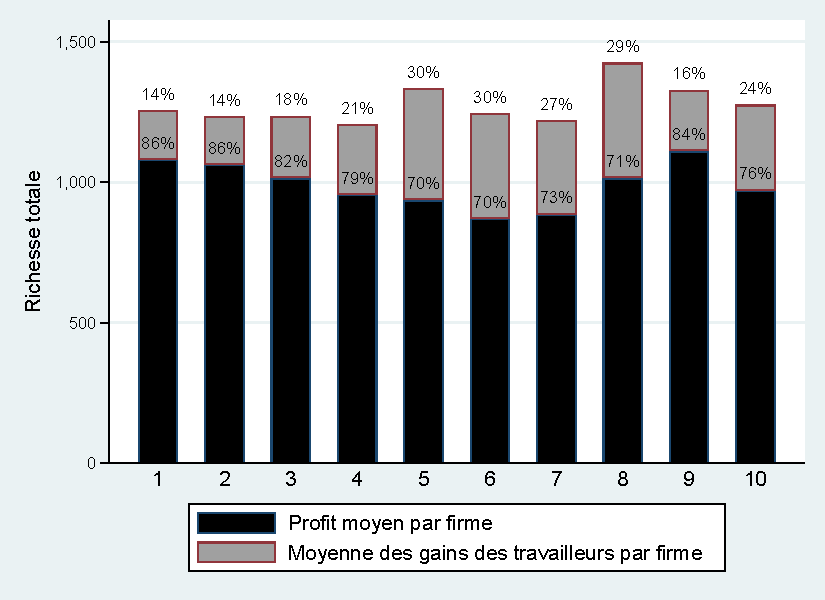
\includegraphics[height=6cm]{05_graphA10.pdf}
\end{figure}

La figure~A10 indique l'évolution de la répartition de la richesse
totale entre l'entreprise et les travailleurs au cours du temps dans le
traitement Objectif d'équipe. Le partage de la richesse produite est
très inégalitaire puisqu'elle est très largement en faveur de
l'entreprise et ce ratio varie entre 70 et 86~\%. On observe une légère
diminution de ce ratio au cours du temps.

\begin{figure}[h]
    \centering
    \caption{Évolution de la répartition de la richesse totale dans le traitement Tournois entre équipes}
    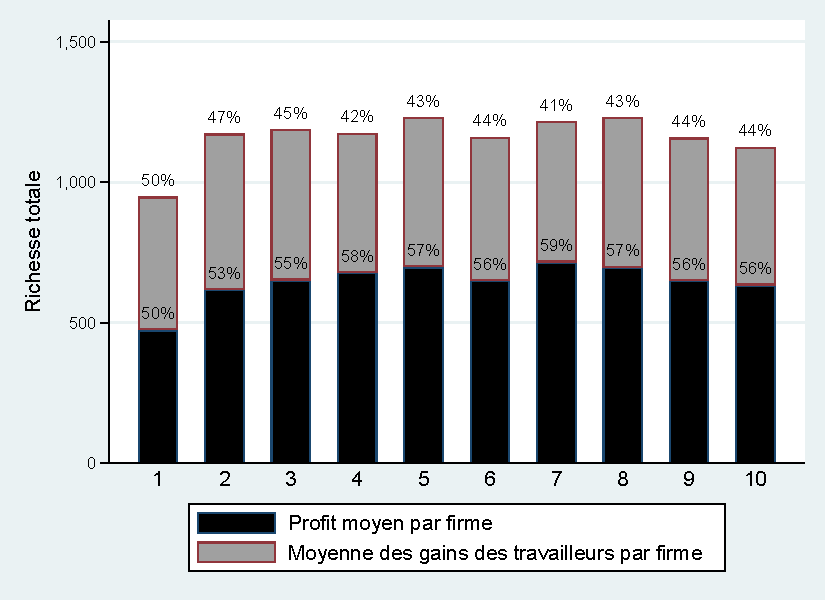
\includegraphics[height=6cm]{05_graphA11.pdf}
\end{figure}

La figure~A11 indique l'évolution de la répartition de la richesse
totale entre l'entreprise et les travailleurs au cours du temps dans le
traitement Tournois entre équipes. Le partage de la richesse produite
est assez égalitaire même s'il est légèrement en faveur de l'entreprise.
Ce ratio varie entre 50 et 59~\% et demeure assez stable au cours du
temps.

\end{appendices}

\end{refsection}

\end{Article}
